\documentclass[letterpaper,final,12pt,reqno]{amsart}

\usepackage[total={6.3in,9.2in},top=1.1in,left=1.1in]{geometry}

\usepackage{verbatim}
\usepackage{empheq}
\usepackage[dvipsnames]{xcolor}
\usepackage{animate}
\usepackage{graphicx}
\usepackage{fancyvrb}

%\usepackage{palatino}

% hyperref should be the last package we load
\usepackage[pdftex,
colorlinks=true,
plainpages=false, % only if colorlinks=true
linkcolor=blue,   % only if colorlinks=true
citecolor=Red,   % only if colorlinks=true
urlcolor=ForestGreen     % only if colorlinks=true
]{hyperref}

\pdfinfo{
/Title (Numerical modelling of glaciers, ice sheets, and ice shelves)
/Author (Ed Bueler)
/Subject (numerical modelling of ice sheets)
/Keywords (numerical modelling, numerical analysis, glacier, ice sheet, ice shelf, shallow models)
}

\renewcommand{\baselinestretch}{1.05}

\newcommand{\ddt}[1]{\ensuremath{\frac{\partial #1}{\partial t}}}
\newcommand{\ddx}[1]{\ensuremath{\frac{\partial #1}{\partial x}}}
\newcommand{\ddy}[1]{\ensuremath{\frac{\partial #1}{\partial y}}}
\newcommand{\pp}[2]{\ensuremath{\frac{\partial #1}{\partial #2}}}
\renewcommand{\t}[1]{\texttt{#1}}
\newcommand{\Matlab}{\textsc{Matlab}\xspace}
\newcommand{\bq}{\mathbf{q}}
\newcommand{\bu}{\mathbf{u}}
\newcommand{\bU}{\mathbf{U}}
\newcommand{\eps}{\epsilon}
\newcommand{\grad}{\nabla}
\newcommand{\Div}{\nabla\cdot}
\newcommand{\devstress}{\tau}

\newcommand{\minput}[1]{
\vspace{0.8cm}
\VerbatimInput[frame=single,framesep=3mm,label=\fbox{\normalsize \textsl{\,#1.m\,}},fontfamily=courier,fontsize=\footnotesize]{tmp/#1.slim.m}
\vspace{0.5cm}
}

% usage:  \onefigsize{name}{caption}{width}
\newcommand{\onefigsize}[3]{
\begin{figure}[ht]
\centering
\includegraphics[width=#3,keepaspectratio=true]{#1}
\caption{#2}
\label{fig:#1}
\end{figure}}

% usage:  \onefig{name}{caption}
\newcommand{\onefig}[2]{\onefigsize{#1}{#2}{3.0in}}

% usage:  \twofigsizes{left-name}{right-name}{caption}{left-width}{right-width}
\newcommand{\twofigsizes}[5]{
\begin{figure}[ht]
\centering
\includegraphics[width=#4,keepaspectratio=true]{#1} \quad
\includegraphics[width=#5,keepaspectratio=true]{#2}
\caption{#3}
\label{fig:#1}
\end{figure}}

% usage:  \twofig{left-name}{right-name}{caption}
\newcommand{\twofig}[3]{\twofigsizes{#1}{#2}{#3}{2.5in}{2.5in}}



\begin{document}
\graphicspath{{../figures/}}

\begin{titlepage}

  \begin{center}
  \phantom{foo}
    \vspace{1.0cm}

     {\Large \textsc{Numerical modelling}}
    \vspace{0.7cm}

     {\Large \textsc{of glaciers, ice sheets, and ice shelves}}

    \vspace{1.5cm}

    {\large Ed Bueler}
    \vspace{1cm}

    International Summer School in Glaciology

    McCarthy Alaska, June 2016

    \vfill
    
    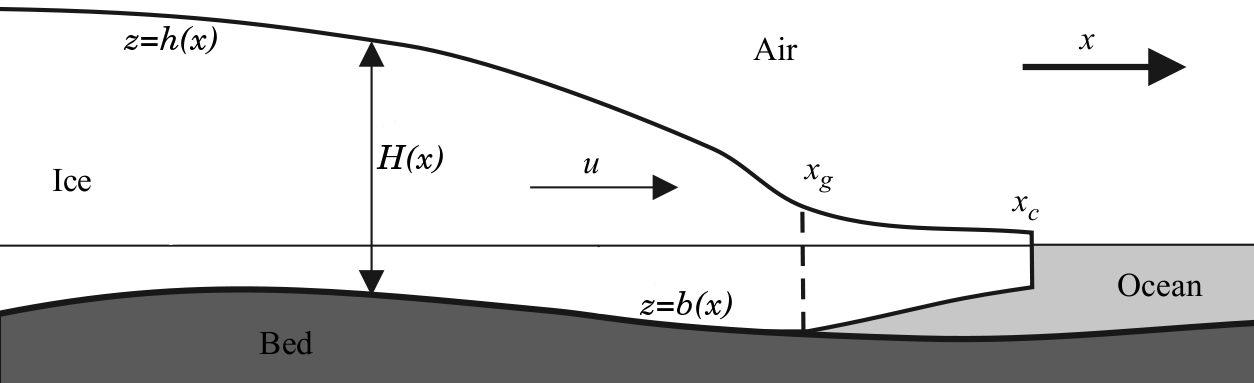
\includegraphics[width=6.0in]{flowline}
  
    \scriptsize \emph{Illustrates the notation used in these notes.  Figure modified from \cite{SchoofMarine1}.} \normalsize
    
    \vspace{1.5in}
  \end{center}
\end{titlepage}

\clearpage\newpage

%\setcounter{section}{1}
\section{Introduction}

The greatest importance of numerical models in glaciology is introspective.  You should ask yourself: When I combine my imperfect and incomplete understanding of glacier processes into this mathematical model which I put on a computer, does it behave as I expect?  Numerical models can indeed show how processes interact to give overall behavior.  They can at least demonstrate flaws in our understanding of those processes.  But they should be built with care.  An avoidable bad outcome is to spend time---or worse, reputation---interpreting, explaining, or justifying numerical model behavior that is in fact an artifact of poor computer programming or numerical analysis.

So the reader of these notes may be surprised that a continuum model, and not a computer code, seems to be our focus much of the time.  While all codes produce some numbers, we want numbers that actually come from the continuum model we have written down.  We will therefore analyse numerical implementations to see if they match the model equations and their solutions.

These notes have a limited scope:
  \begin{quote}\emph{shallow approximations of ice flow.}\end{quote}
They adopt a constructive approach; we provide:
  \begin{quote}\emph{example numerical codes that actually work.}\end{quote}
Within our scope are the shallow ice approximation (SIA) in two horizontal dimensions (2D), the shallow shelf approximation (SSA) in 1D, and the mass continuity and surface kinematical equations.  We recall the Stokes model, but we do not address its numerical solution.  Our numerical concepts include finite difference schemes, solving algebraic systems from stress balances, and the verification of codes using exact solutions.

Our notation, which generally follows \cite{GreveBlatter2009}, is common in the glaciological literature, but see Table \ref{tab:notation}.  Cartesian coordinates are $x,y,z$ with $z$ positive-upward.  If these coordinates or time $t$ appear as subscripts then they denote partial derivatives: $u_x = \partial u/\partial x$.  Tensor notation uses subscripts from the list $\{1,2,3,i,j\}$.  For example, ``$\tau_{ij}$'' or ``$\tau_{13}$'' denote entries of the deviatoric stress tensor.

These notes are based on nineteen Matlab codes, each about one-half page.  All have been tested in Matlab and Octave.  They are distributed by cloning the repository at
\begin{quote}
\url{https://github.com/bueler/mccarthy}
\end{quote}
\noindent and looking in the \texttt{mfiles/} subdirectory.  Five of these codes are printed here, with their comments stripped for compactness and clarity.  The electronic versions have generous comments and help files.

\begin{table}[ht]
\caption{Notation used in these notes, with values for some constants.}
\begin{tabular}{clll}
variable  & description & SI units & value \\
\hline
$A$ & $A=A(T)=$ ice softness in the Glen flow law & $\text{Pa}^{-n}\,\text{s}^{-1}$ \\
$B$ & ice hardness; $B=A^{-1/n}$ & $\text{Pa}\,\text{s}^{1/n}$ \\
$b$ & bedrock elevation & m \\
$c$ & specific heat in general & J kg$^{-1}$ K$^{-1}$ \\
$\nabla$ & (spatial) gradient & m$^{-1}$ \\
$\nabla\cdot$ & (spatial) divergence & m$^{-1}$ \\
$\mathbf{g}$ & gravity & m s$^{-2}$\phantom{foobar} & 9.81 \\
$H$ & ice thickness & m \\
$h$ & ice surface elevation & m \\
$\kappa$ & conductivity in general & J s$^{-1}$ m$^{-1}$ K$^{-1}$ \\
$M$ & climatic mass balance & m s$^{-1}$ \\
$n$ & exponent in Glen flow law & & 3 \\
$\nu$ & viscosity & Pa s \\
$p$ & pressure & Pa \\
$\bq$ & map-plane ice flux: $\bq = \int_{b}^{h} \bU\,dx = \bar{\bU} H$ & $\text{m}^2\,\text{s}^{-1}$ \\
$\rho$ & density of ice & kg m$^{-3}$ & 910 \\
$\rho_w$ & density of sea water & kg m$^{-3}$ & 1028 \\
$T$ & temperature & K \\
$\tau$ & norm (second invariant) of $\tau_{ij}$: $2 \tau^2 = \sum_{ij} \tau_{ij}^2$ & Pa \\
$\tau_{ij}$ & deviatoric stress tensor & Pa \\
$Du_{ij}$ & strain rate tensor & s$^{-1}$ \\
$\mathbf{U}$ & $=(u,v)$ horizontal ice velocity & m s$^{-1}$ \\
$\mathbf{u}$ & $=(u,v,w)$ 3D ice velocity & m s$^{-1}$ \\
\end{tabular}
\label{tab:notation}
\end{table}


\section{Ice flow equations}

My first goal in these notes is to get to an equation for which I can say:
\begin{center}
\emph{by numerically solving this equation, we have a usable model for an ice sheet.}
\end{center}
\noindent A ``usable'' model tends to be \emph{understood} as much as it is \emph{correct}.  Also, this first usable model will not be complete by any modern standard.  To get to my goal I first (briefly!) recall the continuum mechanical equations of ice flow.

Ice in glaciers is a moving fluid so we describe its motion by a velocity field $\mathbf{u}(t,x,y,z)$.  If the ice fluid were faster-moving than it actually is, and if it were linearly-viscous like liquid water, then it would be a ``typical'' incompressible fluid.  We would use the Navier-Stokes equations as the model:
\begin{align}
\nabla \cdot \mathbf{u} &= 0 &&\text{\emph{incompressibility}} \label{incompressible} \\
\rho \left(\mathbf{u}_t + \mathbf{u}\cdot\nabla \mathbf{u}\right) &= -\nabla p + \nabla \cdot (\nu \nabla \mathbf{u}) + \rho \mathbf{g} &&\text{\emph{stress balance}} \label{navierstokes}
\end{align}
In equation \eqref{navierstokes} the term $\mathbf{u}_t + \mathbf{u}\cdot\nabla \mathbf{u}$ is an acceleration.  The right-hand side of \eqref{navierstokes} is the total stress, and so equation \eqref{navierstokes} says ``$ma=F$'', i.e.~it is Newton's second law.  Much time has been spent to get partial understanding of the rich solutions of these Navier-Stokes equations; a book-length introduction like \cite{Acheson} is recommended.  The numerical solution of these equations is \emph{computational fluid dynamics} (CFD).

But, is ice flow modelling a part of CFD?  (And does a well-written general-purpose CFD text like \cite{Wesseling} help the glaciers student?)  It is true that ice sheet flow can be a large-scale fluid problem like atmosphere and ocean circulation in climate systems, but it is an odd one.  Consider some topics which might make ocean circulation modelling exciting, for example:
  \begin{center} turbulence \qquad convection \qquad  coriolis force  \qquad density stratification
  \end{center}
None of these topics are relevant to ice flow.  What could be interesting about the flow of slow, and surely boring, ice?

First observe that ice is indeed a slow fluid.  In terms of equation \eqref{navierstokes}, ``slow'' means $\rho \left(\mathbf{u}_t + \mathbf{u}\cdot\nabla \mathbf{u}\right) \approx 0$, which says that the forces (stresses) of inertia are negligible.  However, ice is also a shear-thinning fluid with a specific kind of nonlinearly-viscous (``non-Newtonian'') behavior in which larger shear strain rates imply smaller viscosity.  The viscosity $\nu$ in \eqref{navierstokes} is therefore not constant, and so we must separately state an empirically-based flow law in addition to restating \eqref{navierstokes} for slow flows.

\subsection*{Stokes equations}  The standard model for isothermal ice flow is this set of equations:
\begin{align}
\nabla \cdot \mathbf{u} &= 0 &&\text{\emph{incompressibility}} \label{incompressibleagain} \\
0 &= - \nabla p + \nabla \cdot \tau_{ij} + \rho \mathbf{g} &&\text{\emph{stress balance}} \label{forcebalance} \\
Du_{ij} &= A \tau^2 \tau_{ij} &&\text{\emph{$n$=3 Glen flow law}} \label{flowlaw}
\end{align}
In the flow law \eqref{flowlaw}, the deviatoric stress tensor $\tau_{ij}$ and the strain rate tensor $Du_{ij}$ appear; previous lectures cover these.  Here we merely note that: $Du_{ij} = (1/2)((u_i)_{x_j}+(u_j)_{x_i})$ if we index coordinates by $x_1,x_2,x_3=x,y,z$, each tensor in \eqref{flowlaw} is symmetric and has trace zero, and $\tau^2 = (1/2) \tau_{ij} \tau_{ij}$ (using the summation convention).

The Stokes equations do not contain a time derivative.  Thus boundary stresses, the force of gravity $\rho \mathbf{g}$, and ice softness $A$ together determine the velocity and stress fields (i.e.~$\bu$, $p$, $\tau_{ij}$) instantaneously.  Thus ice flow simulation codes have no memory of prior momentum or velocity.  Said another way, velocity is a ``diagnostic'' output of ice flow codes, because it is not needed for (re)starting a simulation.

\subsection*{Plane-flow Stokes equations}  Consider now the $x,z$-plane case of equations \eqref{incompressibleagain}, \eqref{forcebalance}, and \eqref{flowlaw}.  ``Plane-flow'' means that velocity component $v$ is zero and that all derivatives with respect to $y$ are zero:
\begin{align}
u_x + w_z &= 0 &&\text{\emph{incompressibility}} \label{incompressiblexz} \\
p_x &= \tau_{11,x} + \tau_{13,z} &&\text{\emph{stress balance} ($x$)} \label{stokespx} \\
p_z &= \tau_{13,x} - \tau_{11,z} - \rho g &&\text{\emph{stress balance} ($z$)} \label{stokespz} \\
u_x &= A \tau^2 \tau_{11} &&\text{\emph{flow law} (diagonal)}  \label{forceflowx} \\
u_z + w _x &= 2 A \tau^2 \tau_{13} &&\text{\emph{flow law} (off-diagonal)} \label{forceflowz}
\end{align}
Note that $\tau_{13}$ is a shear stress while $\tau_{11}$ and $\tau_{33}=-\tau_{11}$ are deviatoric longitudinal stresses.  Also $\tau^2 = \tau_{11}^2+\tau_{13}^2$ in this case.  Equations \eqref{incompressiblexz}--\eqref{forceflowz} form a system of five nonlinear equations in five scalar unknowns ($u,w,p,\tau_{11},\tau_{13}$).

\subsection*{Slab-on-a-slope}  Equations \eqref{incompressiblexz}--\eqref{forceflowz} are complicated enough to make us pause before jumping in to numerical solution methods, but  we can handle a simplified situation first.  A uniform slab of ice, or a ``slab-on-a-slope'', is both a case in which we can actually solve the Stokes equations, and a motivation for the shallow model in the next subsection.

\onefig{slab}{Rotated axes for a slab-on-a-slope flow calculation.}

We rotate our coordinates only for this example and not elsewhere in these notes.  The two-dimensional axes ($x$,$z$) shown in Figure \ref{fig:slab} are rotated downward (clockwise) at angle $\alpha>0$ so that the gravity vector has components $\mathbf{g} = (g \sin\alpha,- g \cos \alpha)$.  Equations \eqref{stokespx} and \eqref{stokespz} in these rotated coordinates are
\begin{align}
p_x &= \tau_{11,x} + \tau_{13,z} + \rho g \sin\alpha, \label{stokespxrot} \\
p_z &= \tau_{13,x} - \tau_{11,z} - \rho g \cos\alpha. \label{stokespzrot}
\end{align}
Assuming also that there is no variation with $x$, the whole set of Stokes equations \eqref{incompressiblexz}, \eqref{forceflowx}, \eqref{forceflowz}, \eqref{stokespxrot}, \eqref{stokespzrot} simplifies greatly:
\begin{align}
w_z &= 0 &   0 &= \tau_{11} \label{stokesslab} \\
\tau_{13,z} &= - \rho g \sin\alpha &   u_z &= 2 A \tau^2 \tau_{13} \notag \\
p_z &= -\tau_{11,z} = - \rho g \cos\alpha \notag
\end{align}
We apply boundary conditions for these functions of $z$: $w(0)=0$, $p(H)=0$, $u(0)=u_0$.  The basal velocity $u_0$ will remain undetermined for now.

By integrating equations \eqref{stokesslab} with respect to $z$, and using $\tau_{11}=0$, we get $w=0$, $p = \rho g \cos\alpha (H-z)$, and $\tau_{13} = \rho g \sin\alpha (H-z)$.  Note that $H-z$ is the depth below the ice surface, so both the pressure $p$ and shear stress $\tau_{13}$ are proportional to depth.  Because $u_z = 2 A \tau^2 \tau_{13}$, by integrating vertically again we find the horizontal velocity:
\begin{align}
u &= u_0 + \frac{1}{2} A (\rho g \sin\alpha)^3  \left(H^4 - (H-z)^4\right)  \label{uslab}
\end{align}

Do we believe formula \eqref{uslab}?  Figure \ref{fig:slabvel} compares it to observations of a mountain glacier, and it shows we have already done a credible job of capturing deformation flow velocity in this case.  We do not yet have a model for the sliding velocity $u_0$ (i.e.~basal motion).  

\twofigsizes{slabvel}{athabasca-deform}{Left:  Velocity from slab-on-a-slope formula \eqref{uslab}.  Right:  Inclinometry-measured velocity in a glacier (Athabasca Glacier \cite{SavagePaterson}).}{2.0in}{1.8in}

\subsection*{Plane-flow mass-continuity equation}  Observe that the equations so far do not address the change in shape of the glacier or ice sheet.  For this we need another equation, the \emph{mass continuity equation}.  We consider the general case of an $x,z$-plane flow with variable thickness and velocity, not just slab-on-a-slope.  Define the vertical average of the horizontal velocity:
	$$\bar U = \frac{1}{H}\int_0^{H} u\,dz.$$
The flux $q=\bar U\, H = \int_0^{H} u\,dz$ is the rate of flow input into the side of the area in Figure \ref{fig:slabmasscontfig}.

\onefigsize{slabmasscontfig}{Mass continuity equation \eqref{masscont1D} follows from considering the changing area $A$ of ice in a planar flow.  Ice can be added by surface mass balance $M$ or a difference of flux $q=\bar u H$ into the left and right sides.}{2.5in}

The ice area $A$ in Figure \ref{fig:slabmasscontfig} changes according to the sum of all the boundary contributions,
\begin{equation}
\frac{dA}{dt} = \int_{x_1}^{x_2} M(x)\,dx + \bar U_1 H_1 - \bar U_2 H_2: \label{masscontintegrated}
\end{equation}
Here $M(x)$ is the climatic mass balance at the ice surface.  (In three-dimensions, equation \eqref{masscontintegrated} would become an equation for $dV/dt$, the rate of change of ice volume.)

If the width $\Delta x=x_2-x_1$ is small then $A\approx \Delta x\, H$.  So we divide by $\Delta x$ and take $\Delta x \to 0$ in \eqref{masscontintegrated} and get
\begin{equation}
H_t = M - \left(\bar U H\right)_x \label{masscont1D}
\end{equation}
This mass continuity equation describes change in the ice thickness in terms of surface mass balance and ice velocity.  An important aspect of ice flow simulations is how one computes the velocity which goes into this equation.

\subsection*{Viscosity form of the flow law}  The flow law \eqref{flowlaw} has another form which we will use next, and also later in describing ice shelf and stream flow.  Recall $\tau^2 = (1/2) \tau_{ij} \tau_{ij}$ and also define $|Du|^2 = (1/2) Du_{ij} Du_{ij}$.  The scalars $\tau$ and $|Du|$ are norms (also ``second invariants'') of the tensors $\tau_{ij}$ and $Du_{ij}$, respectively.  By taking these norms of both sides of \eqref{flowlaw} we get $|Du| = A \tau^3$.  But then $\tau = A^{-1/3} |Du|^{1/3}$, so \eqref{flowlaw} can be rewritten
\begin{equation}
\tau_{ij} = 2 \nu\, Du_{ij}  \qquad \text{\emph{flow law (viscosity form)}} \label{viscosityflowlaw}
\end{equation}
where $\nu = (1/2) A^{-1/3} |Du|^{-2/3}$ is the nonlinear viscosity.  Often $B = A^{-1/3}$ is called the ice ``hardness''.  The derivation of \eqref{viscosityflowlaw} is worth knowing in detail; see the Exercises.

Form \eqref{viscosityflowlaw} of the flow law allows us to eliminate stresses $\tau_{ij}$ from the Stokes equations by replacing them with formulas depending on derivatives of the velocity.  That is, one can write the Stokes equations in terms of the strain rates only.  The next two approximate models also use this idea.

\subsection*{The Blatter-Pattyn approximation}  We return now briefly to plane-flow Stokes equations \eqref{incompressiblexz}--\eqref{forceflowz}, and reconsider how to simplify them.  One simplification step, present in all shallow models, is to drop the single term  $\tau_{13,x}$ from the $z$-component of the stress balance \eqref{stokespz}.  This assumes that horizontal variation in the vertical shear stress is small compared to the other terms:
\begin{equation}
p_z = - \tau_{11,z} - \rho g. \label{hydrostaticpz}
\end{equation}
Because the (Cauchy) stress tensor $\sigma_{ij}$ is related to the deviatoric stress tensor by $\sigma_{ij} = \tau_{ij} - p \delta_{ij}$, and thus $p + \tau_{11} = p - \tau_{33} = - \sigma_{33}$, equation \eqref{hydrostaticpz} says that the vertical normal stress $\sigma_{33}$ is linear in depth; this is similar to a statement that the ice is hydrostatic.  Taking it to have surface value zero we get
\begin{equation}
p + \tau_{11} = \rho g (h-z). \label{hydrostaticitself}
\end{equation}

Equation \eqref{hydrostaticitself} allows one to eliminate $p$ from the model equations.  Furthermore, taking the $x$-derivative of \eqref{hydrostaticitself} and substituting into \eqref{stokespx}, then using the viscosity form \eqref{viscosityflowlaw}, leads to this equation (Notes and References and \cite{GreveBlatter2009}):
\begin{equation}
\left(4 \nu u_x\right)_x + \left(\nu (u_z+w_x)\right)_z = \rho g h_x \qquad\text{\emph{hydrostatic stress balance}} \label{stresshydrostatic}
\end{equation}
The hydrostatic stress balance equation \eqref{stresshydrostatic} is nontrivially-coupled to incompressibility \eqref{incompressiblexz} because derivatives of the vertical velocity $w$ appear in both equations, though $p$ is gone.  Nonetheless coupled equations \eqref{incompressiblexz} and \eqref{stresshydrostatic}, along with the formula $\nu = (1/2) A^{-1/3} |Du|^{-2/3}$ and appropriate boundary conditions, determine $u$ and $w$.

If we drop $w_x$ from equation \eqref{stresshydrostatic} then we get the Blatter-Pattyn model:
\begin{equation}
\left(4 \nu u_x\right)_x + \left(\nu u_z\right)_z = \rho g h_x \qquad\text{\emph{Blatter-Pattyn stress balance}} \label{stressblatter}
\end{equation}
Using this equation one can solve first for the horizontal velocity $u$ and then afterward recover $w$ from \eqref{incompressiblexz}; stress balance and incompressibility are decoupled.

\section{Shallow ice sheets}

Ice sheets have four outstanding properties as fluids.  They are (\emph{i}) slow, (\emph{ii}) shallow,  (\emph{iii}) non-Newtonian, and (\emph{iv}) they experience some contact slip (basal sliding).  The first ice flow model which we solve numerically in these notes is the non-sliding, isothermal \emph{shallow ice approximation} (SIA).  It accounts for (\emph{i})--(\emph{iii}).

Regarding the property of shallowness, Figure \ref{fig:green-transect} shows both a no-vertical-exaggeration cross-section of Greenland at $71^\circ$, as well as the standard vertically-exaggerated version which is more familiar in the glaciological literature.  In other words, ice sheets \emph{are} shallow, though of course the portion of an ice sheet which you want to model may not be.

\onefig{green-transect}{A vertically-exaggerated cross-section of the Greenland ice sheet ($71^\circ$ N) is shown by the upper two curves.  Without exaggeration it appears as merely a thickened horizontal line.}

Our slab-on-a-slope example gives us a rough explanation of the SIA.  To show the SIA in its plane-flow form, we vertically integrate velocity formula \eqref{uslab} in the $u_0=0$ (non-sliding) case to get
\begin{equation}
\bar u H = \int_0^H \frac{1}{2} A (\rho g \sin\alpha)^3  \left(H^4 - (H-z)^4\right)\,dz = \frac{2}{5} A (\rho g \sin\alpha)^3 H^5. \label{siaubar}
\end{equation}
Note $\sin \alpha \approx \tan\alpha = - h_x$.  Combining these statements with mass continuity \eqref{masscont1D} gives
\begin{equation}
  H_t = M + \left(\frac{2}{5} (\rho g)^3 A H^5 |h_x|^2 h_x\right)_x. \label{sia1D}
\end{equation}

Equation \eqref{sia1D} is the SIA equation for nonsliding plane flow.  It is the promised first usable model for the evolution of an ice sheet's thickness $H$ in terms of surface mass balance $M$, ice softness $A$, and bed elevation $b$ (because $h=H+b$).  The model must, however, be solved subject to the constraint that the thickness is positive ($H\ge 0$); see Notes and References.

Additional arguments are needed to demonstrate that the SIA is more general-purpose than the special case of a simple slab; see Notes and References.  Such arguments reduce the Stokes equations under the assumption that the surface and bed slopes, and the depth-to-width ratio, are small.

We will numerically solve the SIA in section \ref{sec:numericalsia}, but first we state it in two horizontal dimensions.  Let $\mathbf{U} = (u,v)$ be the vector horizontal velocity.  The shear stress approximation is $(\tau_{13},\tau_{23}) \approx - \rho g (h-z) \nabla h$, which appeared as ``$\tau_{13}= \rho g \sin \alpha (h-z)$ and $\sin \alpha \approx -h_x$'' in the previous section, becomes an equality in the SIA.  Equation \eqref{flowlaw} then gives the SIA formula for shear strain rates
\begin{equation*}
\mathbf{U}_z = 2 A |(\tau_{13},\tau_{23})|^{n-1} (\tau_{13},\tau_{23}) = - 2 A (\rho g)^n (h-z)^n |\nabla h|^{n-1} \nabla h.
\end{equation*}
By integrating vertically we get, in the non-sliding case,
\begin{equation}
\mathbf{U} = - \frac{2 A (\rho g)^n}{n+1} \left[H^{n+1} - (h-z)^{n+1}\right] |\nabla h|^{n-1} \nabla h.  \label{siavelocity}
\end{equation}

Mass continuity in two horizontal dimensions, which generalizes the 1D version \eqref{masscont1D}, also applies:
\begin{equation}
    H_t = M - \Div\left(\bar{\mathbf{U}} H\right)  \label{masscont}
\end{equation}
Equation \eqref{masscont} may be written $H_t = M - \Div \bq$ in terms of the map-plane flux $\bq = \int_{b}^{h} \mathbf{U}\,dz = \bar{\mathbf{U}}\,H$.

Combining Equations \eqref{siavelocity} and \eqref{masscont}, we get an equation for the rate of thickness change in terms of mass balance $M$, thickness, and surface slope $\grad h$:
\begin{equation}
H_t = M + \Div \left(\Gamma H^{n+2} |\grad h|^{n-1} \grad h \right), \label{sia}
\end{equation}
where we have defined the positive constant $\Gamma = 2 A (\rho g)^n / (n+2)$.  Equation \eqref{sia} is the SIA in two dimensions.  Recalling our earlier promise, if we can solve \eqref{sia} numerically then we have, following Mahaffy \cite{Mahaffy}, a usable model for the Barnes ice cap in Canada, a particularly-simple ice sheet on a rather flat bed.

\subsection*{Analogy with the heat equation}  The SIA model is easy to compare with the better-known heat equation.  Numerical methods for solving \eqref{sia} can be understood as modifications of well-known heat equation methods.

In the simplest one-dimensional (1D) case, the heat equation for the temperature $T(t,x)$ of a conducting rod is
\begin{equation}
  T_t = D T_{xx}. \label{heat1D}
\end{equation}
This form applies when material properties are constant and there are no heat sources.  The positive constant $D$ is the ``diffusivity,'' with units which can be read from comparing sides of the equation: $D\sim \text{m}^2 \text{s}^{-1}$.  Observe that equation \eqref{heat1D} has a smoothing effect on the solution $T$ as it evolves in time, because any local maximum in the temperature is flattened (i.e.~$T_{xx}<0$ implies $T_t<0$ so $T$ decreases), while any local minimum is also flattened (i.e.~$T_{xx}>0$ implies $T_t>0$ so $T$ increases).

We will state the 2D heat equation more generally.  It describes the temperature $T(t,x,y)$ of some planar object, at position $x,y$ and time $t$.  Recall that Fourier's law for conduction is the formula $\mathbf{Q} = - \kappa \grad T$ for heat flux $\mathbf{Q}$, where $\kappa$ is conductivity.  We will assume, for the purposes of our analogy, that $\kappa(x,y)$ may vary in space.  Also suppose there is a variable heat source $f(t,x,y)$, with units of Watts per cubic meter.  Then conservation of internal energy says
\begin{equation}
\rho c T_t = f + \Div (\kappa \grad T). \label{heatearly}
\end{equation}
Here $\rho$ is density and $c$ is specific heat capacity.  Assuming $\rho c$ is constant, define the ``diffusivity'' $D=\kappa/(\rho c)$ and the rescaled source term $F = f/(\rho c)$.  The revised 2D heat equation is
\begin{equation}
T_t = F + \Div (D\, \grad T). \label{heat}
\end{equation}
It clearly generalizes equation \eqref{heat1D}.

Figure \ref{fig:initialheat} shows a solution of heat equation \eqref{heat}, wherein the initial condition is a localized ``hot spot''.  Solutions of the heat equation always involve the spreading, in all directions, of any local heat maxima or minima, that is, diffusion.

\twofigsizes{initialheat}{finalheat}{A solution of heat equation \eqref{heat} with $D=1$ and $F=0$.  Left: Initial condition $T(0,x,y)$.   Right: Solution $T(t,x,y)$ at $t=0.02$.}{2.8in}{2.8in}

The SIA equation \eqref{sia} and the heat equation \eqref{heat} are each diffusive, time-evolving partial differential equations (PDEs).  A side-by-side comparison is illuminating:
\begin{center}
\begin{tabular}{cc}
\vspace{1mm}
SIA:\, $H$ is ice thickness & \phantom{foo bar} heat: $T$ is temperature\phantom{foo bar}  \\
\vspace{1mm}
	$H_t = M + \Div \left({\color{red}\Gamma H^{n+2} |\grad h|^{n-1}}\, \grad h \right)$  &  $T_t = F + \Div (D\, \grad T)$
\end{tabular}
\end{center}
\vspace{1mm}
Notice that the number of derivatives (one time and two space derivatives) and the signs are the same.  Surface mass balance $M$ is analogous to heat source $F$.  

The analogy suggests that we identify the \emph{diffusivity in the SIA} as:
\begin{equation}
	D = {\color{red}\Gamma H^{n+2} |\grad h|^{n-1}}.  \label{siadiffusivity}
\end{equation}
A non-sliding SIA flow diffuses the thickness of the ice sheet, and when this $D$ comes out large then the diffusion acts most quickly.  Being a product of $\Gamma$ and the powers of $H$ and $|\grad h|$, this diffusivity $D$ is large if the ice is both thick and steep.  In summary, ice diffuses (i.e.~flows downhill) more when it is thick and steep.

This diffusion equation analogy explains generally why the surfaces of ice sheets are smooth, at least if we overlook non-flow processes like crevassing and wind-driven (snow) dunes.  There are, however, some practical and conceptual issues with the analogy:
\begin{itemize}
\item The diffusivity $D$ in \eqref{siadiffusivity} depends on the solution, both thickness $H$ and surface slope $|\grad h|$.  This affects how we reason about diffusivity.  Numerical solution processes are more difficult because nonlinear equations are harder to solve.
\item The diffusivity $D$ in \eqref{siadiffusivity} goes to zero at margins, where $H\to 0$, and at divides and domes, where $|\grad h|\to 0$.  This means that the solution is not smooth, even though the thickness is continuous everywhere (and zero outside the ice sheet).  A non-smooth solution generates larger numerical errors.
\end{itemize}
More important is a deficiency of the SIA model, and not the analogy \emph{per se}, namely
\begin{itemize}
\item Ice flow is much less diffusive when significant longitudinal (membrane) stresses are present, as when ice is floating or sliding or when the flow is confined by terrain.
\end{itemize}
Nonetheless we continue toward a verified numerical scheme for the SIA model \eqref{sia} (Section \ref{sec:numericalsia}).  The next Section introduces some numerical PDE methods in general.

\section{Finite difference numerics} 

The diffusivity analogy above suggests that numerical schemes for the heat equation are a starting point for solving the SIA equation \eqref{sia}.  Here we demonstrate only finite difference (FD) schemes, in which we replace derivatives by mere arithmetic.

The basic fact on which FD schemes are based is \emph{Taylor's theorem}, which says that for a smooth function $f(x)$,
	$$f(x+\Delta) = f(x) + f'(x) \Delta + \frac{1}{2} f''(x) \Delta^2 + \frac{1}{3!} f'''(x) \Delta^3 + \dots$$
You can replace ``$\Delta$'' by its multiples, for example:
\begin{align*}
f(x+2\Delta) &= f(x) + 2 f'(x) \Delta + 2 f''(x) \Delta^2 + \frac{4}{3} f'''(x) \Delta^3 + \dots \\
f(x-\Delta) &= f(x) - f'(x) \Delta + \frac{1}{2} f''(x) \Delta^2 - \frac{1}{3!} f'''(x) \Delta^3 + \dots
\end{align*}
The idea for constructing FD schemes is to combine expressions like these to give approximations of derivatives.  Thereby an equation relating values on a grid serves to approximate the differential equation.

Here we want partial derivative approximations, so we apply the Taylor's expansions one variable at a time.  For example, with a general function $u=u(t,x)$,
\begin{align*}
u_t(t,x) &= \frac{u(t+\Delta t,x) - u(t,x)}{\Delta t} + O(\Delta t), \\
u_t(t,x) &= \frac{u(t+\Delta t,x) - u(t-\Delta t,x)}{2\Delta t} + O((\Delta t)^2), \\
u_x(t,x) &= \frac{u(t,x+\Delta x) - u(t,x-\Delta x)}{2\Delta x} + O((\Delta x)^2), \\
u_{xx}(t,x) &= \frac{u(t,x+\Delta x) - 2\, u(t,x) + u(t,x-\Delta x)}{\Delta x^2} + O((\Delta x)^2)
\end{align*}
Note that if $\Delta$ is a small number then ``$+O(\Delta^2)$'' is smaller than ``$+O(\Delta)$'', so the approximation is closer when you drop it.

\subsection*{Explicit scheme for the heat equation}  We first build the simplest ``explicit'' scheme which approximates the 1D heat equation \eqref{heat1D}.  It is based on the fact that because $T_t$ and $D T_{xx}$ are equal, these two FD expressions are nearly equal:
\begin{equation}
\frac{T(t+\Delta t,x) - T(t,x)}{\Delta t} \approx D\,\frac{T(t,x+\Delta x) - 2\, T(t,x) + T(t,x-\Delta x)}{\Delta x^2}.  \label{heat1Dapproximated}
\end{equation}
The scheme itself is a method for computing numbers on a grid.  That is, \eqref{heat1Dapproximated} approximates the PDE, but making it into an equality tells how to \emph{determine} grid values.

Let $(t_n,x_j)$ denote the points of the time-space grid shown in Figure \ref{fig:timespacegrid}.  Denote our approximation of the solution value $T(t_n,x_j)$ by $T_j^n$.  Then the finite difference scheme is
	$$\frac{T_j^{n+1} - T_j^n}{\Delta t} = D\,\frac{T_{j+1}^n - 2\, T_j^n + T_{j-1}^n}{\Delta x^2}.$$
To get a computable formula, let $\mu = D \Delta t / (\Delta x)^2$ and solve for $T_j^{n+1}$:
\begin{equation}
  T_j^{n+1} = \mu T_{j+1}^n + (1 - 2 \mu) T_j^n + \mu T_{j-1}^n \label{heat1Dfd}
\end{equation}

\onefigsize{timespacegrid}{A grid for a finite difference solution to \eqref{heat1D}.}{2.0in}

FD scheme \eqref{heat1Dfd} is \emph{explicit} because it directly computes $T_j^{n+1}$ in terms of values at time $t_n$.  Figure \ref{fig:expstencil} (left) shows the ``stencil'' for scheme \eqref{heat1Dfd}: three values at the current time $t_n$ are combined to update the one value at the next time $t_{n+1}$.

Before moving on, notice that evaluating a heat equation solution at a grid point (i.e.~the expression ``$T(t_n,x_j)$'') is generally a different number from the value $T_j^n$ computed by a scheme like \eqref{heat1Dfd}.  We intend that the numbers $T(t_n,x_j)$ and $T_j^n$ become closer together as the grid is made finer (i.e.~$\Delta t \to 0$ and $\Delta x \to 0$), because the FD expressions become closer to the derivatives they approximate.  That is, we intend our FD scheme to \emph{converge} under \emph{grid refinement}.  For now we \emph{plan} and \emph{hope} that convergence happens, but it needs checking (``verification''; Section \ref{sec:exactsolutions}) or perhaps a proof.

\twofigsizes{expstencil}{exp2dstencil}{Left: Space-time stencil for the explicit scheme \eqref{heat1Dfd} for the 1D heat equation.  Right: Spatial-only stencil for scheme \eqref{heat2dexplicit}.}{2.0in}{2.1in}

How accurate is scheme \eqref{heat1Dfd}?  Its construction tells us that the difference between the scheme \eqref{heat1Dfd} and the PDE \eqref{heat1D} is $O(\Delta t + (\Delta x)^2)$, so this difference goes to zero as we refine the grid in space and time, a property called \emph{consistency}.  With care about the smoothness of boundary conditions, and using mathematical facts about the heat equation itself, one can show that the difference between $T_j^n$ and $T(t_n,x_j)$ is also $O(\Delta t + (\Delta x)^2)$, which is thus the \emph{convergence rate}; see Notes and References.

To get convergence the PDE problem must generate adequately smooth solutions, and also scheme \eqref{heat1Dfd} must be \emph{stable}, which we address below.  The main theorem for numerical PDE schemes is ``consistency plus stability implies convergence''; see Notes and References.  Instead of pursuing such theory, however, these notes we do something rather practical, namely verification.  We find problems for which we already know an exact solution $T(t,x)$, and then we compute the differences $|T_j^n - T(t_n,x_j)|$.  This determines directly whether our actual \emph{implementation} (i.e.~computer code form of the scheme) actually does converge, not just whether it should in theory.

\subsection*{A first implemented scheme}  Our first Matlab implementation we consider the two spatial dimension Equation \eqref{heat} with $D$ constant and $F=0$:
\begin{equation}
T_t = D (T_{xx}+T_{yy}).\label{heat2D}
\end{equation}
Writing $T_{jk}^n \approx T(t_n,x_j,y_k)$, the 2D explicit scheme is
\begin{equation}
	\frac{T_{jk}^{n+1} - T_{jk}^n}{\Delta t} = D\,\left(\frac{T_{j+1,k}^n - 2\, T_{jk}^n + T_{j-1,k}^n}{\Delta x^2} + \frac{T_{j,k+1}^n - 2\, T_{jk}^n + T_{j,k-1}^n}{\Delta y^2}\right). \label{heat2dexplicit}
\end{equation}
The stencil for the right-hand side of \eqref{heat2dexplicit} is in Figure \ref{fig:expstencil}.

Scheme \eqref{heat2dexplicit} has implementation \texttt{heat.m} below.  For simplicity we set $T=0$ on the boundary of the square $-1 < x < 1$, $-1 < y < 1$.  The initial condition is gaussian: $T(0,x,y) = \exp(-30 (x^2+y^2))$.  The code uses Matlab ``colon'' notation to remove loops over spatial variables.  Here is an example run:
\begin{Verbatim}
>>  heat(1.0,30,30,0.001,20);
\end{Verbatim}
This sets $D=1.0$ and uses a $30\times 30$ spatial grid.  We take $N=20$ time steps of $\Delta t = 0.001$.  The result is shown in Figure \ref{fig:initialheat}, right.  This is the look of success.

\minput{heat}

However, very similar runs seem to succeed or fail according to some yet unclear circumstance.  For example, results from these calls are shown in Figure \ref{fig:stability}:
\begin{Verbatim}
>> heat(1.0,40,40,0.0005,100);    % Figure 7, left
>> heat(1.0,40,40,0.001,50);      % Figure 7, right
\end{Verbatim}
Both runs compute temperature $T$ on the same spatial grid, for the same final time $t_f = N \Delta t = 0.05$, but with different time steps.  The second run clearly shows instability.

\twofig{stability}{instability}{Numerically-computed temperature on $40\times 40$ grids.  The two runs are the same except that the left has $\Delta t=0.0005$ so $D\Delta t/(\Delta x)^2= 0.2$, while the right has $\Delta t=0.001$ so $D\Delta t/(\Delta x)^2= 0.4$.  Compare \eqref{stabcrit}.}


\subsection*{Stability criteria and adaptive time stepping}  To avoid the instability shown at right in Figure \ref{fig:stability}, we need to understand the scheme better.  It turns out we have not made an implementation error, but more care is required when choosing space and time steps.

Recall the 1D explicit scheme in form \eqref{heat1Dfd}: $T_j^{n+1} = \mu T_{j+1}^n + (1 - 2 \mu) T_j^n + \mu T_{j-1}^n$.  The new value $T_j^{n+1}$ is an average of the old values, in the sense that the coefficients add to one.  Averaging is stable because averaged wiggles are smaller than the wiggles themselves.  Actually, however, the scheme is only an average \emph{if} the middle coefficient is positive, as a linear combination with coefficients which add to one is not an average if any coefficients are negative.  (For example, we would not accept 15 as an ``average'' of 5 and 7, but we can write $15 = -4 \times 5 + 5 \times 7$, and $-4+5=1$.)

So, what follows from requiring the middle coefficient in \eqref{heat1Dfd} to be positive so it computes such an average?  A \emph{stability criterion} follows, with these equivalent forms:
\begin{equation}
   1 - 2 \mu \ge 0 \quad \iff \quad \frac{D\Delta t}{\Delta x^2} \le \frac{1}{2} \quad \iff \quad \Delta t \le \frac{\Delta x^2}{2 D}.  \label{stabcrit}
\end{equation}
This condition on the size of $\Delta t$ is a \emph{sufficient} stability criterion; it is enough to guarantee stability, though something weaker might do.  In summary, for given $\Delta x$, shortening the time steps $\Delta t$ so that \eqref{stabcrit} holds will make FD scheme \eqref{heat1Dfd} into an averaging process.

Applying this same idea to the 2D heat equation \eqref{heat2D} leads to the stability condition that $1-2\mu^x-2\mu^y \ge 0$ where $\mu^x = D \Delta t / (\Delta x^2)$ and $\mu^y = D \Delta t / (\Delta y^2)$.  In the cases like those shown in Figure \ref{fig:stability} with $\Delta x=\Delta y$, this condition requires $D \Delta t /(\Delta x^2) \le 0.25$, which precisely distinguishes between the two parts of the Figure.  Runs of \texttt{heat.m} are unstable if the time step $\Delta t$ is too big relative to the spacing $\Delta x$.

The stability criterion above is easily satisfied by making each time step shorter.  Doing so at each time step makes an \emph{adaptive} implementation which can be stable even if the diffusivity $D$ is changing in time.  To show how easy this is to implement, \texttt{heatadapt.m} (not shown) is the same as \texttt{heat.m} except that the time step comes from the stability criterion, so it cannot generate the instability seen in Figure \ref{fig:stability}.  However, if the diffusivity $D$ is large or the grid spacings $\Delta x$, $\Delta y$ are small, then adaptive explicit implementations must take many short time steps to assure stability.


\subsection*{Implicit schemes}  There is an alternative stability fix instead of adaptivity, namely ``implicitness.''  For example, the finite difference scheme
\begin{equation}
  \frac{T_j^{n+1} - T_j^n}{\Delta t} = D\,\frac{T_{j+1}^{n+1} - 2\, T_j^{n+1} + T_{j-1}^{n+1}}{\Delta x^2} \label{implicit1D}
\end{equation}
is an $O(\Delta t + (\Delta x)^2)$ implicit scheme for Equation \eqref{heat1D}.  Such implicit schemes for the heat equation are stable for \emph{any} positive time step $\Delta t>0$ (``unconditionally stable''); see Notes and References.  Another well-known implicit scheme is \emph{Crank-Nicolson}, which is unconditionally stable for the heat equation, but with smaller error $O((\Delta t)^2 +(\Delta x)^2)$.

Implicit schemes are harder to implement because the unknown solution values at time step $t_{n+1}$ are treated as a vector in a large system of equations which must be formed and solved at each time step.  If the PDE is nonlinear then the system of equations may be hard to solve.  Of course, the SIA is a highly nonlinear diffusion equation.

Generally, there is a tradeoff between the easy implementability of adaptive explicit schemes and the better stability of implicit schemes.  For these notes we stay with adaptive explicit FD schemes.

\subsection*{Numerical solution of diffusion equations}  We are trying to numerically model ice flows, not heat conduction.  We have an analogy, however, which says that the SIA is diffusive like the heat equation.  In this section, because we wish to solve the SIA on real bedrock, we construct a numerical scheme for a more general diffusion equation which has an extra ``shift'' inside the gradient, namely
\begin{equation}
  T_t = F + \Div \left(D \grad (T + b)\right). \label{gendiffusion}
\end{equation}
In equation \eqref{gendiffusion}, the source term $F(x,y)$, the diffusivity $D(x,y)$, and the ``shift'' $b(x,y)$ may all vary in space.

The following code solves \eqref{gendiffusion}.  It is called by the SIA-specific schemes we build next.

\minput{diffusion}

This adaptive explicit method for the diffusion equation is conditionally stable, with the same essential time step restriction as for the constant diffusivity case, as long as we evaluate $D(x,y)$ at \emph{staggered} grid points.  That is, we use this expression for the second derivative:
\begin{align*}
\Div \left(D \grad X\right) &\approx \frac{D_{j+1/2,k}(X_{j+1,k} - X_{j,k}) - D_{j-1/2,k}(X_{j,k} - X_{j-1,k})}{\Delta x^2} \\
	&\qquad + \frac{D_{j,k+1/2}(X_{j,k+1} - X_{j,k}) - D_{j,k-1/2}(X_{j,k} - X_{j,k-1})}{\Delta y^2},
\end{align*}
where $X=T+b$.  The left part of Figure \ref{fig:diffstencil} shows the stencil.

\twofigsizes{diffstencil}{mahaffystencil}{Left:  Spatial stencil for staggered grid evaluation of diffusivity (at triangles) in the diffusion equation \eqref{gendiffusion}.  Right: Stencil showing how the staggered-grid diffusivity (triangle) can be evaluated in the SIA, from surface elevation (diamonds) and thicknesses (squares).}{2.2in}{2.2in}

The user supplies the diffusivity $D(x,y)$ to \texttt{diffusion.m} on the staggered grid.  The initial temperature $T(0,x,y)$, source term $F(x,y)$, and ``shift'' $b(x,y)$ are also supplied on the regular grid.  When using this code for standard diffusions, or for the flat-bed case of the SIA, we would take $b=0$.


\section{Numerically solving the SIA} \label{sec:numericalsia}

In SIA equation \eqref{sia} we have diffusivity $D = \Gamma H^{n+2} |\grad h|^{n-1}$.  There are two interesting aspects of this formula.  First, as already noted, $D$ goes to zero, i.e.~it ``degenerates,'' when either $H\to 0$ or $\grad h \to 0$.  Degenerate diffusion equations are automatically free boundary problems, but this aspect of the thickness evolution problem is no surprise to a glaciologist.  Determining the location of the margin is an obvious part of modelling a glacier or ice sheet.  To address this free boundary issue in our explicit time-stepping code it suffices to numerically compute new thicknesses and then set them to zero if they come out negative.

Second, for numerical stability and mass conservation we should compute $D$ on a ``staggered'' grid.  Various finite difference schemes for computing it have been proposed.  All of these schemes involve averaging $H$ and differencing $h$ in a ``balanced'' way onto the staggered grid.  In the code \texttt{siaflat.m} below we use the Mahaffy \cite{Mahaffy} method, with the stencil for computing $D$ shown in Figure \ref{fig:diffstencil}.  This code only works for the flat bed, zero surface mass balance case, but we will correct these deficiencies later.

\minput{siaflat}


\section{Exact solutions and verification} \label{sec:exactsolutions}

In \texttt{siaflat.m}, which calls \texttt{diffusion.m}, we already have a fairly complicated code.  How do we make sure that such an implemented numerical scheme is correct?  Here are three proposed techniques:
\begin{enumerate}
  \item don't make any mistakes, or
  \item compare your numerical results with results from other researchers, and hope that the outliers are in error, or
  \item compare your numerical results to an exact solution.   \end{enumerate}
The last one of these, which we prefer to the first two when possible, is called ``verification.''  That is, when we build a new computer code we should test it in cases where we know the right answer.  To do so we need to return to the PDE itself, to get useful exact solutions.

\subsection*{Exact solution of heat equation}  First we consider the simpler case of the 1D heat equation with constant $D$, namely $T_t = D T_{xx}$.  Many exact solutions $T(t,x)$ to this heat equation are known, but let's consider the time-dependent ``Green's function,'' also known as the ``heat kernel''.  It starts at time $t=0$ with a delta function $T(0,x)=\delta(x)$ of heat at the origin $x=0$.  Then it spreads out over time.  It is a solution of the heat equation on the whole line $-\infty<x<\infty$ and for all $t>0$.

We will calculate this exact solution by a method which generalizes to the SIA.  The Green's function of the heat equation is ``self-similar'' over time, in the sense that it changes shape \emph{only} by shrinking the output (vertical) axis and lengthening the input (horizontal) axis, as shown in Figure \ref{fig:heatscaling}.  These scalings are related to each other by conservation of energy, which says that the total heat energy is independent of time.

\onefigsize{heatscaling}{The heat equation Green's function in 1D has the same shape at each time, but with time-dependent input- and output-scalings.}{2.4in}

In particular, the Green's function of the 1D heat equation is
  $$T(t,x) = (4 \pi D t)^{-1/2}\, e^{-x^2/(4Dt)}.$$
``Similarity'' variables for this solution, the above-mentioned scalings, involving multiplying the input and output of an invariant shape function $\phi(s) = (4 \pi D)^{-1/2}\, e^{-s^2/(4D)}$ by the same power of $t$:
\begin{equation}
s \stackrel{\text{\emph{input scaling}}}{\phantom{\Big|}=\phantom{\Big|}} t^{-1/2} x, \qquad\qquad T(t,x) \stackrel{\text{\emph{output scaling}}}{\phantom{\Big|}=\phantom{\Big|}} t^{-1/2} \phi(s).  \label{heatscalings}
\end{equation}
Note that all time-dependence is from the input and output scalings.

A numerical solver for the 1D heat equation which starts with initial values $T(t_0,x)$ taken from this exact solution should, at a later time $t$, produce numbers which are close to the exact solution $T(t,x)$; see the Exercises.

\subsection*{Halfar's similarity solution to the SIA}  Now we jump from Green's idea in about 1830 to the year 1981.  That is when P.~Halfar published the similarity solution of the SIA in the case of flat bed and zero surface mass balance.  Halfar's solution to the 2D SIA model \eqref{sia}, using a Glen exponent $n=3$, has scalings which are powers of $t$ like \eqref{heatscalings} above:
\begin{equation}
s = t^{-1/18} r, \qquad \qquad H(t,r)=t^{-1/9} \phi(s). \label{halfarscalings}
\end{equation}
Here $r=(x^2+y^2)^{1/2}$ is the distance from the origin.  These scalings are related to each other by conservation of mass, because no mass is gained or lost through the surface. Scalings \eqref{halfarscalings} imply that, quite differently from heat, the diffusion of ice slows down severely as the shape flattens out.  The powers $t^{-1/9}$ and $t^{-1/18}$ change very slowly for large times $t$.

\onefigsize{siascaling}{A case of Halfar's solution \eqref{halfar} of the SIA equation \eqref{sia} on a flat bed with zero mass balance.  The solution is shown on $H$ (m) versus $r$ (km) axes for times $t=1,10,100,1000,10000$ years.}{5.5in}

The formula for the Halfar solution to the SIA is remarkably simple given all that it accomplishes:
\begin{equation}
H(t,r) = H_0 \left(\frac{t_0}{t}\right)^{1/9} \left[1 - \left(\left(\frac{t_0}{t}\right)^{1/18} \frac{r}{R_0}\right)^{4/3}\right]^{3/7}. \label{halfar}
\end{equation}
Here the ``characteristic time'' $t_0 = (18 \Gamma)^{-1} (7/4)^3 R_0^4 H_0^{-7}$ is a parameter which can be determined by choosing center height $H_0$ and radius $R_0$.

Formula \eqref{halfar} is plotted in Figure \ref{fig:siascaling}.  We see that for times significantly greater than $t_0$ (i.e.~$t/t_0 \gg 1$) the solution changes very slowly.  For example, the change between years $1$ and $100$ is larger than that between years $1000$ and $10000$.  The \emph{volume} of ice in this Halfar ice cap is, however, constant with $t$; see the Exercises.

\subsection*{Using Halfar's solution}  Formula \eqref{halfar} is simple enough to use for verifying time-dependent SIA models.  The code \texttt{verifysia.m} (not shown) takes as input the number of grid points in each ($x,y$) direction.  It uses the Halfar solution at 200 a as the initial condition, does a numerical run of \texttt{siaflat.m} above to a final time 20000 a, and then compares to the Halfar formula for that time.  By ``compares'' we mean it computes the thickness error, the absolute values of the differences between the numerical and exact thickness solutions at the final time:
\small
\begin{verbatim}
>> verifysia(20)
average thickness error     = 22.310
>> verifysia(40)
average thickness error     = 9.490
>> verifysia(80)
average thickness error     = 2.800
>> verifysia(160)
average thickness error     = 1.059
\end{verbatim}
\normalsize
We see that the average thickness error decreases with increasing grid resolution.  This is as expected for a correctly-implemented code.  What is less obvious, perhaps, is that almost any numerical implementation mistake---almost any bug---will break this property, and these errors will not shrink.

You might ask, is the Halfar solution ever useful for modelling real ice masses?  The answer is yes.  In fact, J.~Nye and others (2000; \cite{NyeIcarus2000}) compared the long-time consequences of different flow laws for the south polar cap on Mars.  In particular, they evaluated $\text{CO}_2$ ice and $\text{H}_2\text{O}$ ice softness parameters by comparing the long-time behavior of the corresponding Halfar solutions to the observed polar cap properties.  Their conclusions:
  \begin{quote}
  \dots none of the three possible [$\text{CO}_2$] flow laws will allow a 3000-m cap, the thickness suggested by stereogrammetry, to survive for $10^7$ years, indicating that the south polar ice cap is probably not composed of pure $\text{CO}_2$ ice [but rather] water ice, with an unknown admixture of dust.
  \end{quote}
This theoretical result has since been confirmed by the observation and sampling of the polar geology of Mars.

Are exact solutions like Halfar's always available when needed?  The answer is ``no'', of course, though many ice flow models do have exact solutions which are relevant to verification; see the Notes and References.  For example, we will use van der Veen's solution for ice shelves in a later section.  On the other hand, the absence of exact solutions may show that not enough thought has gone into the continuum model itself.

\subsection*{A test of robustness}  Verification is an ideal way to start testing a code.  Another kind of test is for ``robustness''.  One asks: Does the model break when you ask it to do hard things?  Unlike for verification, we might not have precise knowledge of what it should do, but a well-implemented model should act in a ``reasonable'' way.

The robustness test in the program \texttt{roughice.m} (not shown) demonstrates that \texttt{siaflat.m} can handle an ice sheet with extraordinarily large ``driving stresses.''  Recall that glaciological driving stress is $\tau_d = - \rho g H \grad h$.  This quantity appears in the slab-on-a-slope example, and thus in the SIA model, as the value of the shear stress $(\tau_{13},\tau_{23})$ at the base of the ice.  The driving stress is, obviously, large when the ice is both thick and has steep surface slope $|\nabla h|$.

In \texttt{roughice.m} we give \texttt{siaflat.m} a randomly-generated initial ice sheet which is of the worst possible sort because it is both thick (average of 3000 m) and it has large surface slopes.  The initial shape is shown in the left side of Figure \ref{fig:roughinitial}.  During the run of 50 model years, the time step is determined adaptively from \eqref{stabcrit}, increasing from 0.0002 years to about 0.2 years as the maximum diffusivity $D$ decreases correspondingly.  The maximum value of the driving stress decreases from $57$ bar ($= 5.7\times 10^6$ Pa) to $3.6$ bar.  At the end the ice cap has the shape shown at right in Figure \ref{fig:roughinitial}.

\twofig{roughinitial}{roughfinal}{The SIA model evolves the huge-driving-stress initial ice sheet at left to the ice cap at right in only 50 model years.}

The shape at right in Figure \ref{fig:roughinitial} is rather close to a Halfar solution.  Indeed Halfar proved that all solutions of the zero-mass-balance SIA on a flat bed asymptotically approach the Halfar solution.


\section{Applying our numerical ice sheet model}

Finally we apply the model to the Antarctic ice sheet.  To do this we must first modify \texttt{siaflat.m} to allow non-flat bedrock elevation $b(x,y)$ and arbitrary surface mass balance $M(x,y)$.  Also we calve floating ice, and we enforce non-negative thickness at each timestep.  The result is \texttt{siageneral.m} (not shown), a code only ten lines longer than \texttt{siaflat.m}.

\twofigsizes{antinitial}{antfinal}{Left: Initial surface elevation (m) of Antarctic ice sheet.  Right: Final surface elevation at end of 40 ka model run on 50 km grid.}{2.55in}{3.2in}

We use measured accumulation, bedrock elevation, and surface elevation from ALBMAPv1 data \cite{LeBrocqetal2010}.  Melt is not modelled so the surface mass balance is the accumulation rate.  These input data are read from a NetCDF file and preprocessed by an additional code \texttt{buildant.m} (not shown).

\onefig{antvolcompare}{Ice volume of the modeled Antarctic ice sheet, in units of $10^6 \, \text{km}^3$, from runs on 50 km (red), 25 km (green), and 20 km (blue) grids.}

The code \texttt{ant.m} (not shown) calls \texttt{siageneral.m} to do the simulation in blocks of 500 model years.  The volume is computed at the end of each block.  Figure \ref{fig:antinitial} shows the initial and final surface elevations from a run of 40,000 model years on a $\Delta x = \Delta y = 50$ km grid.  The runtime on a typical laptop is a few minutes.

Areas of the Antarctic ice sheet with low-slope and (actual) fast-flowing ice experience thickening in the model, while near-divide ice in East Antarctica, in particular, thins.  Assuming the present-day Antarctic ice sheet is near steady state, these most-obvious thickness differences reflect model inadequacies.  The lack of a sliding mechanism explains the thickening in low-slope areas.  The lack of thermomechanical coupling, or equivalently the constancy of ice softness, explains the thinning near the divide.  And of course we should be modeling floating ice too, but the SIA is completely inappropriate to that purpose.  See section \ref{sec:shelvesandstreams} and Notes and References on modelling techniques which address these inadequacies.

Figure \ref{fig:antvolcompare} compares the ice volume time series for 50 km, 25 km, and 20 km grids.  This result, namely grid dependence of the ice volume, is typical.  One cause is that most steep gradients near the ice margin are poorly resolved, and this is true to differing degrees at these coarse resolutions.  Mainly Figure \ref{fig:antvolcompare} is a warning about the interpretation of model runs:  Even if the data is available only on a fixed grid, the model should be run at different resolutions to evaluate the robustness of the model results.


\section{Interlude: Mass continuity and kinematical equations}

Recall that in the SIA the ``stress balance'' is essentially formula \eqref{siavelocity} for the velocity.  It combines with the mass continuity equation \eqref{masscont} to give model \eqref{sia} for the ice sheet thickness.  The major SIA equation \eqref{sia} thus combines two concepts which we will now think about separately, and in greater generality, in the remainder of these notes.

The basic shallow assumption made by most ice flow theories\footnote{There are several inequivalent shallow theories: SIA, SSA, hybrids, Blatter-Pattyn, \dots} is that the surface and base of the ice are differentiable functions $z=h(t,x,y)$ and $z=b(t,x,y)$.  Thus surface overhang is not allowed, though, by contrast, the Stokes theory of slow viscous fluids only needs a closed surface in three-dimensional space as a boundary surface for the fluid.  Most ice sheet and glacier models take a map-plane perspective, however, and they have a well-defined ice thickness: $H=h-b$.

To pursue such ideas a bit further, let us state the ``kinematical equations'' which apply at upper and lower surfaces of the ice sheet.  Let $a$ be the upper surface (climatic) mass balance function ($a>0$ is accumulation) and $s$ be the basal melt rate function ($s>0$ is basal melting).  In the equations which follow these are measured in thickness-per-time units, but they could be in mass-per-area-per-time units also.  The net map-plane mass balance $M=a-s$, which already appears in the mass continuity equation \eqref{masscont}, is the difference of these surface fluxes.

The \emph{(upper) surface kinematical equation} is 
\begin{equation}
h_t = a - \mathbf{U}\big|_h \cdot \grad h + w\big|_h,  \label{surfkine}
\end{equation}
and the \emph{base kinematical equation} is
\begin{equation}
b_t = s - \mathbf{U}\big|_b \cdot \grad b + w\big|_b.  \label{basekine}
\end{equation}
(Recall $\mathbf{U}$ is the horizontal ice velocity and $w$ the vertical ice velocity.)  Equations \eqref{surfkine} and \eqref{basekine} describe the movement of the ice's upper surface and lower surfaces, respectively, from the velocity of the ice and the mass balance functions at the respective surfaces.

We can now state an important mathematical fact which follows merely from the assumption of well-defined upper and basal surface elevations.  Namely, that the surface kinematical and mass continuity equations are closely-related.  More precisely, any pair of these equations implies the third:
  \begin{itemize}
  \item the surface kinematical equation \eqref{surfkine},
  \item the base kinematical equation \eqref{basekine}, and
  \item the map-plane mass continuity equation \eqref{masscont}.
  \end{itemize}
One proves these facts by using the incompressibility of ice \eqref{incompressible} and the Leibniz rule for differentiating integrals.  The details are left for exercises.

The bedrock is often regarded as fixed (i.e.~$b_t=0$), and in fact the basal kinematical equation is often not explicitly mentioned.  Instead one gets a simplified view.  In the case of non-deformable bedrock and no sliding, for example, the basal value of the vertical velocity equals the basal melt rate.  This simplification corresponds to $b_t=0$ and $\mathbf{U}\big|_b=0$ so that $w\big|_b=-s$ from \eqref{basekine}.

\subsection*{Prognostic models}  We can now sketch the structure of a general ``prognostic,'' i.e.~ice geometry evolving, isothermal ice sheet model.  Each time step follows this recipe:
  \begin{itemize}
  \item numerically solve a stress balance, which gives velocity $\mathbf{u}=(u,v,w)$,
    \begin{itemize}
    \item[$\circ$] if the stress balance only gives $\mathbf{U}=(u,v)$, get $w$ from incompressibility \eqref{incompressible},
    \end{itemize}
  \item decide on a time step $\Delta t$ for \eqref{masscont} based on velocities and/or diffusivities,
  \item from the horizontal velocity $\mathbf{U}=(u,v)$, compute the flux $\bq = \bar{\bU} H$,
  \item update mass balance $M=a-s$ and do a time-step of \eqref{masscont} to get $H_t$,
  \item update the upper surface elevation and thickness (e.g.~$h \mapsto h + H_t \Delta t$), and repeat.
  \end{itemize}
Like most ice sheet models, we use the mass continuity equation \eqref{masscont} to describe changes in ice sheet geometry, but we could use the surface kinematical equation \eqref{surfkine} instead.

The above ``standard'' ice sheet model has many variations.  Some glaciological questions are answered just by solving the stress balance for the velocity.  Sometimes the goal is the steady state configuration of the glacier, which might be computed more quickly by iteratively solving steady state equations than by time-stepping physical evolution equations to steady state.  Other processes are usually simulated at each time step, such as the conservation of energy within the ice, or subglacial and supraglacial processes.  Understanding the diverse time scales associated to these processes is usually an important step in designing the coupled model.

When using the SIA equation \eqref{sia}, one can seemingly bypass the computation of the velocity.  That is because we could write the mass continuity equation as a diffusion, with $\bq=-D\nabla h$ for the flux instead of the more general $\bq = \bar{\bU} H$.  Fast flow in ice sheets is associated with sliding and floating ice, however, and for these flows the ice geometry evolution is not a diffusion, and so only ``$\bq = \bar{\bU} H$'' applies.  Solving the stress balance for the velocity field is then an obligatory, and usually nontrivial, step.  We consider such a stress balance next.


\section{Shelves and streams} \label{sec:shelvesandstreams}

The shallow shelf approximation (SSA) stress balance applies to ice shelves as its name suggests.  The SSA also applies reasonably well to ice streams, like those in Figure \ref{fig:siple} which have not-too-steep bed topography and low basal resistance.

\twofigsizes{siple}{streamisbrae}{Left:  The SSA model applies to ice streams like these on the Siple Coast in Antarctica.  Color shows radar-derived surface speed.  Right: Cross sections, \emph{without} vertical exaggeration, of the Jakobshavns Isbrae outlet glacier in Greenland (\textbf{a}) and the Whillans Ice Stream on the Siple Coast (\textbf{b}); this is Figure 1 in \cite{TrufferEchelmeyer}.}{2.8in}{2.9in}

But what is, and is not, an ice stream?  Ice streams slide at $50$ to $1000 \,\text{m}\,\text{a}^{-1}$, they have a concentration of vertical shear in a thin layer near base, and typically they flow into ice shelves.  Pressurized liquid water at their beds plays a critical role enabling their fast flow.  There are other fast-flowing grounded parts of ice sheets, however, called ``outlet glaciers''.  They can have even faster surface speed (up to $10 \,\text{km}\,\text{a}^{-1}$), but it is typically uncertain how much of this speed is from sliding at the base.  In an outlet glacier there is substantial vertical shear ``up'' in the ice column, sometimes caused by soft temperate ice in a significant fraction of the thickness.  Furthermore, outlet glaciers are strongly controlled by fjord-like, high slope bedrock topography.  Figure \ref{fig:siple} (right) compares the shallowness and bedrock topography of an outlet glacier and an ice stream.  Thus, few simplifying assumptions are appropriate for outlet glaciers, and the SSA may not be a sufficient model.

\subsection*{The shallow shelf approximation (SSA)}  We state this stress balance equation only in the plane flow (``flow-line'') case:
\begin{equation}
  \left(2 B H |u_x|^{1/n - 1} u_x\right)_x - C|u|^{m-1}u = \rho g H h_x \label{ssaearly}
\end{equation}
The term in parentheses is the vertically-integrated longitudinal stress, also called the ``membrane'' stress when there are two horizontal variables.  The second term $\tau_b = - C|u|^{m-1}u$ is the basal resistance, which is zero (i.e.~$C=0$) in an ice shelf.  The term on the right is the driving stress ($\tau_d = - \rho g H h_x$).  Thus the SSA equation is a balance wherein longitudinal strain rates are determined by the integrated ice hardness (i.e.~the coefficient $BH$), the slipperyness of the bed (i.e.~by the coefficient $C$ and the power $m$) and the geometry of the ice sheet (i.e.~the thickness $H$ and the surface slope $h_x$).

In \eqref{ssaearly} the velocity $u$ is independent of the vertical coordinate $z$.  We assume that the ice hardness $B=A^{-1/n}$ is also independent of depth.  Models which are not isothermal compute the vertical average of the temperature-dependent hardness.  The formula for the basal resistance $\tau_b$ is often called a ``sliding law'' in power law form.

The coefficient $\bar \nu = B |u_x|^{1/n-1}$ in \eqref{ssaearly} is called the ``effective viscosity'', so that \eqref{ssaearly} can be written
\begin{equation}
  \left(2 \,\bar \nu\, H u_x\right)_x - C |u|^{m-1} u = \rho g H h_x.  \label{ssa}
\end{equation}
In form \eqref{ssa} it is understood that the viscosity $\bar\nu$ depends on the velocity solution $u$.

The inequality ``$\,\rho H < - \rho_w b\,$'' is sometimes called the \emph{flotation criterion}.  For grounded ice we know $\rho H > - \rho_w b$ and the driving stress $\tau_d = - \rho g H h_x$ uses $h = H+b$.  On the floating side we know $\rho H < - \rho_w b$ and, by Archimedes principle, we use $h = (1-\rho/\rho_w) H$ in the driving stress.

Equation \eqref{ssa} simplifies if the ice is floating.  The ice surface elevation is proportional to the thickness if the ice is floating.  Also we assume zero resistance ($C=0$) is applied by the ocean.  Thus the SSA becomes
\begin{equation}
   \left(2 \,\bar\nu\, H u_x\right)_x = \rho g (1-\rho/\rho_w) H H_x \label{ssafloat}
\end{equation}
for floating ice.  A useful observation about flow line equation \eqref{ssafloat} is that both left- and right-hand expressions are derivatives; this can be used to build a 1D exact solution.

\subsection*{Steady ice shelf exact solution}  For a steady 1D ice shelf, in which $H_t=0$, the mass continuity equation \eqref{masscont} reduces to $M=(uH)_x$.  Because of the relative simplicity of the SSA equation \eqref{ssafloat} and the steady mass continuity equation for 1D floating ice, the exact velocity and thickness for a steady ice shelf can be computed \cite{vanderVeen83}.  This exact solution depends on the ice thickness $H_g$ and velocity $u_g$ at the grounding line.  For the surface mass balance $M$ we choose a positive constant $M_0$.  These choices determine a unique solution, the derivation of which is left to the exercises.

Supposing $H_g=500$ m, $u_g = 50 \,\text{m}\,\text{a}^{-1}$, and $M_0=30 \,\text{cm}\,\text{a}^{-1}$ we get the results in Figure \ref{fig:steadyshelfprofile}, which are from code \texttt{exactshelf.m} (not shown).  We will use this exact solution to verify a numerical SSA code.  Note that driving stresses are much higher near the grounding line than away from it, and thus the highest longitudinal stresses, strain rates, and thinning rates occur near the grounding line.

\twofig{steadyshelfprofile}{steadyshelfvelocity}{The upper and lower surface elevation (m; left) of the exact ice shelf solution and its velocity (m/a; right); $x=0$ is the grounding line.}

\subsection*{Numerical solution of the SSA}  Suppose the ice thickness is a fixed function $H(x)$.  To find the velocity we must solve the nonlinear PDE \eqref{ssa} or \eqref{ssafloat} for the unknown $u(x)$.  When we do this numerically an iteration is needed because of the nonlinearity.  The simplest iteration idea is to use an initial guess at the velocity, which allows us to compute an effective viscosity and then get a new velocity solution from a linear PDE problem.  Then we recompute the effective viscosity, solve for a new velocity, and repeat until things stop changing.  This is often called a ``Picard'' iteration, in contrast to a ``Newton'' iteration which should converge faster.

Denote the previous velocity iterate as $u^{(k-1)}$ and the current iterate as $u^{(k)}$.  Compute $\bar \nu^{(k-1)} = B |u^{(k-1)}_x|^{1/n-1}$ and define $W^{(k-1)} = 2 \bar \nu^{(k-1)} H$.  Solving this linear elliptic PDE for the unknown $u^{(k)}$ is a Picard iteration for \eqref{ssa}:
\begin{equation}
   \left(W^{(k-1)} u^{(k)}_x\right)_x - C |u^{(k-1)}|^{m-1} u^{(k)} = \rho g H h_x. \label{picardssa}
\end{equation}
If the difference between $u^{(k-1)}$ and $u^{(k)}$ were zero then we would have a solution of \eqref{ssa}, while in practice we stop the iteration when the difference is smaller than some tolerance.

Equation \eqref{picardssa} is a linear boundary value problem.  We can write it abstractly
\begin{equation}
  \left(W(x)\, u_x\right)_x - \alpha(x)\, u = \beta(x)  \label{innerlinear}
\end{equation}
where the functions $W(x)$, $\alpha(x)$, $\beta(x)$ are known.  Equation \eqref{innerlinear} applies on an interval of the $x$-axis.  For one boundary condition we will suppose that $x=x_g$ is a location where the velocity is known, $u(x_g)=u_g$, as in Figure \ref{fig:steadyshelfprofile}.  In the ice shelf case we also have the calving front condition (see Notes and References)
\begin{equation}
  2 B H |u_x|^{1/n - 1} u_x = \frac{1}{2}\rho (1-\rho/\rho_w) g H^2  \label{calvingstress}
\end{equation}
at the end of the ice shelf $x=x_c$.  Boundary condition \eqref{calvingstress} can be solved for $u_x(x_c)=\gamma$ in terms of known quantities including the thickness at the calving front.

Where to get an initial guess $u^{(0)}$?  Generally this may require effort, but we will use these choices for our 1D case.  For floating ice, an initial velocity comes from assuming a uniform strain rate provided by the calving front condition: $u^{(0)}(x) = \gamma (x-x_g) + u_g$.  For grounded ice, we may assume ice is held by basal resistance only: $u^{(0)}(x) = \left(-C^{-1} \rho g H h_x\right)^{1/m}$.

\subsection*{Numerics of the linear boundary value problem}  Suppose equation \eqref{innerlinear} applies on $[x_g,x_c]=[0,L]$.  We choose a grid with equal spacing $\Delta x$ and index $j=1,2,\dots,J+1$, so that $x_1 = 0$ and $x_{J+1} = L$ are endpoints.  The coefficient $W(x)$ is needed on a staggered grid, for stability and accuracy reasons similar to those for the SIA diffusivity.  Our finite difference approximation of \eqref{innerlinear} is, therefore,
\begin{equation}
  \frac{W_{j+1/2} (u_{j+1} - u_j) - W_{j-1/2} (u_{j} - u_{j-1})}{\Delta x^2} - \alpha_j u_j = \beta_j  \label{discreteinnerlinear}
\end{equation}

For the left end boundary condition we have $u_1 = u_g$ given, which is easy to include in the linear system (below).  For the right end boundary condition we have $u_x(L)=\gamma$, which requires more thought.  First introduce a notional point $x_{J+2}$.  Now require $(u_{J+2} - u_J)/(2 \Delta x) = \gamma$, which is a centered approximation to ``$u_x(x_c)=\gamma$.''  Using equation \eqref{discreteinnerlinear} in $j=J+1$ case, eliminate the $u_{J+2}$ variable ``by-hand''.  This determines the form of the last equation in our linear system.

Now observe that each iteration to solve the SSA stress balance has the form
\begin{equation}
   A \mathbf{v} = \mathbf{b}. \label{Aveqb}
\end{equation}
Indeed, at each location $x_1,\dots,x_{J+1}$ we can write an equation, including a row of the matrix $A$ in \eqref{Aveqb}, involving the unknown velocities.  It is this linear system of $J+1$ equations:
\begin{equation}
\begin{bmatrix}
1 &  &  &  &  \\
W_{3/2} & A_{22} & W_{5/2} &  &  \\
 & W_{5/2} & A_{33} &  &  \\
 &  & \ddots & \ddots &  \\
 &  & W_{J-1/2} & A_{JJ} & W_{J+1/2} \\
 &  &  & A_{J+1,J} & A_{J+1,J+1} \\
\end{bmatrix}\,
\begin{bmatrix}
u_1 \\ u_2 \\ u_3 \\ \vdots \\ u_J \\ u_{J+1}
\end{bmatrix}
=
\begin{bmatrix}
u_g \\ \beta_2 \Delta x^2 \\ \beta_3 \Delta x^2 \\ \vdots \\ \beta_J \Delta x^2 \\ b_{J+1}
\end{bmatrix}  \label{discretematrixform}
\end{equation}
The diagonal entries ``$A_{ij}$'' are
  $$A_{22} = -(W_{3/2}+W_{5/2}+\alpha_2 \Delta x^2), \quad \dots, \quad A_{JJ} = -(W_{J-1/2}+W_{J+1/2}+\alpha_J \Delta x^2),$$
except for special cases for the coefficients in the last equation,
  $$A_{J+1,J} = 2 W_{J+1/2}, \quad A_{J+1,J+1} = -(2 W_{J+1/2}+\alpha_{J+1}\Delta x^2).$$
For the right side of the last equation, $b_{J+1} = -2 \gamma \Delta x W_{J+3/2} + \beta_{J+1} \Delta x^2$.

System \eqref{discretematrixform} is a tridiagonal linear system.  But don't bother looking up how to solve such a linear system unless you really need to!  It is fully appropriate to give system \eqref{discretematrixform} to Matlab's linear solver, the ``backslash'' operator $\mathbf{v} = A\, \backslash\, \mathbf{b}$, especially at this initial implementation stage.  In these notes we will not worry further about solving finite linear systems.  We now have a code to solve \eqref{innerlinear} by finite differences and linear algebra, namely \texttt{flowline.m} below.

\minput{flowline}

By ``manufacturing'' exact solutions to \eqref{innerlinear}---see Notes and References---we can test this first piece of our SSA-solving codes before proceeding to solve the actual nonlinear SSA problem.   In fact, results from \texttt{testflowline.m} (not shown) demonstrate that our implemented numerical scheme converges at the optimal rate $O(\Delta x^2)$.

\subsection*{Solving the stress balance for an ice shelf}  The code \texttt{ssaflowline.m} (below) numerically computes the velocity for an ice shelf.  The thickness is assumed to be given, so we are not yet addressing the full, ``coupled'' ice shelf problem, simultaneously solving the applicable mass continuity \eqref{masscont1D} and stress balance \eqref{ssafloat} equations.  We are only solving the latter.

This code implements Picard iteration \eqref{picardssa}, in the floating case, to solve the nonlinear equation \eqref{ssafloat}.  It calls \texttt{ssainit.m} (not shown) to get the initial iterate $u^{(0)}(x)$, as already described, and it calls \texttt{flowline.m} at each iteration.  It also calls small helper functions \texttt{stagav(),regslope(),stagslope()}, at the end of the code, to computed certain gridded values.

\minput{ssaflowline}

Now we can ask precisely: Does \texttt{ssaflowline.m} work correctly?  The exact velocity solution shown in Figure \ref{fig:steadyshelfprofile}, computed by \texttt{exactshelf.m}, allows us to compare the numerical to the exact velocities by finding the maximum difference between them.  For this to work we take the exact thickness shown in Figure \ref{fig:steadyshelfprofile}, also from \texttt{exactshelf.m}.  A convergence comparison, shown in Figure \ref{fig:shelfconv}, is done by codes \texttt{testshelf.m} and \texttt{shelfconv.m} (not shown).  Each circle in the Figure gives the maximum velocity error on a given grid.

\onefig{shelfconv}{The numerical SSA velocity solution from \texttt{ssaflowline.m} converges to the exact solution, at nearly the optimal rate $O(\Delta x^2)$, as the grid is refined from spacing $\Delta x=4$ km to $\Delta x=62$ m.}

Even on the coarsest $\Delta x = 4$ km grid we see in Figure \ref{fig:shelfconv} that the maximum velocity error (i.e.~difference) is less than 1 m/a, while the maximum velocity itself is $\sim 300$ m/a.  We can conclude from this comparison that, at screen resolution, our numerical velocity solutions are essentially identical to that shown in the right part of Figure \ref{fig:steadyshelfprofile}.  There is not even a reason to show the numerical solutions!

\subsection*{Realistic ice shelf modelling}  Real ice shelves have two horizontal variables.  They are frequently confined in bays, and thus they experience ``side drag''.  Their velocities vary spatially and temporally along their grounding lines, which are the curves where the flotation criterion is an equality.  Furthermore real ice shelves have interesting boundary processes, including high basal melt near grounding lines, marine ice basal freeze-on, and fracturing which nears full thickness at the calving front.  It is a bit complicated.

Nonetheless ``diagnostic'' (i.e.~fixed geometry) ice shelf modelling in two horizontal variables, done like the above example where the velocity is unknown but the thickness is known and fixed, is quite successful using only the isothermal SSA model.  For example, Figure \ref{fig:rossquiver} shows a Parallel Ice Sheet Model (PISM) result for the Ross ice shelf, compared to observed velocities.  There is only one tuned parameter, the constant value of the ice hardness $B$.  In this run, observed velocities for grounded ice were applied as boundary conditions.  Many current ice shelf models yield comparable match \cite{MacAyealetal}.

\twofigsizes{rossquiver}{rossscatter}{Results from PISM.  Left: Observed (white) and modeled (black) ice velocities are nearly coincident across the whole Ross ice shelf.  The grounding line is the thin black curve.  Right: In this scatter plot there is one point for each arrow at left.}{3.0in}{3.0in}


\section{A summary of numerical ice sheet modelling}

These notes are brief, and so they give a very incomplete view of numerical models for glaciers and ice sheets.  They do, however, illustrate some general principles about numerical modelling.  One should:
\begin{itemize}
\item Return often to the continuum model.
\item Modularize codes.
\item Test the parts: Is the component robust? Does it show convergence?
\end{itemize}

Regarding the specific ice flow models covered in these notes, here are three high-level points, as a meager conclusion:
\begin{itemize}
\item The mass continuity equation is the part of an ice sheet model which describes how the ice geometry evolves.  It is a kind of transport equation in the map-plane, but with diffusive character at larger spatial scales.  The numerical approach to this equation depends on which is the stress balance which supplies the ice velocity or ice flux.  Mass continuity is a diffusion for frozen bed, large scale flows, and in that case the SIA is a good choice.  Mass continuity is \emph{not} very diffusive for membrane stresses (e.g.~SSA), especially with no basal resistance as in ice shelves.  It has some diffusiveness for ice streams, though how much is hard to quantify.
\item The SIA stress balance is exceptional because it is not horizontally-distributed.  In the SIA, velocity follows immediately by vertical integration of the driving stress.
\item Membrane stress balance equations like the SSA (and the Blatter-Pattyn, hydrostatic, and Stokes models also) determine horizontal velocity from geometry and boundary conditions.  Because of the Glen law these equations are nonlinear, so iteration is necessary.  At each iteration a sparse matrix ``inner'' problem is solved; non-experts should give this matrix problem to a solver package.
\end{itemize}



%\small
\section{Notes} \label{sec:nr}

Recent and recommended books and reviews which extend the continuum modeling content of these notes include \cite{CuffeyPaterson,GreveBlatter2009,SchoofHewitt2013,vanderVeen}.

The SIA model, which was derived by several authors \cite{FowlerLarson1978,Hutter,MorlandJohnson}, follows by scaling the Stokes equations using the aspect ratio $\eps = [H]/[L]$, where $[H]$ is a typical thickness of an ice sheet and $[L]$ is a typical horizontal dimension.  After scaling one drops the terms that are small if $\eps$ is small \cite{Fowler,Hutter}; this is a ``small-parameter argument''.  In one scaling there are no $O(\eps)$ terms in the scaled equations so one only drops $O(\eps^2)$ terms \cite{Fowler}.  The SIA is re-formulated as a well-posed free boundary problem in \cite{JouvetBueler2012}, which provides the correct boundary condition at grounded margins by adding the constraint that the thickness is positive; another approach is in \cite{Bueler2016}.  The Mahaffy \cite{Mahaffy} scheme for diffusivity used here is not the only one \cite{HindmarshPayne}.

The SSA model \cite{WeisGreveHutter} was derived in \cite{Morland} for ice shelves and in \cite{MacAyeal} for ice streams.  In deriving the SSA, the aspect ratio $\eps$ above is one small parameter but additionally a second parameter describing the magnitude of surface undulations must be assumed to be small  \cite{SchoofStream,SchoofHindmarsh}.  A well-posed model for the emergence of ice streams though till failure, using only the SSA, is in \cite{SchoofStream}.

A key modelling issue omitted in these notes is thermomechanical coupling.  Temperature is important because the ice softness varies by three orders of magnitude in the temperature range relevant to ice sheet modelling.  Ice temperature therefore gives ice sheet dynamics a long memory of past climate, and because the geothermal flux is a significant input in slow-flowing parts of ice sheets.  Equally important, dissipation of gravitational potential energy is a major part of the energy balance, and basal melt in particular.  For example, each year the ice in the Jakobshavn drainage basin in Greenland dissipates enough gravitational potential energy to fully melt more than $1\,\text{km}^3$ of ice \cite{AschwandenBuelerKhroulevBlatter}.  Beautiful evidence that, as a result, outlet glaciers have thick temperate ice is in \cite{Luethietal2009}.  These physical effects motivate modelers to solve the conservation of energy equation simultaneously with the mass conservation (continuity) and momentum conservation (stress balance) equations.  Traditionally the conservation of energy equation uses only temperature as the state variable \cite{BBL}, and this may be suitable for cold ice sheets, but ice sheets are generically polythermal.  Enthalpy methods are a good way to track the energy content of polythermal ice sheets and glaciers \cite{AschwandenBuelerKhroulevBlatter}, though one can also have a separate water-content equation for temperate ice \cite{Greve}.  In any case, the conservation of energy equation is strongly advection-dominated in general \cite{BBL}.

Pressurized basal water is required for most ice sliding.  To model the production of such water in ice sheets one must at least compute the ice base temperature and the basal melt rate through the energy conservation equation \cite{BBssasliding,Clarke05,Raymondenergy,Tulaczyketal2000b}.

One of the most significant issues in modelling ice sheets using shallow models is to describe the ``switch'', in space and time, between shear-dominated and membrane-stress-dominated flow.  It is not a good idea to abruptly switch from the SIA model to the SSA model at the edge of an ice stream, by whatever criterion that switch might be applied, though this has been attempted \cite{HulbeMacAyeal,Ritzetal2001}.  However, ``hybrid'' schemes exist which solve the SIA and SSA everywhere in the ice sheet \cite{BBssasliding,Winkelmannetal2011}, or solve a related vertically-integrated model \cite{Goldberg2011,PollardDeConto}, then combining the stresses or velocities according to different schemes.

``Higher-order'' three-dimensional approximations of the Stokes stress balance, such as the Blatter-Pattyn model \cite{Blatter,Pattyn03}, also use shallow approximations, at minimum including both the most-basic shallow assumption of well-defined thickness (see main text) \emph{and} an assumption of hydrostatic normal stress \cite{GreveBlatter2009}.  Computational limitations generally restrict either the spatial extent, the spatial resolution, or the run duration of these more complete models, primarily because 3D stress balances involve more memory, but careful numerical analysis can generate fast solutions \cite{Brown2013}.  Nonetheless, vertically-integrated hybrids can generally be used at higher spatial resolution and longer time scales than higher-order models because the 2D stress balance equations are easier to solve.

As both the SIA and the SSA are derived by small-parameter arguments from the Stokes equations, one might ask whether there is a common shallow antecedent model of both SIA and SSA?  Schoof and Hindmarsh \cite{SchoofHindmarsh} answer that Blatter-Pattyn is one.

Solving the Stokes stress balance itself \cite{JouvetRappaz2011,Lengetal2012,ISMIPHOM} requires explicit accounting for incompressibility through a pressure variable.  Numerical approximations of this stress balance are indefinite, thus harder to solve, essentially because incompressibility is an equality constraint.  In plane flow one can address the incompressibility constraint by using stream functions \cite{BaliseRaymond1985}.  Questions remain about what are the most important deficiencies, relative to the Stokes model, when using either higher-order \cite{ISMIPHOM} or hybrid models.

The finite difference material in these notes should probably be read with reference \cite{MortonMayers} or similar in hand.  The ``main theorem for numerical PDE schemes'' mentioned in the text is the Lax equivalence theorem \cite{MortonMayers}.  Alternative numerical discretization techniques include the finite element \cite{Braess}, finite volume \cite{LeVeque}, and spectral \cite{Trefethen} methods.  Newton iteration for the nonlinear discrete equations is superior to Picard iteration used here, in terms of rapid convergence once iterates are near the solution, but implementation care is needed \cite{Kelley}.

Which are the best numerical models for moving grounding lines?  Even when the minimal SSA stress balance is used, this is still something of an open question \cite{Goldbergetal2009,MISMIP3d2013,MISMIP2012,SchoofMarine1}.  The physics requires at least that the quantities $H$ and $u$ are continuous there, but several stress balance regimes exist near the grounding line, with increasing complexity as one focusses-in on the line \cite{SchoofMarine2}.

Where to find exact solutions for ice flow models?  The textbook Greve and Blatter \cite{GreveBlatter2009} has a few.  Halfar's similarity solution to the SIA \cite{Halfar81,Halfar83} has been generalized to non-zero mass balance \cite{BLKCB}.  There are flow-line \cite{Bodvardsson,vanderVeen83} and cross-flow \cite{SchoofStream} solutions to the SSA model, and one can even construct an exact, steady marine ice sheet in the flow-line case \cite{Bueler2014exactmarine}.  For the Stokes equations themselves there are plane flow solutions for constant viscosity \cite{BaliseRaymond1985}.

As a last resort for numerical verification, one can ``manufacture'' exact solutions by starting with a specified solution and then deriving a source term so that the specified function is actually a solution \cite{Roache}.  There are such manufactured solutions to the thermomechanically-coupled SIA \cite{BBL}, plane flow Blatter-Pattyn model \cite{GlowinskiRappaz}, and Glen-law Stokes equations \cite{JouvetRappaz2011,Lengetal2012,SargentFastook2010}.

%\clearpage\newpage
\footnotesize

\bigskip
\bigskip
%\bibliography{ice-bib}
%\bibliographystyle{siam}
\documentclass[letterpaper,final,12pt,reqno]{amsart}

\usepackage[total={6.3in,9.2in},top=1.1in,left=1.1in]{geometry}

\usepackage{verbatim}
\usepackage{empheq}
\usepackage[dvipsnames]{xcolor}
\usepackage{animate}
\usepackage{graphicx}
\usepackage{fancyvrb}

%\usepackage{palatino}

% hyperref should be the last package we load
\usepackage[pdftex,
colorlinks=true,
plainpages=false, % only if colorlinks=true
linkcolor=blue,   % only if colorlinks=true
citecolor=Red,   % only if colorlinks=true
urlcolor=ForestGreen     % only if colorlinks=true
]{hyperref}

\pdfinfo{
/Title (Numerical modelling of glaciers, ice sheets, and ice shelves)
/Author (Ed Bueler)
/Subject (numerical modelling of ice sheets)
/Keywords (numerical modelling, numerical analysis, glacier, ice sheet, ice shelf, shallow models)
}

\renewcommand{\baselinestretch}{1.05}

\newcommand{\ddt}[1]{\ensuremath{\frac{\partial #1}{\partial t}}}
\newcommand{\ddx}[1]{\ensuremath{\frac{\partial #1}{\partial x}}}
\newcommand{\ddy}[1]{\ensuremath{\frac{\partial #1}{\partial y}}}
\newcommand{\pp}[2]{\ensuremath{\frac{\partial #1}{\partial #2}}}
\renewcommand{\t}[1]{\texttt{#1}}
\newcommand{\Matlab}{\textsc{Matlab}\xspace}
\newcommand{\bq}{\mathbf{q}}
\newcommand{\bu}{\mathbf{u}}
\newcommand{\bU}{\mathbf{U}}
\newcommand{\eps}{\epsilon}
\newcommand{\grad}{\nabla}
\newcommand{\Div}{\nabla\cdot}
\newcommand{\devstress}{\tau}

\newcommand{\minput}[1]{
\vspace{0.8cm}
\VerbatimInput[frame=single,framesep=3mm,label=\fbox{\normalsize \textsl{\,#1.m\,}},fontfamily=courier,fontsize=\footnotesize]{tmp/#1.slim.m}
\vspace{0.5cm}
}

% usage:  \onefigsize{name}{caption}{width}
\newcommand{\onefigsize}[3]{
\begin{figure}[ht]
\centering
\includegraphics[width=#3,keepaspectratio=true]{#1}
\caption{#2}
\label{fig:#1}
\end{figure}}

% usage:  \onefig{name}{caption}
\newcommand{\onefig}[2]{\onefigsize{#1}{#2}{3.0in}}

% usage:  \twofigsizes{left-name}{right-name}{caption}{left-width}{right-width}
\newcommand{\twofigsizes}[5]{
\begin{figure}[ht]
\centering
\includegraphics[width=#4,keepaspectratio=true]{#1} \quad
\includegraphics[width=#5,keepaspectratio=true]{#2}
\caption{#3}
\label{fig:#1}
\end{figure}}

% usage:  \twofig{left-name}{right-name}{caption}
\newcommand{\twofig}[3]{\twofigsizes{#1}{#2}{#3}{2.5in}{2.5in}}



\begin{document}
\graphicspath{{../figures/}}

\begin{titlepage}

  \begin{center}
  \phantom{foo}
    \vspace{1.0cm}

     {\Large \textsc{Numerical modelling}}
    \vspace{0.7cm}

     {\Large \textsc{of glaciers, ice sheets, and ice shelves}}

    \vspace{1.5cm}

    {\large Ed Bueler}
    \vspace{1cm}

    International Summer School in Glaciology

    McCarthy Alaska, June 2016

    \vfill
    
    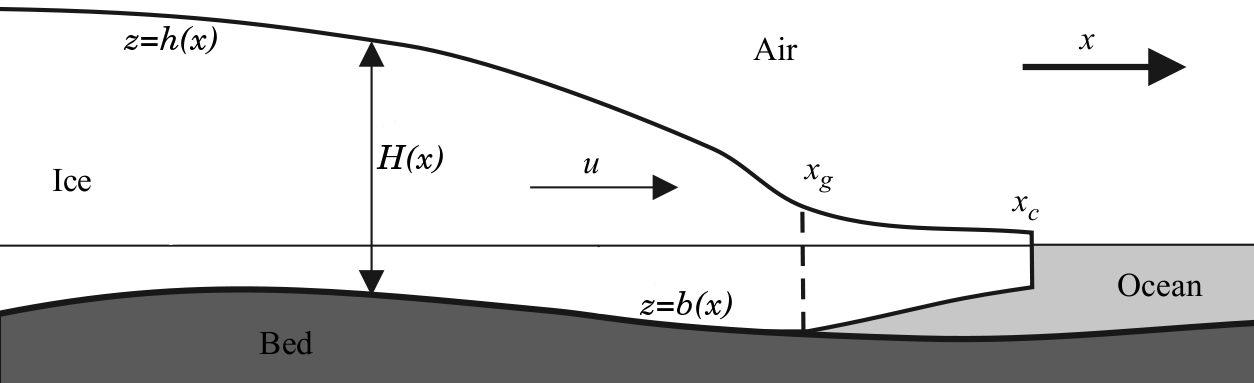
\includegraphics[width=6.0in]{flowline}
  
    \scriptsize \emph{Illustrates the notation used in these notes.  Figure modified from \cite{SchoofMarine1}.} \normalsize
    
    \vspace{1.5in}
  \end{center}
\end{titlepage}

\clearpage\newpage

%\setcounter{section}{1}
\section{Introduction}

The greatest importance of numerical models in glaciology is introspective.  You should ask yourself: When I combine my imperfect and incomplete understanding of glacier processes into this mathematical model which I put on a computer, does it behave as I expect?  Numerical models can indeed show how processes interact to give overall behavior.  They can at least demonstrate flaws in our understanding of those processes.  But they should be built with care.  An avoidable bad outcome is to spend time---or worse, reputation---interpreting, explaining, or justifying numerical model behavior that is in fact an artifact of poor computer programming or numerical analysis.

So the reader of these notes may be surprised that a continuum model, and not a computer code, seems to be our focus much of the time.  While all codes produce some numbers, we want numbers that actually come from the continuum model we have written down.  We will therefore analyse numerical implementations to see if they match the model equations and their solutions.

These notes have a limited scope:
  \begin{quote}\emph{shallow approximations of ice flow.}\end{quote}
They adopt a constructive approach; we provide:
  \begin{quote}\emph{example numerical codes that actually work.}\end{quote}
Within our scope are the shallow ice approximation (SIA) in two horizontal dimensions (2D), the shallow shelf approximation (SSA) in 1D, and the mass continuity and surface kinematical equations.  We recall the Stokes model, but we do not address its numerical solution.  Our numerical concepts include finite difference schemes, solving algebraic systems from stress balances, and the verification of codes using exact solutions.

Our notation, which generally follows \cite{GreveBlatter2009}, is common in the glaciological literature, but see Table \ref{tab:notation}.  Cartesian coordinates are $x,y,z$ with $z$ positive-upward.  If these coordinates or time $t$ appear as subscripts then they denote partial derivatives: $u_x = \partial u/\partial x$.  Tensor notation uses subscripts from the list $\{1,2,3,i,j\}$.  For example, ``$\tau_{ij}$'' or ``$\tau_{13}$'' denote entries of the deviatoric stress tensor.

These notes are based on nineteen Matlab codes, each about one-half page.  All have been tested in Matlab and Octave.  They are distributed by cloning the repository at
\begin{quote}
\url{https://github.com/bueler/mccarthy}
\end{quote}
\noindent and looking in the \texttt{mfiles/} subdirectory.  Five of these codes are printed here, with their comments stripped for compactness and clarity.  The electronic versions have generous comments and help files.

\begin{table}[ht]
\caption{Notation used in these notes, with values for some constants.}
\begin{tabular}{clll}
variable  & description & SI units & value \\
\hline
$A$ & $A=A(T)=$ ice softness in the Glen flow law & $\text{Pa}^{-n}\,\text{s}^{-1}$ \\
$B$ & ice hardness; $B=A^{-1/n}$ & $\text{Pa}\,\text{s}^{1/n}$ \\
$b$ & bedrock elevation & m \\
$c$ & specific heat in general & J kg$^{-1}$ K$^{-1}$ \\
$\nabla$ & (spatial) gradient & m$^{-1}$ \\
$\nabla\cdot$ & (spatial) divergence & m$^{-1}$ \\
$\mathbf{g}$ & gravity & m s$^{-2}$\phantom{foobar} & 9.81 \\
$H$ & ice thickness & m \\
$h$ & ice surface elevation & m \\
$\kappa$ & conductivity in general & J s$^{-1}$ m$^{-1}$ K$^{-1}$ \\
$M$ & climatic mass balance & m s$^{-1}$ \\
$n$ & exponent in Glen flow law & & 3 \\
$\nu$ & viscosity & Pa s \\
$p$ & pressure & Pa \\
$\bq$ & map-plane ice flux: $\bq = \int_{b}^{h} \bU\,dx = \bar{\bU} H$ & $\text{m}^2\,\text{s}^{-1}$ \\
$\rho$ & density of ice & kg m$^{-3}$ & 910 \\
$\rho_w$ & density of sea water & kg m$^{-3}$ & 1028 \\
$T$ & temperature & K \\
$\tau$ & norm (second invariant) of $\tau_{ij}$: $2 \tau^2 = \sum_{ij} \tau_{ij}^2$ & Pa \\
$\tau_{ij}$ & deviatoric stress tensor & Pa \\
$Du_{ij}$ & strain rate tensor & s$^{-1}$ \\
$\mathbf{U}$ & $=(u,v)$ horizontal ice velocity & m s$^{-1}$ \\
$\mathbf{u}$ & $=(u,v,w)$ 3D ice velocity & m s$^{-1}$ \\
\end{tabular}
\label{tab:notation}
\end{table}


\section{Ice flow equations}

My first goal in these notes is to get to an equation for which I can say:
\begin{center}
\emph{by numerically solving this equation, we have a usable model for an ice sheet.}
\end{center}
\noindent A ``usable'' model tends to be \emph{understood} as much as it is \emph{correct}.  Also, this first usable model will not be complete by any modern standard.  To get to my goal I first (briefly!) recall the continuum mechanical equations of ice flow.

Ice in glaciers is a moving fluid so we describe its motion by a velocity field $\mathbf{u}(t,x,y,z)$.  If the ice fluid were faster-moving than it actually is, and if it were linearly-viscous like liquid water, then it would be a ``typical'' incompressible fluid.  We would use the Navier-Stokes equations as the model:
\begin{align}
\nabla \cdot \mathbf{u} &= 0 &&\text{\emph{incompressibility}} \label{incompressible} \\
\rho \left(\mathbf{u}_t + \mathbf{u}\cdot\nabla \mathbf{u}\right) &= -\nabla p + \nabla \cdot (\nu \nabla \mathbf{u}) + \rho \mathbf{g} &&\text{\emph{stress balance}} \label{navierstokes}
\end{align}
In equation \eqref{navierstokes} the term $\mathbf{u}_t + \mathbf{u}\cdot\nabla \mathbf{u}$ is an acceleration.  The right-hand side of \eqref{navierstokes} is the total stress, and so equation \eqref{navierstokes} says ``$ma=F$'', i.e.~it is Newton's second law.  Much time has been spent to get partial understanding of the rich solutions of these Navier-Stokes equations; a book-length introduction like \cite{Acheson} is recommended.  The numerical solution of these equations is \emph{computational fluid dynamics} (CFD).

But, is ice flow modelling a part of CFD?  (And does a well-written general-purpose CFD text like \cite{Wesseling} help the glaciers student?)  It is true that ice sheet flow can be a large-scale fluid problem like atmosphere and ocean circulation in climate systems, but it is an odd one.  Consider some topics which might make ocean circulation modelling exciting, for example:
  \begin{center} turbulence \qquad convection \qquad  coriolis force  \qquad density stratification
  \end{center}
None of these topics are relevant to ice flow.  What could be interesting about the flow of slow, and surely boring, ice?

First observe that ice is indeed a slow fluid.  In terms of equation \eqref{navierstokes}, ``slow'' means $\rho \left(\mathbf{u}_t + \mathbf{u}\cdot\nabla \mathbf{u}\right) \approx 0$, which says that the forces (stresses) of inertia are negligible.  However, ice is also a shear-thinning fluid with a specific kind of nonlinearly-viscous (``non-Newtonian'') behavior in which larger shear strain rates imply smaller viscosity.  The viscosity $\nu$ in \eqref{navierstokes} is therefore not constant, and so we must separately state an empirically-based flow law in addition to restating \eqref{navierstokes} for slow flows.

\subsection*{Stokes equations}  The standard model for isothermal ice flow is this set of equations:
\begin{align}
\nabla \cdot \mathbf{u} &= 0 &&\text{\emph{incompressibility}} \label{incompressibleagain} \\
0 &= - \nabla p + \nabla \cdot \tau_{ij} + \rho \mathbf{g} &&\text{\emph{stress balance}} \label{forcebalance} \\
Du_{ij} &= A \tau^2 \tau_{ij} &&\text{\emph{$n$=3 Glen flow law}} \label{flowlaw}
\end{align}
In the flow law \eqref{flowlaw}, the deviatoric stress tensor $\tau_{ij}$ and the strain rate tensor $Du_{ij}$ appear; previous lectures cover these.  Here we merely note that: $Du_{ij} = (1/2)((u_i)_{x_j}+(u_j)_{x_i})$ if we index coordinates by $x_1,x_2,x_3=x,y,z$, each tensor in \eqref{flowlaw} is symmetric and has trace zero, and $\tau^2 = (1/2) \tau_{ij} \tau_{ij}$ (using the summation convention).

The Stokes equations do not contain a time derivative.  Thus boundary stresses, the force of gravity $\rho \mathbf{g}$, and ice softness $A$ together determine the velocity and stress fields (i.e.~$\bu$, $p$, $\tau_{ij}$) instantaneously.  Thus ice flow simulation codes have no memory of prior momentum or velocity.  Said another way, velocity is a ``diagnostic'' output of ice flow codes, because it is not needed for (re)starting a simulation.

\subsection*{Plane-flow Stokes equations}  Consider now the $x,z$-plane case of equations \eqref{incompressibleagain}, \eqref{forcebalance}, and \eqref{flowlaw}.  ``Plane-flow'' means that velocity component $v$ is zero and that all derivatives with respect to $y$ are zero:
\begin{align}
u_x + w_z &= 0 &&\text{\emph{incompressibility}} \label{incompressiblexz} \\
p_x &= \tau_{11,x} + \tau_{13,z} &&\text{\emph{stress balance} ($x$)} \label{stokespx} \\
p_z &= \tau_{13,x} - \tau_{11,z} - \rho g &&\text{\emph{stress balance} ($z$)} \label{stokespz} \\
u_x &= A \tau^2 \tau_{11} &&\text{\emph{flow law} (diagonal)}  \label{forceflowx} \\
u_z + w _x &= 2 A \tau^2 \tau_{13} &&\text{\emph{flow law} (off-diagonal)} \label{forceflowz}
\end{align}
Note that $\tau_{13}$ is a shear stress while $\tau_{11}$ and $\tau_{33}=-\tau_{11}$ are deviatoric longitudinal stresses.  Also $\tau^2 = \tau_{11}^2+\tau_{13}^2$ in this case.  Equations \eqref{incompressiblexz}--\eqref{forceflowz} form a system of five nonlinear equations in five scalar unknowns ($u,w,p,\tau_{11},\tau_{13}$).

\subsection*{Slab-on-a-slope}  Equations \eqref{incompressiblexz}--\eqref{forceflowz} are complicated enough to make us pause before jumping in to numerical solution methods, but  we can handle a simplified situation first.  A uniform slab of ice, or a ``slab-on-a-slope'', is both a case in which we can actually solve the Stokes equations, and a motivation for the shallow model in the next subsection.

\onefig{slab}{Rotated axes for a slab-on-a-slope flow calculation.}

We rotate our coordinates only for this example and not elsewhere in these notes.  The two-dimensional axes ($x$,$z$) shown in Figure \ref{fig:slab} are rotated downward (clockwise) at angle $\alpha>0$ so that the gravity vector has components $\mathbf{g} = (g \sin\alpha,- g \cos \alpha)$.  Equations \eqref{stokespx} and \eqref{stokespz} in these rotated coordinates are
\begin{align}
p_x &= \tau_{11,x} + \tau_{13,z} + \rho g \sin\alpha, \label{stokespxrot} \\
p_z &= \tau_{13,x} - \tau_{11,z} - \rho g \cos\alpha. \label{stokespzrot}
\end{align}
Assuming also that there is no variation with $x$, the whole set of Stokes equations \eqref{incompressiblexz}, \eqref{forceflowx}, \eqref{forceflowz}, \eqref{stokespxrot}, \eqref{stokespzrot} simplifies greatly:
\begin{align}
w_z &= 0 &   0 &= \tau_{11} \label{stokesslab} \\
\tau_{13,z} &= - \rho g \sin\alpha &   u_z &= 2 A \tau^2 \tau_{13} \notag \\
p_z &= -\tau_{11,z} = - \rho g \cos\alpha \notag
\end{align}
We apply boundary conditions for these functions of $z$: $w(0)=0$, $p(H)=0$, $u(0)=u_0$.  The basal velocity $u_0$ will remain undetermined for now.

By integrating equations \eqref{stokesslab} with respect to $z$, and using $\tau_{11}=0$, we get $w=0$, $p = \rho g \cos\alpha (H-z)$, and $\tau_{13} = \rho g \sin\alpha (H-z)$.  Note that $H-z$ is the depth below the ice surface, so both the pressure $p$ and shear stress $\tau_{13}$ are proportional to depth.  Because $u_z = 2 A \tau^2 \tau_{13}$, by integrating vertically again we find the horizontal velocity:
\begin{align}
u &= u_0 + \frac{1}{2} A (\rho g \sin\alpha)^3  \left(H^4 - (H-z)^4\right)  \label{uslab}
\end{align}

Do we believe formula \eqref{uslab}?  Figure \ref{fig:slabvel} compares it to observations of a mountain glacier, and it shows we have already done a credible job of capturing deformation flow velocity in this case.  We do not yet have a model for the sliding velocity $u_0$ (i.e.~basal motion).  

\twofigsizes{slabvel}{athabasca-deform}{Left:  Velocity from slab-on-a-slope formula \eqref{uslab}.  Right:  Inclinometry-measured velocity in a glacier (Athabasca Glacier \cite{SavagePaterson}).}{2.0in}{1.8in}

\subsection*{Plane-flow mass-continuity equation}  Observe that the equations so far do not address the change in shape of the glacier or ice sheet.  For this we need another equation, the \emph{mass continuity equation}.  We consider the general case of an $x,z$-plane flow with variable thickness and velocity, not just slab-on-a-slope.  Define the vertical average of the horizontal velocity:
	$$\bar U = \frac{1}{H}\int_0^{H} u\,dz.$$
The flux $q=\bar U\, H = \int_0^{H} u\,dz$ is the rate of flow input into the side of the area in Figure \ref{fig:slabmasscontfig}.

\onefigsize{slabmasscontfig}{Mass continuity equation \eqref{masscont1D} follows from considering the changing area $A$ of ice in a planar flow.  Ice can be added by surface mass balance $M$ or a difference of flux $q=\bar u H$ into the left and right sides.}{2.5in}

The ice area $A$ in Figure \ref{fig:slabmasscontfig} changes according to the sum of all the boundary contributions,
\begin{equation}
\frac{dA}{dt} = \int_{x_1}^{x_2} M(x)\,dx + \bar U_1 H_1 - \bar U_2 H_2: \label{masscontintegrated}
\end{equation}
Here $M(x)$ is the climatic mass balance at the ice surface.  (In three-dimensions, equation \eqref{masscontintegrated} would become an equation for $dV/dt$, the rate of change of ice volume.)

If the width $\Delta x=x_2-x_1$ is small then $A\approx \Delta x\, H$.  So we divide by $\Delta x$ and take $\Delta x \to 0$ in \eqref{masscontintegrated} and get
\begin{equation}
H_t = M - \left(\bar U H\right)_x \label{masscont1D}
\end{equation}
This mass continuity equation describes change in the ice thickness in terms of surface mass balance and ice velocity.  An important aspect of ice flow simulations is how one computes the velocity which goes into this equation.

\subsection*{Viscosity form of the flow law}  The flow law \eqref{flowlaw} has another form which we will use next, and also later in describing ice shelf and stream flow.  Recall $\tau^2 = (1/2) \tau_{ij} \tau_{ij}$ and also define $|Du|^2 = (1/2) Du_{ij} Du_{ij}$.  The scalars $\tau$ and $|Du|$ are norms (also ``second invariants'') of the tensors $\tau_{ij}$ and $Du_{ij}$, respectively.  By taking these norms of both sides of \eqref{flowlaw} we get $|Du| = A \tau^3$.  But then $\tau = A^{-1/3} |Du|^{1/3}$, so \eqref{flowlaw} can be rewritten
\begin{equation}
\tau_{ij} = 2 \nu\, Du_{ij}  \qquad \text{\emph{flow law (viscosity form)}} \label{viscosityflowlaw}
\end{equation}
where $\nu = (1/2) A^{-1/3} |Du|^{-2/3}$ is the nonlinear viscosity.  Often $B = A^{-1/3}$ is called the ice ``hardness''.  The derivation of \eqref{viscosityflowlaw} is worth knowing in detail; see the Exercises.

Form \eqref{viscosityflowlaw} of the flow law allows us to eliminate stresses $\tau_{ij}$ from the Stokes equations by replacing them with formulas depending on derivatives of the velocity.  That is, one can write the Stokes equations in terms of the strain rates only.  The next two approximate models also use this idea.

\subsection*{The Blatter-Pattyn approximation}  We return now briefly to plane-flow Stokes equations \eqref{incompressiblexz}--\eqref{forceflowz}, and reconsider how to simplify them.  One simplification step, present in all shallow models, is to drop the single term  $\tau_{13,x}$ from the $z$-component of the stress balance \eqref{stokespz}.  This assumes that horizontal variation in the vertical shear stress is small compared to the other terms:
\begin{equation}
p_z = - \tau_{11,z} - \rho g. \label{hydrostaticpz}
\end{equation}
Because the (Cauchy) stress tensor $\sigma_{ij}$ is related to the deviatoric stress tensor by $\sigma_{ij} = \tau_{ij} - p \delta_{ij}$, and thus $p + \tau_{11} = p - \tau_{33} = - \sigma_{33}$, equation \eqref{hydrostaticpz} says that the vertical normal stress $\sigma_{33}$ is linear in depth; this is similar to a statement that the ice is hydrostatic.  Taking it to have surface value zero we get
\begin{equation}
p + \tau_{11} = \rho g (h-z). \label{hydrostaticitself}
\end{equation}

Equation \eqref{hydrostaticitself} allows one to eliminate $p$ from the model equations.  Furthermore, taking the $x$-derivative of \eqref{hydrostaticitself} and substituting into \eqref{stokespx}, then using the viscosity form \eqref{viscosityflowlaw}, leads to this equation (Notes and References and \cite{GreveBlatter2009}):
\begin{equation}
\left(4 \nu u_x\right)_x + \left(\nu (u_z+w_x)\right)_z = \rho g h_x \qquad\text{\emph{hydrostatic stress balance}} \label{stresshydrostatic}
\end{equation}
The hydrostatic stress balance equation \eqref{stresshydrostatic} is nontrivially-coupled to incompressibility \eqref{incompressiblexz} because derivatives of the vertical velocity $w$ appear in both equations, though $p$ is gone.  Nonetheless coupled equations \eqref{incompressiblexz} and \eqref{stresshydrostatic}, along with the formula $\nu = (1/2) A^{-1/3} |Du|^{-2/3}$ and appropriate boundary conditions, determine $u$ and $w$.

If we drop $w_x$ from equation \eqref{stresshydrostatic} then we get the Blatter-Pattyn model:
\begin{equation}
\left(4 \nu u_x\right)_x + \left(\nu u_z\right)_z = \rho g h_x \qquad\text{\emph{Blatter-Pattyn stress balance}} \label{stressblatter}
\end{equation}
Using this equation one can solve first for the horizontal velocity $u$ and then afterward recover $w$ from \eqref{incompressiblexz}; stress balance and incompressibility are decoupled.

\section{Shallow ice sheets}

Ice sheets have four outstanding properties as fluids.  They are (\emph{i}) slow, (\emph{ii}) shallow,  (\emph{iii}) non-Newtonian, and (\emph{iv}) they experience some contact slip (basal sliding).  The first ice flow model which we solve numerically in these notes is the non-sliding, isothermal \emph{shallow ice approximation} (SIA).  It accounts for (\emph{i})--(\emph{iii}).

Regarding the property of shallowness, Figure \ref{fig:green-transect} shows both a no-vertical-exaggeration cross-section of Greenland at $71^\circ$, as well as the standard vertically-exaggerated version which is more familiar in the glaciological literature.  In other words, ice sheets \emph{are} shallow, though of course the portion of an ice sheet which you want to model may not be.

\onefig{green-transect}{A vertically-exaggerated cross-section of the Greenland ice sheet ($71^\circ$ N) is shown by the upper two curves.  Without exaggeration it appears as merely a thickened horizontal line.}

Our slab-on-a-slope example gives us a rough explanation of the SIA.  To show the SIA in its plane-flow form, we vertically integrate velocity formula \eqref{uslab} in the $u_0=0$ (non-sliding) case to get
\begin{equation}
\bar u H = \int_0^H \frac{1}{2} A (\rho g \sin\alpha)^3  \left(H^4 - (H-z)^4\right)\,dz = \frac{2}{5} A (\rho g \sin\alpha)^3 H^5. \label{siaubar}
\end{equation}
Note $\sin \alpha \approx \tan\alpha = - h_x$.  Combining these statements with mass continuity \eqref{masscont1D} gives
\begin{equation}
  H_t = M + \left(\frac{2}{5} (\rho g)^3 A H^5 |h_x|^2 h_x\right)_x. \label{sia1D}
\end{equation}

Equation \eqref{sia1D} is the SIA equation for nonsliding plane flow.  It is the promised first usable model for the evolution of an ice sheet's thickness $H$ in terms of surface mass balance $M$, ice softness $A$, and bed elevation $b$ (because $h=H+b$).  The model must, however, be solved subject to the constraint that the thickness is positive ($H\ge 0$); see Notes and References.

Additional arguments are needed to demonstrate that the SIA is more general-purpose than the special case of a simple slab; see Notes and References.  Such arguments reduce the Stokes equations under the assumption that the surface and bed slopes, and the depth-to-width ratio, are small.

We will numerically solve the SIA in section \ref{sec:numericalsia}, but first we state it in two horizontal dimensions.  Let $\mathbf{U} = (u,v)$ be the vector horizontal velocity.  The shear stress approximation is $(\tau_{13},\tau_{23}) \approx - \rho g (h-z) \nabla h$, which appeared as ``$\tau_{13}= \rho g \sin \alpha (h-z)$ and $\sin \alpha \approx -h_x$'' in the previous section, becomes an equality in the SIA.  Equation \eqref{flowlaw} then gives the SIA formula for shear strain rates
\begin{equation*}
\mathbf{U}_z = 2 A |(\tau_{13},\tau_{23})|^{n-1} (\tau_{13},\tau_{23}) = - 2 A (\rho g)^n (h-z)^n |\nabla h|^{n-1} \nabla h.
\end{equation*}
By integrating vertically we get, in the non-sliding case,
\begin{equation}
\mathbf{U} = - \frac{2 A (\rho g)^n}{n+1} \left[H^{n+1} - (h-z)^{n+1}\right] |\nabla h|^{n-1} \nabla h.  \label{siavelocity}
\end{equation}

Mass continuity in two horizontal dimensions, which generalizes the 1D version \eqref{masscont1D}, also applies:
\begin{equation}
    H_t = M - \Div\left(\bar{\mathbf{U}} H\right)  \label{masscont}
\end{equation}
Equation \eqref{masscont} may be written $H_t = M - \Div \bq$ in terms of the map-plane flux $\bq = \int_{b}^{h} \mathbf{U}\,dz = \bar{\mathbf{U}}\,H$.

Combining Equations \eqref{siavelocity} and \eqref{masscont}, we get an equation for the rate of thickness change in terms of mass balance $M$, thickness, and surface slope $\grad h$:
\begin{equation}
H_t = M + \Div \left(\Gamma H^{n+2} |\grad h|^{n-1} \grad h \right), \label{sia}
\end{equation}
where we have defined the positive constant $\Gamma = 2 A (\rho g)^n / (n+2)$.  Equation \eqref{sia} is the SIA in two dimensions.  Recalling our earlier promise, if we can solve \eqref{sia} numerically then we have, following Mahaffy \cite{Mahaffy}, a usable model for the Barnes ice cap in Canada, a particularly-simple ice sheet on a rather flat bed.

\subsection*{Analogy with the heat equation}  The SIA model is easy to compare with the better-known heat equation.  Numerical methods for solving \eqref{sia} can be understood as modifications of well-known heat equation methods.

In the simplest one-dimensional (1D) case, the heat equation for the temperature $T(t,x)$ of a conducting rod is
\begin{equation}
  T_t = D T_{xx}. \label{heat1D}
\end{equation}
This form applies when material properties are constant and there are no heat sources.  The positive constant $D$ is the ``diffusivity,'' with units which can be read from comparing sides of the equation: $D\sim \text{m}^2 \text{s}^{-1}$.  Observe that equation \eqref{heat1D} has a smoothing effect on the solution $T$ as it evolves in time, because any local maximum in the temperature is flattened (i.e.~$T_{xx}<0$ implies $T_t<0$ so $T$ decreases), while any local minimum is also flattened (i.e.~$T_{xx}>0$ implies $T_t>0$ so $T$ increases).

We will state the 2D heat equation more generally.  It describes the temperature $T(t,x,y)$ of some planar object, at position $x,y$ and time $t$.  Recall that Fourier's law for conduction is the formula $\mathbf{Q} = - \kappa \grad T$ for heat flux $\mathbf{Q}$, where $\kappa$ is conductivity.  We will assume, for the purposes of our analogy, that $\kappa(x,y)$ may vary in space.  Also suppose there is a variable heat source $f(t,x,y)$, with units of Watts per cubic meter.  Then conservation of internal energy says
\begin{equation}
\rho c T_t = f + \Div (\kappa \grad T). \label{heatearly}
\end{equation}
Here $\rho$ is density and $c$ is specific heat capacity.  Assuming $\rho c$ is constant, define the ``diffusivity'' $D=\kappa/(\rho c)$ and the rescaled source term $F = f/(\rho c)$.  The revised 2D heat equation is
\begin{equation}
T_t = F + \Div (D\, \grad T). \label{heat}
\end{equation}
It clearly generalizes equation \eqref{heat1D}.

Figure \ref{fig:initialheat} shows a solution of heat equation \eqref{heat}, wherein the initial condition is a localized ``hot spot''.  Solutions of the heat equation always involve the spreading, in all directions, of any local heat maxima or minima, that is, diffusion.

\twofigsizes{initialheat}{finalheat}{A solution of heat equation \eqref{heat} with $D=1$ and $F=0$.  Left: Initial condition $T(0,x,y)$.   Right: Solution $T(t,x,y)$ at $t=0.02$.}{2.8in}{2.8in}

The SIA equation \eqref{sia} and the heat equation \eqref{heat} are each diffusive, time-evolving partial differential equations (PDEs).  A side-by-side comparison is illuminating:
\begin{center}
\begin{tabular}{cc}
\vspace{1mm}
SIA:\, $H$ is ice thickness & \phantom{foo bar} heat: $T$ is temperature\phantom{foo bar}  \\
\vspace{1mm}
	$H_t = M + \Div \left({\color{red}\Gamma H^{n+2} |\grad h|^{n-1}}\, \grad h \right)$  &  $T_t = F + \Div (D\, \grad T)$
\end{tabular}
\end{center}
\vspace{1mm}
Notice that the number of derivatives (one time and two space derivatives) and the signs are the same.  Surface mass balance $M$ is analogous to heat source $F$.  

The analogy suggests that we identify the \emph{diffusivity in the SIA} as:
\begin{equation}
	D = {\color{red}\Gamma H^{n+2} |\grad h|^{n-1}}.  \label{siadiffusivity}
\end{equation}
A non-sliding SIA flow diffuses the thickness of the ice sheet, and when this $D$ comes out large then the diffusion acts most quickly.  Being a product of $\Gamma$ and the powers of $H$ and $|\grad h|$, this diffusivity $D$ is large if the ice is both thick and steep.  In summary, ice diffuses (i.e.~flows downhill) more when it is thick and steep.

This diffusion equation analogy explains generally why the surfaces of ice sheets are smooth, at least if we overlook non-flow processes like crevassing and wind-driven (snow) dunes.  There are, however, some practical and conceptual issues with the analogy:
\begin{itemize}
\item The diffusivity $D$ in \eqref{siadiffusivity} depends on the solution, both thickness $H$ and surface slope $|\grad h|$.  This affects how we reason about diffusivity.  Numerical solution processes are more difficult because nonlinear equations are harder to solve.
\item The diffusivity $D$ in \eqref{siadiffusivity} goes to zero at margins, where $H\to 0$, and at divides and domes, where $|\grad h|\to 0$.  This means that the solution is not smooth, even though the thickness is continuous everywhere (and zero outside the ice sheet).  A non-smooth solution generates larger numerical errors.
\end{itemize}
More important is a deficiency of the SIA model, and not the analogy \emph{per se}, namely
\begin{itemize}
\item Ice flow is much less diffusive when significant longitudinal (membrane) stresses are present, as when ice is floating or sliding or when the flow is confined by terrain.
\end{itemize}
Nonetheless we continue toward a verified numerical scheme for the SIA model \eqref{sia} (Section \ref{sec:numericalsia}).  The next Section introduces some numerical PDE methods in general.

\section{Finite difference numerics} 

The diffusivity analogy above suggests that numerical schemes for the heat equation are a starting point for solving the SIA equation \eqref{sia}.  Here we demonstrate only finite difference (FD) schemes, in which we replace derivatives by mere arithmetic.

The basic fact on which FD schemes are based is \emph{Taylor's theorem}, which says that for a smooth function $f(x)$,
	$$f(x+\Delta) = f(x) + f'(x) \Delta + \frac{1}{2} f''(x) \Delta^2 + \frac{1}{3!} f'''(x) \Delta^3 + \dots$$
You can replace ``$\Delta$'' by its multiples, for example:
\begin{align*}
f(x+2\Delta) &= f(x) + 2 f'(x) \Delta + 2 f''(x) \Delta^2 + \frac{4}{3} f'''(x) \Delta^3 + \dots \\
f(x-\Delta) &= f(x) - f'(x) \Delta + \frac{1}{2} f''(x) \Delta^2 - \frac{1}{3!} f'''(x) \Delta^3 + \dots
\end{align*}
The idea for constructing FD schemes is to combine expressions like these to give approximations of derivatives.  Thereby an equation relating values on a grid serves to approximate the differential equation.

Here we want partial derivative approximations, so we apply the Taylor's expansions one variable at a time.  For example, with a general function $u=u(t,x)$,
\begin{align*}
u_t(t,x) &= \frac{u(t+\Delta t,x) - u(t,x)}{\Delta t} + O(\Delta t), \\
u_t(t,x) &= \frac{u(t+\Delta t,x) - u(t-\Delta t,x)}{2\Delta t} + O((\Delta t)^2), \\
u_x(t,x) &= \frac{u(t,x+\Delta x) - u(t,x-\Delta x)}{2\Delta x} + O((\Delta x)^2), \\
u_{xx}(t,x) &= \frac{u(t,x+\Delta x) - 2\, u(t,x) + u(t,x-\Delta x)}{\Delta x^2} + O((\Delta x)^2)
\end{align*}
Note that if $\Delta$ is a small number then ``$+O(\Delta^2)$'' is smaller than ``$+O(\Delta)$'', so the approximation is closer when you drop it.

\subsection*{Explicit scheme for the heat equation}  We first build the simplest ``explicit'' scheme which approximates the 1D heat equation \eqref{heat1D}.  It is based on the fact that because $T_t$ and $D T_{xx}$ are equal, these two FD expressions are nearly equal:
\begin{equation}
\frac{T(t+\Delta t,x) - T(t,x)}{\Delta t} \approx D\,\frac{T(t,x+\Delta x) - 2\, T(t,x) + T(t,x-\Delta x)}{\Delta x^2}.  \label{heat1Dapproximated}
\end{equation}
The scheme itself is a method for computing numbers on a grid.  That is, \eqref{heat1Dapproximated} approximates the PDE, but making it into an equality tells how to \emph{determine} grid values.

Let $(t_n,x_j)$ denote the points of the time-space grid shown in Figure \ref{fig:timespacegrid}.  Denote our approximation of the solution value $T(t_n,x_j)$ by $T_j^n$.  Then the finite difference scheme is
	$$\frac{T_j^{n+1} - T_j^n}{\Delta t} = D\,\frac{T_{j+1}^n - 2\, T_j^n + T_{j-1}^n}{\Delta x^2}.$$
To get a computable formula, let $\mu = D \Delta t / (\Delta x)^2$ and solve for $T_j^{n+1}$:
\begin{equation}
  T_j^{n+1} = \mu T_{j+1}^n + (1 - 2 \mu) T_j^n + \mu T_{j-1}^n \label{heat1Dfd}
\end{equation}

\onefigsize{timespacegrid}{A grid for a finite difference solution to \eqref{heat1D}.}{2.0in}

FD scheme \eqref{heat1Dfd} is \emph{explicit} because it directly computes $T_j^{n+1}$ in terms of values at time $t_n$.  Figure \ref{fig:expstencil} (left) shows the ``stencil'' for scheme \eqref{heat1Dfd}: three values at the current time $t_n$ are combined to update the one value at the next time $t_{n+1}$.

Before moving on, notice that evaluating a heat equation solution at a grid point (i.e.~the expression ``$T(t_n,x_j)$'') is generally a different number from the value $T_j^n$ computed by a scheme like \eqref{heat1Dfd}.  We intend that the numbers $T(t_n,x_j)$ and $T_j^n$ become closer together as the grid is made finer (i.e.~$\Delta t \to 0$ and $\Delta x \to 0$), because the FD expressions become closer to the derivatives they approximate.  That is, we intend our FD scheme to \emph{converge} under \emph{grid refinement}.  For now we \emph{plan} and \emph{hope} that convergence happens, but it needs checking (``verification''; Section \ref{sec:exactsolutions}) or perhaps a proof.

\twofigsizes{expstencil}{exp2dstencil}{Left: Space-time stencil for the explicit scheme \eqref{heat1Dfd} for the 1D heat equation.  Right: Spatial-only stencil for scheme \eqref{heat2dexplicit}.}{2.0in}{2.1in}

How accurate is scheme \eqref{heat1Dfd}?  Its construction tells us that the difference between the scheme \eqref{heat1Dfd} and the PDE \eqref{heat1D} is $O(\Delta t + (\Delta x)^2)$, so this difference goes to zero as we refine the grid in space and time, a property called \emph{consistency}.  With care about the smoothness of boundary conditions, and using mathematical facts about the heat equation itself, one can show that the difference between $T_j^n$ and $T(t_n,x_j)$ is also $O(\Delta t + (\Delta x)^2)$, which is thus the \emph{convergence rate}; see Notes and References.

To get convergence the PDE problem must generate adequately smooth solutions, and also scheme \eqref{heat1Dfd} must be \emph{stable}, which we address below.  The main theorem for numerical PDE schemes is ``consistency plus stability implies convergence''; see Notes and References.  Instead of pursuing such theory, however, these notes we do something rather practical, namely verification.  We find problems for which we already know an exact solution $T(t,x)$, and then we compute the differences $|T_j^n - T(t_n,x_j)|$.  This determines directly whether our actual \emph{implementation} (i.e.~computer code form of the scheme) actually does converge, not just whether it should in theory.

\subsection*{A first implemented scheme}  Our first Matlab implementation is for the 2D Equation \eqref{heat} with $D$ constant and $F=0$:
\begin{equation}
T_t = D (T_{xx}+T_{yy}).\label{heat2D}
\end{equation}
Writing $T_{jk}^n \approx T(t_n,x_j,y_k)$, the 2D explicit scheme is
\begin{equation}
	\frac{T_{jk}^{n+1} - T_{jk}^n}{\Delta t} = D\,\left(\frac{T_{j+1,k}^n - 2\, T_{jk}^n + T_{j-1,k}^n}{\Delta x^2} + \frac{T_{j,k+1}^n - 2\, T_{jk}^n + T_{j,k-1}^n}{\Delta y^2}\right). \label{heat2dexplicit}
\end{equation}
The stencil for the right-hand side of \eqref{heat2dexplicit} is shown in Figure \ref{fig:expstencil} (right).

Scheme \eqref{heat2dexplicit} has implementation \texttt{heat.m} below.  For simplicity we set $T=0$ on the boundary of the square $-1 < x < 1$, $-1 < y < 1$.  The initial condition is gaussian: $T(0,x,y) = \exp(-30 (x^2+y^2))$.  The code uses Matlab ``colon'' notation to remove loops over spatial variables.  Here is an example run:
\begin{Verbatim}
>>  heat(1.0,30,30,0.001,20);
\end{Verbatim}
This sets $D=1.0$ and uses a $30\times 30$ spatial grid.  We take $N=20$ time steps of $\Delta t = 0.001$.  The result is shown in Figure \ref{fig:initialheat}, right.  This is the look of success.

\minput{heat}

However, very similar runs seem to succeed or fail according to some as-yet unclear circumstances.  For example, results from these calls are shown in Figure \ref{fig:stability}:
\begin{Verbatim}
>> heat(1.0,40,40,0.0005,100);    % Figure 8, left
>> heat(1.0,40,40,0.001,50);      % Figure 8, right
\end{Verbatim}
Both runs compute temperature $T$ on the same spatial grid, for the same final time $t_f = N \Delta t = 0.05$, but with different time steps.  Noting the vertical axes, the second run clearly shows ``instability,'' an extreme form of inaccuracy characterized in practice by numbers of a totally different magnitude than expected.

\twofig{stability}{instability}{Numerically-computed temperature on $40\times 40$ grids.  The two runs are the same except that the left has $\Delta t=0.0005$ so $D\Delta t/(\Delta x)^2= 0.2$, while the right has $\Delta t=0.001$ so $D\Delta t/(\Delta x)^2= 0.4$.  Compare \eqref{stabcrit}.}


\subsection*{Stability criteria and adaptive time stepping}  To avoid the instability shown at right in Figure \ref{fig:stability}, we need to understand the scheme better.  It turns out we have not made an implementation error.  Instead, care is required when choosing space and time steps.

Recall the 1D explicit scheme in form \eqref{heat1Dfd}: $T_j^{n+1} = \mu T_{j+1}^n + (1 - 2 \mu) T_j^n + \mu T_{j-1}^n$.  The new value $T_j^{n+1}$ is an average of the old values, in the sense that the coefficients add to one.  Averaging is stable because averaged wiggles are smaller than the wiggles themselves.  Actually, however, the scheme is only an average \emph{if} the middle coefficient is positive, as a linear combination with coefficients which add to one is not an average if any coefficients are negative.  (For example, one would not accept 15 as an ``average'' of 5 and 7, but: $15 = -4 \times 5 + 5 \times 7$, and $-4+5=1$.)

So, what follows from requiring the middle coefficient in \eqref{heat1Dfd} to be positive so it computes such an average?  A \emph{stability criterion} follows, with these equivalent forms:
\begin{equation}
   1 - 2 \mu \ge 0 \quad \iff \quad \frac{D\Delta t}{\Delta x^2} \le \frac{1}{2} \quad \iff \quad \Delta t \le \frac{\Delta x^2}{2 D}.  \label{stabcrit}
\end{equation}
The third form states the condition as a limitation on the size of $\Delta t$.  It is a \emph{sufficient} stability criterion; it is enough to guarantee stability, though something weaker might do.  In summary, for given $\Delta x$, shortening the time steps $\Delta t$ so that \eqref{stabcrit} holds will make FD scheme \eqref{heat1Dfd} into an averaging process.

Applying this same idea to the 2D heat equation \eqref{heat2D} leads to the stability condition that $1-2\mu^x-2\mu^y \ge 0$ where $\mu^x = D \Delta t / (\Delta x^2)$ and $\mu^y = D \Delta t / (\Delta y^2)$.  In the cases shown in Figure \ref{fig:stability}, wherein $\Delta x=\Delta y$, this condition requires $D \Delta t /(\Delta x^2) \le 0.25$.  This inequality precisely distinguishes between the two parts of Figure \ref{fig:stability}.

In summary, runs of \texttt{heat.m} are unstable if the time step $\Delta t$ is too big relative to the spacing $\Delta x$.  The stability criterion is, however, satisfied by making each time step shorter.  Enforcing the criterion inside the code itself is an \emph{adaptive} implementation.  Such an implementation can be stable even if the diffusivity $D$ is changing in time.  To show how easy this is to implement, \texttt{heatadapt.m} (not shown) is the same as \texttt{heat.m} except that the time step comes from the stability criterion.  However, if the diffusivity $D$ is large or the grid spacings $\Delta x$, $\Delta y$ are small, then adaptive explicit implementations must take many short time steps to assure stability.  Adaptive explicit schemes can be slow.


\subsection*{Implicit schemes}  There is an alternative stability fix instead of adaptivity, namely ``implicitness.''  For example, the finite difference scheme
\begin{equation}
  \frac{T_j^{n+1} - T_j^n}{\Delta t} = D\,\frac{T_{j+1}^{n+1} - 2\, T_j^{n+1} + T_{j-1}^{n+1}}{\Delta x^2} \label{implicit1D}
\end{equation}
is an $O(\Delta t + (\Delta x)^2)$ implicit scheme for Equation \eqref{heat1D}.  This implicit scheme for the heat equation is stable for \emph{any} positive time step $\Delta t>0$ (``unconditionally stable''); see Notes and References.  Another well-known implicit scheme is \emph{Crank-Nicolson}, which is unconditionally stable for the heat equation, but with smaller error $O((\Delta t)^2 +(\Delta x)^2)$.

Implicit schemes are harder to implement because the unknown solution values at time step $t_{n+1}$ are treated as a vector in a large system of equations which must be formed and solved at each time step.  If the PDE is nonlinear then the system of equations may be hard to solve.  Though the SIA is a highly nonlinear diffusion equation, implicit schemes are becoming useful \cite{Bueler2016}.  Because of the tradeoff between the easy implementability of adaptive explicit schemes and the better stability of implicit schemes, for these notes we stay with adaptive explicit (FD) schemes.

\subsection*{Numerical solution of diffusion equations}  We are trying to numerically model ice flows, not heat conduction.  We have an analogy, however, which says that the SIA is diffusive like the heat equation.  In this section, because we wish to solve the SIA on real bedrock, we construct a numerical scheme for a more general diffusion equation which has an extra ``shift'' inside the gradient, namely
\begin{equation}
  T_t = F + \Div \left(D \grad (T + b)\right). \label{gendiffusion}
\end{equation}
In equation \eqref{gendiffusion}, the source term $F(x,y)$, the diffusivity $D(x,y)$, and the ``shift'' $b(x,y)$ may all vary in space.

The following code solves \eqref{gendiffusion}.  It is called by the SIA-specific schemes we build next.

\minput{diffusion}

This adaptive explicit method for the diffusion equation is conditionally stable, with the same essential time step restriction as for the constant diffusivity case, as long as we evaluate $D(x,y)$ at \emph{staggered} grid points.  That is, we use this expression for the second derivative:
\begin{align*}
\Div \left(D \grad X\right) &\approx \frac{D_{j+1/2,k}(X_{j+1,k} - X_{j,k}) - D_{j-1/2,k}(X_{j,k} - X_{j-1,k})}{\Delta x^2} \\
	&\qquad + \frac{D_{j,k+1/2}(X_{j,k+1} - X_{j,k}) - D_{j,k-1/2}(X_{j,k} - X_{j,k-1})}{\Delta y^2},
\end{align*}
where $X=T+b$.  The left part of Figure \ref{fig:diffstencil} shows the stencil.

\twofigsizes{diffstencil}{mahaffystencil}{Left:  Spatial stencil for staggered grid evaluation of diffusivity (at triangles) in the diffusion equation \eqref{gendiffusion}.  Right: Stencil showing how the staggered-grid diffusivity (triangle) can be evaluated in the SIA, from surface elevation (diamonds) and thicknesses (squares).}{2.2in}{2.2in}

The user supplies the diffusivity $D(x,y)$ to \texttt{diffusion.m} on the staggered grid.  The initial temperature $T(0,x,y)$, source term $F(x,y)$, and ``shift'' $b(x,y)$ are also supplied on the regular grid.  When using this code for standard diffusions, or for the flat-bed case of the SIA, we would take $b=0$.


\section{Numerically solving the SIA} \label{sec:numericalsia}

In SIA equation \eqref{sia} we have diffusivity $D = \Gamma H^{n+2} |\grad h|^{n-1}$.  As already noted, an interesting aspects of this formula is that $D$ goes to zero, the diffusion ``degenerates,'' when either $H\to 0$ or $\grad h \to 0$.  Degenerate diffusion equations are automatically free boundary problems, but this aspect of the thickness evolution problem should be no surprise to a glaciologist.  Determining the location of the margin is an obvious part of modelling a glacier or ice sheet.  To address this free boundary issue in our explicit time-stepping code it suffices to numerically compute new thicknesses and then set them to zero if they come out negative.

Second, for numerical stability and mass conservation we should compute $D$ on a ``staggered'' grid.  Various finite difference schemes for computing it have been proposed.  All of these schemes involve averaging $H$ and differencing $h$ in a ``balanced'' way onto the staggered grid.  In the code \texttt{siaflat.m} below we use the Mahaffy \cite{Mahaffy} method, with the stencil for computing $D$ shown in Figure \ref{fig:diffstencil} (right).  This code only works for the flat bed, zero surface mass balance case, but we will correct these deficiencies later.

\minput{siaflat}


\section{Exact solutions and verification} \label{sec:exactsolutions}

In \texttt{siaflat.m}, which calls \texttt{diffusion.m}, we already have a fairly complicated code.  How do we make sure that such an implemented numerical scheme is correct?  Here are three proposed techniques:
\begin{enumerate}
  \item don't make any mistakes, or
  \item compare your numerical results with results from other researchers, and hope that the outliers are in error, or
  \item compare your numerical results to an exact solution.   \end{enumerate}
The first two of these, which one might call ``infallibility'' and ``intercomparison,'' respectively, should be less common approaches than they are.  The last one of these, preferred to the first two by the CFD community generally \cite{Wesseling}, is called ``verification.''

It is a simple idea:  When we build a new computer code we should test it in cases where we know the right answer.  To do so we need to return to the PDE itself, to get useful exact solutions.

\subsection*{Exact solution of heat equation}  First we return to the simpler case of the 1D heat equation with constant $D$, namely $T_t = D T_{xx}$.  Many exact solutions $T(t,x)$ to this heat equation are known, but let's consider the time-dependent ``Green's function,'' also known as the ``heat kernel''.  It starts at time $t=0$ with a delta function $T(0,x)=\delta(x)$ of heat at the origin $x=0$.  Then it spreads out over time.  It is a solution of the heat equation on the whole line $-\infty<x<\infty$ and for all $t>0$.

We will calculate this exact solution by a method which generalizes to the SIA.  In both cases the Green's function is ``self-similar'' over time, in the sense that it changes shape \emph{only} by shrinking the output (vertical) axis and lengthening the input (horizontal) axis, as shown in Figure \ref{fig:heatscaling} for the heat equation.  These scalings are related to each other by conservation of energy, which says that the total heat energy is independent of time.

\onefigsize{heatscaling}{The heat equation Green's function in 1D has the same shape at each time, but with time-dependent input- and output-scalings.}{2.4in}

The Green's function of the 1D heat equation is
  $$T(t,x) = (4 \pi D t)^{-1/2}\, e^{-x^2/(4Dt)}.$$
``Similarity'' variables for this solution, the above-mentioned scalings, involving multiplying the input and output of an invariant shape function $\phi(s) = (4 \pi D)^{-1/2}\, e^{-s^2/(4D)}$ by the same power of $t$:
\begin{equation}
s \stackrel{\text{\emph{input scaling}}}{\phantom{\Big|}=\phantom{\Big|}} t^{-1/2} x, \qquad\qquad T(t,x) \stackrel{\text{\emph{output scaling}}}{\phantom{\Big|}=\phantom{\Big|}} t^{-1/2} \phi(s).  \label{heatscalings}
\end{equation}

A numerical solver for the 1D heat equation which starts with initial values $T(t_0,x)$ taken from this exact solution should, at a later time $t$, produce numbers which are close to the exact solution $T(t,x)$; see the Exercises.

\subsection*{Halfar's similarity solution to the SIA}  Now we jump from Green's idea in about 1830 to the year 1981.  That is when P.~Halfar published the similarity solution of the SIA in the case of flat bed and zero surface mass balance.  Halfar's solution to the 2D SIA model \eqref{sia}, using a Glen exponent $n=3$, has scalings similar to \eqref{heatscalings} above:
\begin{equation}
s = t^{-1/18} r, \qquad \qquad H(t,r)=t^{-1/9} \phi(s). \label{halfarscalings}
\end{equation}
Here $r=(x^2+y^2)^{1/2}$ is the distance from the origin.  These scalings are related to each other by conservation of mass, because no mass is gained or lost through the surface. Scalings \eqref{halfarscalings} imply that, quite differently from heat, the diffusion of ice slows down severely as the shape flattens out.  Said directly, the powers $t^{-1/9}$ and $t^{-1/18}$ change very slowly for large times $t$.

\onefigsize{siascaling}{Radial sections of Halfar's solution \eqref{halfar} of the SIA equation \eqref{sia} on a flat bed with zero mass balance.  The solution is shown on $H$ (m) versus $r$ (km) axes for times $t=1,10,100,1000,10000$ years.}{5.5in}

The formula for the Halfar solution to the SIA is remarkably simple given all that it accomplishes:
\begin{equation}
H(t,r) = H_0 \left(\frac{t_0}{t}\right)^{1/9} \left[1 - \left(\left(\frac{t_0}{t}\right)^{1/18} \frac{r}{R_0}\right)^{4/3}\right]^{3/7}. \label{halfar}
\end{equation}
Here the ``characteristic time'' $t_0 = (18 \Gamma)^{-1} (7/4)^3 R_0^4 H_0^{-7}$ is a parameter which can be determined by choosing center height $H_0$ and radius $R_0$.

Formula \eqref{halfar} is plotted in Figure \ref{fig:siascaling}.  We see that for times significantly greater than $t_0$ (i.e.~$t/t_0 \gg 1$) the solution changes very slowly.  For example, the change between years $1$ and $100$ is larger than that between years $1000$ and $10000$.  The \emph{volume} of ice is, however, constant with $t$; see the Exercises.

\subsection*{Using Halfar's solution}  Formula \eqref{halfar} is simple enough to use for verifying time-dependent SIA models.  The code \texttt{verifysia.m} (not shown) takes as input the number of grid points in each ($x,y$) direction.  It uses the Halfar solution at 200 a as the initial condition, does a numerical run of \texttt{siaflat.m} above to a final time 20000 a, and then compares to the Halfar formula for that time.  By ``compares'' we mean it computes the thickness \emph{numerical error}, the absolute values of the differences between the numerical and exact thickness solutions at the final time:
\small
\begin{verbatim}
>> verifysia(20)
average thickness error     = 22.310
>> verifysia(40)
average thickness error     = 9.490
>> verifysia(80)
average thickness error     = 2.800
>> verifysia(160)
average thickness error     = 1.059
\end{verbatim}
\normalsize
We see that the average thickness error decreases with increasing grid resolution.  This is as expected for a correctly-implemented code.  What is less obvious, perhaps, is that almost any numerical implementation mistake---almost any bug---will break this property, and these errors will not shrink.

You might ask, is the Halfar solution ever useful for modelling real ice masses?  The answer is yes.  In fact, J.~Nye and others (2000; \cite{NyeIcarus2000}) compared the long-time consequences of different flow laws for the south polar cap on Mars.  In particular, they evaluated $\text{CO}_2$ ice and $\text{H}_2\text{O}$ ice softness parameters by comparing the long-time behavior of the corresponding Halfar solutions to the observed polar cap properties.  Their conclusions:
  \begin{quote}
  \dots none of the three possible [$\text{CO}_2$] flow laws will allow a 3000-m cap, the thickness suggested by stereogrammetry, to survive for $10^7$ years, indicating that the south polar ice cap is probably not composed of pure $\text{CO}_2$ ice [but rather] water ice, with an unknown admixture of dust.
  \end{quote}
This theoretical result has since been confirmed by the observation and sampling of the polar geology of Mars.

Are exact solutions like Halfar's always available when needed?  The answer is ``no'', of course, though many ice flow models do have exact solutions which are relevant to verification; see the Notes and References.  For example, we will use van der Veen's solution for ice shelves in a later section.  On the other hand, the absence of exact solutions may show that not enough thought has gone into the continuum model itself.

\subsection*{A test of robustness}  Verification is an ideal way to start testing a code.  Another kind of test is for ``robustness'' over unusual or difficult input cases.  One asks: Does the model break?  In a robustness test one does not have precise knowledge of what the code \emph{should} do, but it is a useful test if we can at least identify obviously-unreasonable outputs.

The robustness test in the program \texttt{roughice.m} (not shown) demonstrates that \texttt{siaflat.m} can handle an ice sheet with extraordinarily large ``driving stresses.''  Recall that glaciological driving stress is $\tau_d = - \rho g H \grad h$.  This quantity appears in the slab-on-a-slope example, and thus in the SIA model, as the value of the shear stress $(\tau_{13},\tau_{23})$ at the base of the ice.  The driving stress is, obviously, large when the ice is both thick and has steep surface slope $|\nabla h|$.

\twofigsizes{roughinitial}{roughfinal}{The SIA model evolves the huge-driving-stress initial ice sheet at left to the ice cap at right in only 50 model years.}{2.9in}{2.9in}

In \texttt{roughice.m} we give \texttt{siaflat.m} a randomly-generated initial ice sheet which is of the worst possible sort because it is thick (average of 3000 m) \emph{and} it has large surface slopes.  The product $H|\grad h|$ is therefore large everywhere.  The initial shape is shown in the left side of Figure \ref{fig:roughinitial}.  During the run of 50 model years on a 17 km grid, the time step is determined adaptively from \eqref{stabcrit}.  The maximum diffusivity $D$ decreases over the course of the run, as the surface becomes smooth through flow, and thus the time-step increases from about 0.0002 years to 0.2 years.  The maximum value of the driving stress decreases from $57$ bar ($= 5.7\times 10^6$ Pa) to $3.6$ bar.  At the end of the run the ice cap has the shape shown at right in Figure \ref{fig:roughinitial}.

The shape at right in Figure \ref{fig:roughinitial} is rather close to a Halfar solution \eqref{halfar}.  Halfar essentially proved that \emph{all} solutions of the zero-mass-balance SIA on a flat bed asymptotically approach \eqref{halfar}; the Halfar solution is generic and attracting.


\section{Application to the Antarctic ice sheet}

Finally we apply the model to the Antarctic ice sheet.  To do this we must first modify \texttt{siaflat.m} to allow non-flat bedrock elevation $b(x,y)$ and arbitrary surface mass balance $M(x,y)$, and we enforce non-negative thickness at each timestep.  (In other words, we must complete the mass-continuity part of the model, whereas we have already tested the flow part.)  Also we add a minimal model of interaction with the ocean, namely we calve-off any ice that satisfies the flotation.  The result is \texttt{siageneral.m} (not shown), a code only ten lines longer than \texttt{siaflat.m}.

\twofigsizes{antinitial}{antfinal}{Left: Initial surface elevation (m) of Antarctic ice sheet.  Right: Final surface elevation at end of 40 ka model run on 50 km grid.}{2.55in}{3.2in}

We use measured accumulation, bedrock elevation, and surface elevation from ALBMAPv1 data \cite{LeBrocqetal2010}.  Melt is not modelled so the climatic mass balance is equal to the precipitation rate, clearly a more-suitable approximation for Antarctica than for Greenland, for example, but still a rough approximation.  These input data are read from a NetCDF file and preprocessed by an additional code \texttt{buildant.m} (not shown).

\onefig{antvolcompare}{Ice volume of the modeled Antarctic ice sheet, in units of $10^6 \, \text{km}^3$, from runs on 50 km (red), 25 km (green), and 20 km (blue) grids.}

The code \texttt{ant.m} (not shown) calls \texttt{siageneral.m} to do the simulation in blocks of 500 model years.  The volume is computed at the end of each block.  Figure \ref{fig:antinitial} shows the initial and final surface elevations from a run of 40,000 model years on a $\Delta x = \Delta y = 50$ km grid.  The runtime on a typical laptop is a few minutes.

Areas of the Antarctic ice sheet with low-slope and (actual) fast-flowing ice experience thickening in the model, while near-divide ice in East Antarctica, in particular, thins.  Assuming the present-day Antarctic ice sheet is somewhere near steady state, we can see that these thickness differences reflect model inadequacies.  The lack of a sliding mechanism explains the thickening in low-slope areas.  The lack of thermomechanical coupling, or equivalently the constancy of ice softness, and the fact that our isothermal $A$ value is quite ``soft'', explains the thinning near the divide; see Notes and References on modelling techniques which address these inadequacies.

We should be modelling floating ice too, but the SIA is completely inappropriate to that purpose.  Floating ice is addressed in section \ref{sec:shelvesandstreams}

Figure \ref{fig:antvolcompare} compares the ice volume time series for 50 km, 25 km, and 20 km grids.  This result, namely grid dependence of the ice volume, is typical.  One cause is that most steep gradients near the ice margin are poorly resolved, but to differing degrees at these coarse resolutions.  Figure \ref{fig:antvolcompare} is a warning about the interpretation of model runs:  Even if the data is available only on a fixed grid, the model should be run at different resolutions to evaluate the robustness of the model results.


\section{Mass continuity and kinematical equations}

Recall that in the SIA the stress balance becomes formula \eqref{siavelocity} for the velocity, which combines with the mass continuity equation \eqref{masscont} to give model \eqref{sia} for evolution of the ice sheet thickness.  The SIA equation \eqref{sia} therefore combines two concepts which we will now think about separately, and in greater generality, in the remainder of these notes.

The most basic shallow assumption made by most ice flow theories\footnote{There are several inequivalent shallow theories: SIA, SSA, hybrids, Blatter-Pattyn, \dots} is that the surface and base of the ice are differentiable functions $z=h(t,x,y)$ and $z=b(t,x,y)$.  Thus surface overhang is not allowed.  Though the Stokes theory allows the fluid boundary to be a closed surface in three-dimensional space, ice sheet and glacier models take a map-plane perspective and have a well-defined ice thickness: $H=h-b$.

To pursue such ideas a bit further, let us state the ``kinematical equations'' which apply at upper and lower surfaces of the ice sheet.  Let $a$ be the (upper surface) climatic mass balance function ($a>0$ is accumulation) and $s$ be the basal melt rate function ($s>0$ is basal melting).  In the equations which follow these are measured in thickness-per-time units, but they could be in mass-per-area-per-time units also.  The net map-plane mass balance $M=a-s$, which appears in the mass continuity equation \eqref{masscont}, is the difference of these surface fluxes.

The \emph{(upper) surface kinematical equation} is 
\begin{equation}
h_t = a - \mathbf{U}\big|_h \cdot \grad h + w\big|_h,  \label{surfkine}
\end{equation}
and the \emph{base kinematical equation} is
\begin{equation}
b_t = s - \mathbf{U}\big|_b \cdot \grad b + w\big|_b.  \label{basekine}
\end{equation}
wherein $\mathbf{U}$ is the horizontal ice velocity and $w$ the vertical ice velocity.  Equations \eqref{surfkine} and \eqref{basekine} describe the movement of the ice's upper surface and lower surfaces, respectively, from the velocity of the ice and the mass balance functions at the respective surfaces.

We can now state an important mathematical fact which follows from the assumption of well-defined upper and basal surface elevations and from incompressibility.  Namely, that the surface kinematical and mass continuity equations are closely-related.  More precisely, any pair of these equations implies the third:
  \begin{itemize}
  \item the surface kinematical equation \eqref{surfkine},
  \item the base kinematical equation \eqref{basekine}, and
  \item the map-plane mass continuity equation \eqref{masscont}.
  \end{itemize}
One proves these facts by using equation \eqref{incompressible} and the Leibniz rule for differentiating integrals.  The details are left for exercises.

The bedrock is often regarded as fixed (i.e.~$b_t=0$).  In the important (and idealized) case of non-deformable bedrock and no sliding, \eqref{basekine} says that the basal value of the vertical velocity equals the basal melt rate: $w\big|_b=-s$.

\subsection*{Prognostic models}  We can now sketch the structure of a general, explicit, ``prognostic,'' i.e.~ice geometry evolving, isothermal ice sheet model.  Each time step follows this recipe:
  \begin{itemize}
  \item numerically solve a stress balance, which gives velocity $\mathbf{u}=(u,v,w)$,
    \begin{itemize}
    \item[$\circ$] the geometry of the ice mass and the stress boundary conditions determine $\mathbf{u}$
    \item[$\circ$] if the stress balance only gives $\mathbf{U}=(u,v)$, get $w$ from incompressibility \eqref{incompressible},
    \end{itemize}
  \item decide on a time step $\Delta t$ for \eqref{masscont} based on velocities and/or diffusivities,
  \item from the horizontal velocity $\mathbf{U}=(u,v)$, compute the flux $\bq = \bar{\bU} H$,
  \item update mass balance $M=a-s$ and do a time-step of \eqref{masscont} to get $H_t$,
  \item update the upper surface elevation and thickness (e.g.~$h \mapsto h + H_t \Delta t$), and repeat.
  \end{itemize}
Like most ice sheet models, we use the mass continuity equation \eqref{masscont} to describe changes in ice sheet geometry, but we could use the surface kinematical equation \eqref{surfkine} instead.

The above ``standard'' ice sheet model has many variations.  Some glaciological questions are answered just by solving the stress balance for the velocity.  Sometimes the goal is the steady state configuration of the glacier.  This may be computed more quickly than via physical time-stepping physical evolution equations to steady state, but the thickness-positive constraint then, necessarily, becomes a focus of the analysis \cite{Bueler2016,JouvetBueler2012}.  Other processes are usually simulated at each time step, such as the conservation of energy within the ice, or subglacial and supraglacial processes.  Understanding the diverse time scales associated to these processes is always an important step in designing a model which is more complete than the isothermal SIA.

When using the SIA equation \eqref{sia}, one can apparently bypass the computation of the velocity.  That is because the mass continuity equation can be written as a diffusion, with $\bq=-D\nabla h$ for the flux, instead of with the more general formula $\bq = \bar{\bU} H$.  Fast flow in ice sheets is associated with sliding and floating ice, however, and for these flows the ice geometry evolution is not a diffusion.  While the formula $\bq = \bar{\bU} H$ applies, both for the SIA and fast flow, an ice flow model is also not hyperbolic.  Fundamentally, that is because the velocity is related to the local surface gradient.  In any case, solving the stress balance for the velocity field is generally a nontrivial and obligatory step in a numerical ice flow model.  We get started on one such case in the next Section.


\section{Shelves and streams} \label{sec:shelvesandstreams}

As its name suggests, the shallow shelf approximation (SSA) stress balance applies to ice shelves.  The SSA also applies reasonably well to ice streams which have not-too-steep bed topography and low basal resistance, like those in Figure \ref{fig:siple}.

\twofigsizes{siple}{streamisbrae}{Left:  The SSA model applies to ice streams like these on the Siple Coast in Antarctica.  Color shows radar-derived surface speed.  Right: Cross sections, \emph{without} vertical exaggeration, of (\textbf{a}) the Jakobshavns Isbrae outlet glacier in Greenland and (\textbf{b}) the Whillans Ice Stream on the Siple Coast \cite{TrufferEchelmeyer}.}{2.8in}{2.9in}

But what is, and is not, an ice stream?  Ice streams slide at $50$ to $1000 \,\text{m}\,\text{a}^{-1}$, they have a concentration of vertical shear in a thin layer near base, and typically they flow into ice shelves.  Pressurized liquid water at their beds plays a critical role enabling their fast flow.  There are other fast-flowing grounded parts of ice sheets, however, called ``outlet glaciers''.  They can have even faster surface speed (up to $10 \,\text{km}\,\text{a}^{-1}$), but it is typically uncertain how much of this speed is from sliding at the base.  In an outlet glacier there is substantial vertical shear ``up'' in the ice column, sometimes caused by soft temperate ice in a significant fraction of the thickness.  Furthermore, outlet glaciers are strongly controlled by fjord-like, large-slope bedrock topography.  Figure \ref{fig:siple} (right) compares the shallowness and bedrock topography of an outlet glacier and an ice stream.  Few simplifying assumptions are appropriate for outlet glaciers, and the SSA may not be a sufficient model.

\subsection*{The shallow shelf approximation (SSA)}  We state this stress balance equation only in the plane flow (``flow-line'') and isothermal case:
\begin{equation}
  \left(2 B H |u_x|^{1/n - 1} u_x\right)_x - C|u|^{m-1}u = \rho g H h_x \label{ssaearly}
\end{equation}
The term in parentheses is the vertically-integrated longitudinal stress.  (It is called the ``membrane'' stress when there are two horizontal dimensions.)  The second term $\tau_b = - C|u|^{m-1}u$ is the basal resistance, which is zero (i.e.~$C=0$) in an ice shelf.  The term on the right is the negative of the driving stress ($\tau_d = - \rho g H h_x$).  Thus the longitudinal strain rates are determined by the integrated ice hardness (i.e.~the coefficient $BH$), the slipperyness of the bed (i.e.~by the coefficient $C$ and the power $m$) and the geometry of the ice sheet (i.e.~the thickness $H$ and the surface slope $h_x$).  The power-law formula for the basal resistance $\tau_b$ is often called a ``sliding law.''

In \eqref{ssaearly} the velocity $u$ is independent of the vertical coordinate $z$.  We assume that the ice hardness $B=A^{-1/n}$ is also independent of depth.  Models which are not isothermal must compute the vertical average of the temperature-dependent hardness.  In any case the coefficient $\bar \nu = B |u_x|^{1/n-1}$ is the ``effective viscosity'', and \eqref{ssaearly} can be written
\begin{equation}
  \left(2 \,\bar \nu\, H u_x\right)_x - C |u|^{m-1} u = \rho g H h_x.  \label{ssa}
\end{equation}
In form \eqref{ssa} it must be understood that the viscosity $\bar\nu$ depends on $u$.

The inequality ``$\,\rho H < - \rho_w b\,$'' is called the \emph{flotation criterion}.  For grounded ice $\rho H > - \rho_w b$ holds, in which case the driving stress $\tau_d$ uses $h = H+b$.

Floating ice satisfies $\rho H < - \rho_w b$, and $h = (1-\rho/\rho_w) H$ is used in the driving stress.  Equation \eqref{ssa} therefore simplifies if the ice is floating:
\begin{equation}
   \left(2 \,\bar\nu\, H u_x\right)_x = \rho g (1-\rho/\rho_w) H H_x. \label{ssafloat}
\end{equation}


\subsection*{Steady ice shelf exact solution}  Note that both the left- and right-hand expressions in equation \eqref{ssafloat} are derivatives.  For a steady 1D ice shelf, in which $H_t=0$, van der Veen \cite{vanderVeen83} built an exact solution from this property of \eqref{ssafloat}.  That is, because the mass continuity equation \eqref{masscont} reduces to $M=(uH)_x$ in the steady case, both a velocity and a thickness can be computed \cite{vanderVeen83} which solve \eqref{ssafloat} and \eqref{masscont} simultaneously as long as $M$ is constant ($M=M_0>0$).  This exact solution depends on the ice thickness $H_g$ and velocity $u_g$ at the grounding line.  These choices determine a unique solution, the derivation of which is left to the exercises.

Supposing $H_g=500$ m, $u_g = 50 \,\text{m}\,\text{a}^{-1}$, and $M_0=30 \,\text{cm}\,\text{a}^{-1}$ we get the results in Figure \ref{fig:steadyshelfprofile} from plotting program \texttt{exactshelf.m} (not shown).  We will use this exact solution to verify a numerical SSA code.  Note that driving stresses are much higher near the grounding line than away from it, and thus the highest longitudinal stresses, strain rates, and thinning rates occur near the grounding line.

\twofig{steadyshelfprofile}{steadyshelfvelocity}{The upper and lower surface elevation (m; left) of the exact ice shelf solution and its velocity (m/a; right); $x=0$ is the grounding line.}

\subsection*{Numerical solution of the SSA}  Suppose the ice thickness is a fixed function $H(x)$.  To find the velocity we must solve the nonlinear PDE \eqref{ssa} or \eqref{ssafloat} for $u(x)$.  When we do this numerically an iteration is needed because of the nonlinearity.  The simplest iterative approach is to use an initial guess at the velocity, then compute an effective viscosity, then get a new velocity solution from a linear PDE problem, and repeat until the change is as small as desired.  This is often called a ``Picard'' iteration.  Newton iteration should converge faster but it is more complicated to implement and it may require a better initial guess to converge at all.

Denote the previous velocity iterate as $u^{(k-1)}$ and the current iterate as $u^{(k)}$.  Compute $\bar \nu^{(k-1)} = B |u^{(k-1)}_x|^{1/n-1}$ and define $W^{(k-1)} = 2 \bar \nu^{(k-1)} H$.  Solving the following linear elliptic PDE for the unknown $u^{(k)}$ is a Picard iteration for \eqref{ssa}:
\begin{equation}
   \left(W^{(k-1)} u^{(k)}_x\right)_x - C |u^{(k-1)}|^{m-1} u^{(k)} = \rho g H h_x. \label{picardssa}
\end{equation}
If the difference between $u^{(k-1)}$ and $u^{(k)}$ were zero then we would have a solution of \eqref{ssa}, while in practice we stop the iteration when the difference is smaller than some tolerance.

Equation \eqref{picardssa} is a linear boundary value problem.  We can write it abstractly
\begin{equation}
  \left(W(x)\, u_x\right)_x - \alpha(x)\, u = \beta(x)  \label{innerlinear}
\end{equation}
where the functions $W(x)$, $\alpha(x)$, $\beta(x)$ are known.  Equation \eqref{innerlinear} applies for $x$ in an interval $[x_g,x_c]$ where $x_g$, the ``grounding line'', is a location where the velocity is known, and $x_c$ is the calving front.  Thus $u(x_g)=u_g$ and, in the ice shelf case, we also have the calving front condition (see Notes and References)
\begin{equation}
  2 B H |u_x|^{1/n - 1} u_x = \frac{1}{2}\rho (1-\rho/\rho_w) g H^2  \label{calvingstress}
\end{equation}
at $x=x_c$.  Notice that \eqref{calvingstress} can be solved for $u_x(x_c)=\gamma$ in terms of the thickness $H(x_c)$ at the calving front.

Where to get an initial guess $u^{(0)}$?  Generally this may require effort, but the choice is straightforward in our 1D case.  For grounded ice, we may assume ice is held by basal resistance only: $u^{(0)}(x) = \left(-C^{-1} \rho g H h_x\right)^{1/m}$.  For floating ice, an initial velocity iterate comes from assuming a uniform strain rate provided by the calving front condition: $u^{(0)}(x) = \gamma (x-x_g) + u_g$

\subsection*{Numerics of the linear boundary value problem}  Suppose equation \eqref{innerlinear} applies on $[x_g,x_c]=[0,L]$.  We choose a grid with equal spacing $\Delta x$.  For $j=1,2,\dots,J+1$ we let $x_j=(j-1)\Delta x$ so that $x_1 = 0$ and $x_{J+1} = L$ are the boundary points.

The coefficient $W(x)$ is needed on a staggered grid, for stability and accuracy reasons similar to those for the SIA diffusivity: $W_{j+1/2}$ at $x_{j+1/2} = x_j + \Delta x/2$.  Our finite difference approximation of \eqref{innerlinear} is, therefore,
\begin{equation}
  \frac{W_{j+1/2} (u_{j+1} - u_j) - W_{j-1/2} (u_{j} - u_{j-1})}{\Delta x^2} - \alpha_j u_j = \beta_j  \label{discreteinnerlinear}
\end{equation}

For the left end boundary condition we have $u_1 = u_g$ given, which is easy to include in the linear system (below).  For the right end boundary condition we have $u_x(L)=\gamma$, which requires more thought.  First introduce a notional point $x_{J+2}$.  Now require $(u_{J+2} - u_J)/(2 \Delta x) = \gamma$, which is a centered approximation to ``$u_x(x_c)=\gamma$.''  Then, using equation \eqref{discreteinnerlinear} in the $j=J+1$ case, eliminate the $u_{J+2}$ variable.  This procedure generates the last equation in our linear system.

Thus each iteration to solve the SSA stress balance requires solving a finite, $J+1$ equation, linear system of the form
\begin{equation}
   A \mathbf{v} = \mathbf{b}. \label{Aveqb}
\end{equation}
Indeed, at each location $x_1,\dots,x_{J+1}$ we can write an equation, namely a row of the matrix $A$ in \eqref{Aveqb}, involving the unknown velocities:
\begin{equation}
\begin{bmatrix}
1 &  &  &  &  \\
W_{3/2} & A_{22} & W_{5/2} &  &  \\
 & W_{5/2} & A_{33} &  &  \\
 &  & \ddots & \ddots &  \\
 &  & W_{J-1/2} & A_{JJ} & W_{J+1/2} \\
 &  &  & A_{J+1,J} & A_{J+1,J+1} \\
\end{bmatrix}\,
\begin{bmatrix}
u_1 \\ u_2 \\ u_3 \\ \vdots \\ u_J \\ u_{J+1}
\end{bmatrix}
=
\begin{bmatrix}
u_g \\ \beta_2 \Delta x^2 \\ \beta_3 \Delta x^2 \\ \vdots \\ \beta_J \Delta x^2 \\ b_{J+1}
\end{bmatrix}  \label{discretematrixform}
\end{equation}
The diagonal entries $A_{jj}$ are
  $$A_{22} = -(W_{3/2}+W_{5/2}+\alpha_2 \Delta x^2), \quad \dots, \quad A_{JJ} = -(W_{J-1/2}+W_{J+1/2}+\alpha_J \Delta x^2).$$
There are special cases for the coefficients in the last equation:
  $$A_{J+1,J} = 2 W_{J+1/2}, \quad A_{J+1,J+1} = -(2 W_{J+1/2}+\alpha_{J+1}\Delta x^2).$$
For the right side of the last equation, $b_{J+1} = -2 \gamma \Delta x W_{J+3/2} + \beta_{J+1} \Delta x^2$.

System \eqref{discretematrixform} is a \emph{tridiagonal} linear system, but there is no need to look up how to solve such a linear system, except for general knowledge.  It is fully-appropriate to hand-off the system \eqref{discretematrixform} to Matlab's linear solver, the ``backslash'' operator ($\mathbf{v} = A\, \backslash\, \mathbf{b}$), especially at this initial implementation stage.  Matlab can identify a tridiagonal system and solve it efficiently.  (In \emph{these} notes we will not worry further about solving finite linear systems.)  Thus we now have a code to solve the abstracted Picard-step problem \eqref{innerlinear} by finite differences and linear algebra, namely \texttt{flowline.m} below.

\minput{flowline}

By ``manufacturing'' exact solutions to \eqref{innerlinear}---see Notes and References---we can test this first piece of our SSA-solving codes before proceeding to solve the actual nonlinear SSA problem.   In fact, results from \texttt{testflowline.m} (not shown) demonstrate that our implemented numerical scheme converges at the expected rate $O(\Delta x^2)$ for a correct implementation.

\subsection*{Solving the stress balance for an ice shelf}  The code \texttt{ssaflowline.m} (below) numerically computes the velocity for an ice shelf, i.e.~in the floating case.  The thickness $H(x)$ is assumed to be given, so we are not yet addressing the full, ``coupled'' ice shelf problem.  In that coupled problem one would simultaneously solve the mass continuity \eqref{masscont1D} and stress balance \eqref{ssafloat} equations, but here we are only solving the latter.

This code implements Picard iteration \eqref{picardssa} to solve the nonlinear equation \eqref{ssafloat}.  It calls \texttt{ssainit.m} (not shown) to get the initial iterate $u^{(0)}(x)$, as already described, and it calls \texttt{flowline.m} at each iteration.  It also calls small helper functions at the end of the code to computed certain gridded values (not shown; they are named \texttt{stagav()}, \texttt{regslope()}, and \texttt{stagslope()}).

\minput{ssaflowline}

Does \texttt{ssaflowline.m} work correctly?  The exact velocity solution shown in Figure \ref{fig:steadyshelfprofile}, as computed by \texttt{exactshelf.m} (not shown, but mentioned earlier), allows us to evaluate the numerical error.  For this to work we take the exact thickness shown in Figure \ref{fig:steadyshelfprofile}, also from \texttt{exactshelf.m}.  A convergence comparison, shown in Figure \ref{fig:shelfconv}, is done by codes \texttt{testshelf.m} and \texttt{shelfconv.m} (not shown).  Each circle in the Figure gives the maximum velocity error on a given grid.

\onefig{shelfconv}{The numerical SSA velocity solution from \texttt{ssaflowline.m} converges to the exact solution, at nearly the optimal rate $O(\Delta x^2)$, as the grid is refined from spacing $\Delta x=4$ km to $\Delta x=62$ m.}

Even on the coarsest $\Delta x = 4$ km grid we see in Figure \ref{fig:shelfconv} that the maximum velocity error (i.e.~difference) is less than 1 m/a, while the maximum velocity itself is $\sim 300$ m/a.  We can conclude from this comparison that at screen resolution our numerical velocity solutions are as shown in Figure \ref{fig:steadyshelfprofile}.

\subsection*{Realistic ice shelf modelling}  Real ice shelves have two horizontal variables.  They are frequently confined in bays, and thus they experience ``side drag''.  Their velocities vary spatially and temporally along their grounding lines, which are the curves where the flotation criterion is an equality.  Furthermore real ice shelves have interesting boundary processes, including high basal melt near grounding lines, marine ice basal freeze-on, and fracturing which nears full thickness at the calving front.  It is a bit complicated.

Nonetheless ``diagnostic'' (i.e.~fixed geometry) ice shelf modelling in two horizontal variables, done like the above example where the velocity is unknown but the thickness is known and fixed, is quite successful using only the isothermal SSA model.  For example, Figure \ref{fig:rossquiver} shows a Parallel Ice Sheet Model (PISM) result for the Ross ice shelf, compared to observed velocities.  There is only one tuned parameter, the constant value of the ice hardness $B$.  In this run, observed velocities for grounded ice were applied as boundary conditions.  Many current ice shelf models yield comparable match \cite{MacAyealetal}.

\twofigsizes{rossquiver}{rossscatter}{Results from PISM.  Left: Observed (white) and modeled (black) ice velocities are nearly coincident across the whole Ross ice shelf.  The grounding line is the thin black curve.  Right: In this scatter plot there is one point for each arrow at left.}{3.0in}{3.0in}


\section{A summary of numerical ice sheet modelling}

These notes are brief, and so they give a very incomplete view of numerical models for glaciers and ice sheets.  They do, however, illustrate some general principles about numerical modelling.  One should:
\begin{itemize}
\item Return often to the continuum model.
\item Modularize codes.
\item Test the parts: Is the component robust? Does it show convergence?
\end{itemize}

Regarding the specific ice flow models covered in these notes, here are three high-level points, as a meager conclusion:
\begin{itemize}
\item The mass continuity equation is the part of an ice sheet model which describes how the ice geometry evolves.  It is a kind of transport equation in the map-plane, but with diffusive character at larger spatial scales.  The numerical approach to this equation depends on which is the stress balance which supplies the ice velocity or ice flux.  Mass continuity is a diffusion for frozen bed, large scale flows, and in that case the SIA is a good choice.  Mass continuity is \emph{not} very diffusive for membrane stresses (e.g.~SSA), especially with no basal resistance as in ice shelves.  It has some diffusiveness for ice streams, though how much is hard to quantify.
\item The SIA stress balance is exceptional because it is not horizontally-distributed.  In the SIA, velocity follows immediately by vertical integration of the driving stress.
\item Membrane stress balance equations like the SSA (and the Blatter-Pattyn, hydrostatic, and Stokes models also) determine horizontal velocity from geometry and boundary conditions.  Because of the Glen law these equations are nonlinear, so iteration is necessary.  At each iteration a sparse matrix ``inner'' problem is solved; non-experts should give this matrix problem to a solver package.
\end{itemize}



%\small
\section{Notes} \label{sec:nr}

Recent and recommended books and reviews which extend the continuum modeling content of these notes include \cite{CuffeyPaterson,GreveBlatter2009,SchoofHewitt2013,vanderVeen}.

The SIA model, which was derived by several authors \cite{FowlerLarson1978,Hutter,MorlandJohnson}, follows by scaling the Stokes equations using the aspect ratio $\eps = [H]/[L]$, where $[H]$ is a typical thickness of an ice sheet and $[L]$ is a typical horizontal dimension.  After scaling one drops the terms that are small if $\eps$ is small \cite{Fowler,Hutter}; this is a ``small-parameter argument''.  In one scaling there are no $O(\eps)$ terms in the scaled equations so one only drops $O(\eps^2)$ terms \cite{Fowler}.  The SIA is re-formulated as a well-posed free boundary problem in \cite{JouvetBueler2012}, which provides the correct boundary condition at grounded margins by adding the constraint that the thickness is positive; another approach is in \cite{Bueler2016}.  The Mahaffy \cite{Mahaffy} scheme for diffusivity used here is not the only one \cite{HindmarshPayne}, but it is known how to improve it into an unconditionally-stable implicit time-stepping model \cite{Bueler2016}.

The SSA model \cite{WeisGreveHutter} was derived in \cite{Morland} for ice shelves and in \cite{MacAyeal} for ice streams.  In deriving the SSA, the aspect ratio $\eps$ above is one small parameter but additionally a second parameter describing the magnitude of surface undulations must be assumed to be small  \cite{SchoofStream,SchoofHindmarsh}.  A well-posed model for the emergence of ice streams though till failure, using only the SSA, is in \cite{SchoofStream}.

A key modelling issue omitted in these notes is thermomechanical coupling.  Temperature is important because the ice softness varies by three orders of magnitude in the temperature range relevant to ice sheet modelling.  Ice temperature therefore gives ice sheet dynamics a long memory of past climate, and because the geothermal flux is a significant input in slow-flowing parts of ice sheets.  Equally important, dissipation of gravitational potential energy is a major part of the energy balance, and basal melt in particular.  For example, each year the ice in the Jakobshavn drainage basin in Greenland dissipates enough gravitational potential energy to fully melt more than $1\,\text{km}^3$ of ice \cite{AschwandenBuelerKhroulevBlatter}.  Beautiful evidence that, as a result, outlet glaciers have thick temperate ice is in \cite{Luethietal2009}.  These physical effects motivate modelers to solve the conservation of energy equation simultaneously with the mass conservation (continuity) and momentum conservation (stress balance) equations.  Traditionally the conservation of energy equation uses only temperature as the state variable \cite{BBL}, and this may be suitable for cold ice sheets, but ice sheets are generically polythermal.  Enthalpy methods are a good way to track the energy content of polythermal ice sheets and glaciers \cite{AschwandenBuelerKhroulevBlatter}, though one can also have a separate water-content equation for temperate ice \cite{Greve}.  In any case, the conservation of energy equation is strongly advection-dominated in general \cite{BBL}.

Pressurized basal water is required for most ice sliding.  To model the production of such water in ice sheets one must at least compute the ice base temperature and the basal melt rate through the energy conservation equation \cite{BBssasliding,Clarke05,Raymondenergy,Tulaczyketal2000b}.

One of the most significant issues in modelling ice sheets using shallow models is to describe the ``switch'', in space and time, between shear-dominated and membrane-stress-dominated flow.  It is not a good idea to abruptly switch from the SIA model to the SSA model at the edge of an ice stream, by whatever criterion that switch might be applied, though this has been attempted \cite{HulbeMacAyeal,Ritzetal2001}.  However, ``hybrid'' schemes exist which solve the SIA and SSA everywhere in the ice sheet \cite{BBssasliding,Winkelmannetal2011}, or solve a related vertically-integrated model \cite{Goldberg2011,PollardDeConto}, then combining the stresses or velocities according to different schemes.

``Higher-order'' three-dimensional approximations of the Stokes stress balance, such as the Blatter-Pattyn model \cite{Blatter,Pattyn03}, also use shallow approximations, at minimum including both the most-basic shallow assumption of well-defined thickness (see main text) \emph{and} an assumption of hydrostatic normal stress \cite{GreveBlatter2009}.  Computational limitations generally restrict either the spatial extent, the spatial resolution, or the run duration of these more complete models, primarily because 3D stress balances involve more memory, but careful numerical analysis can generate fast solutions \cite{Brown2013}.  Nonetheless, vertically-integrated hybrids can generally be used at higher spatial resolution and longer time scales than higher-order models because the 2D stress balance equations are easier to solve.

As both the SIA and the SSA are derived by small-parameter arguments from the Stokes equations, one might ask whether there is a common shallow antecedent model of both SIA and SSA?  Schoof and Hindmarsh \cite{SchoofHindmarsh} answer that Blatter-Pattyn is one.

Solving the Stokes stress balance itself \cite{JouvetRappaz2011,Lengetal2012,ISMIPHOM} requires explicit accounting for incompressibility through a pressure variable.  Numerical approximations of this stress balance are indefinite, thus harder to solve, essentially because incompressibility is an equality constraint.  In plane flow one can address the incompressibility constraint by using stream functions \cite{BaliseRaymond1985}.  Questions remain about what are the most important deficiencies, relative to the Stokes model, when using either higher-order \cite{ISMIPHOM} or hybrid models.

The finite difference material in these notes should probably be read with reference \cite{MortonMayers} or similar in hand.  The ``main theorem for numerical PDE schemes'' mentioned in the text is the Lax equivalence theorem \cite{MortonMayers}.  Alternative numerical discretization techniques include the finite element \cite{Braess}, finite volume \cite{LeVeque}, and spectral \cite{Trefethen} methods.  Newton iteration for the nonlinear discrete equations is superior to Picard iteration used here, in terms of rapid convergence once iterates are near the solution, but implementation care is needed \cite{Kelley}.

Which are the best numerical models for moving grounding lines?  Even when the minimal SSA stress balance is used, this is still something of an open question \cite{Goldbergetal2009,MISMIP3d2013,MISMIP2012,SchoofMarine1}.  The physics requires at least that the quantities $H$ and $u$ are continuous there, but several stress balance regimes exist near the grounding line, with increasing complexity as one focusses-in on the line \cite{SchoofMarine2}.

Where to find exact solutions for ice flow models?  The textbook Greve and Blatter \cite{GreveBlatter2009} has a few.  Halfar's similarity solution to the SIA \cite{Halfar81,Halfar83} has been generalized to non-zero mass balance \cite{BLKCB}.  There are flow-line \cite{Bodvardsson,vanderVeen83} and cross-flow \cite{SchoofStream} solutions to the SSA model, and one can even construct an exact, steady marine ice sheet in the flow-line case \cite{Bueler2014exactmarine}.  For the Stokes equations themselves there are plane flow solutions for constant viscosity \cite{BaliseRaymond1985}.

As a last resort for numerical verification, one can ``manufacture'' exact solutions by starting with a specified solution and then deriving a source term so that the specified function is actually a solution \cite{Roache}.  There are such manufactured solutions to the thermomechanically-coupled SIA \cite{BBL}, plane flow Blatter-Pattyn model \cite{GlowinskiRappaz}, and Glen-law Stokes equations \cite{JouvetRappaz2011,Lengetal2012,SargentFastook2010}.

%\clearpage\newpage
\footnotesize

\bigskip
\bigskip
%\bibliography{ice-bib}
%\bibliographystyle{siam}
\documentclass[letterpaper,final,12pt,reqno]{amsart}

\usepackage[total={6.3in,9.2in},top=1.1in,left=1.1in]{geometry}

\usepackage{verbatim}
\usepackage{empheq}
\usepackage[dvipsnames]{xcolor}
\usepackage{animate}
\usepackage{graphicx}
\usepackage{fancyvrb}

%\usepackage{palatino}

% hyperref should be the last package we load
\usepackage[pdftex,
colorlinks=true,
plainpages=false, % only if colorlinks=true
linkcolor=blue,   % only if colorlinks=true
citecolor=Red,   % only if colorlinks=true
urlcolor=ForestGreen     % only if colorlinks=true
]{hyperref}

\pdfinfo{
/Title (Numerical modelling of glaciers, ice sheets, and ice shelves)
/Author (Ed Bueler)
/Subject (numerical modelling of ice sheets)
/Keywords (numerical modelling, numerical analysis, glacier, ice sheet, ice shelf, shallow models)
}

\renewcommand{\baselinestretch}{1.05}

\newcommand{\ddt}[1]{\ensuremath{\frac{\partial #1}{\partial t}}}
\newcommand{\ddx}[1]{\ensuremath{\frac{\partial #1}{\partial x}}}
\newcommand{\ddy}[1]{\ensuremath{\frac{\partial #1}{\partial y}}}
\newcommand{\pp}[2]{\ensuremath{\frac{\partial #1}{\partial #2}}}
\renewcommand{\t}[1]{\texttt{#1}}
\newcommand{\Matlab}{\textsc{Matlab}\xspace}
\newcommand{\bq}{\mathbf{q}}
\newcommand{\bu}{\mathbf{u}}
\newcommand{\bU}{\mathbf{U}}
\newcommand{\eps}{\epsilon}
\newcommand{\grad}{\nabla}
\newcommand{\Div}{\nabla\cdot}
\newcommand{\devstress}{\tau}

\newcommand{\minput}[1]{
\vspace{0.8cm}
\VerbatimInput[frame=single,framesep=3mm,label=\fbox{\normalsize \textsl{\,#1.m\,}},fontfamily=courier,fontsize=\footnotesize]{tmp/#1.slim.m}
\vspace{0.5cm}
}

% usage:  \onefigsize{name}{caption}{width}
\newcommand{\onefigsize}[3]{
\begin{figure}[ht]
\centering
\includegraphics[width=#3,keepaspectratio=true]{#1}
\caption{#2}
\label{fig:#1}
\end{figure}}

% usage:  \onefig{name}{caption}
\newcommand{\onefig}[2]{\onefigsize{#1}{#2}{3.0in}}

% usage:  \twofigsizes{left-name}{right-name}{caption}{left-width}{right-width}
\newcommand{\twofigsizes}[5]{
\begin{figure}[ht]
\centering
\includegraphics[width=#4,keepaspectratio=true]{#1} \quad
\includegraphics[width=#5,keepaspectratio=true]{#2}
\caption{#3}
\label{fig:#1}
\end{figure}}

% usage:  \twofig{left-name}{right-name}{caption}
\newcommand{\twofig}[3]{\twofigsizes{#1}{#2}{#3}{2.5in}{2.5in}}



\begin{document}
\graphicspath{{../figures/}}

\begin{titlepage}

  \begin{center}
  \phantom{foo}
    \vspace{1.0cm}

     {\Large \textsc{Numerical modelling}}
    \vspace{0.7cm}

     {\Large \textsc{of glaciers, ice sheets, and ice shelves}}

    \vspace{1.5cm}

    {\large Ed Bueler}
    \vspace{1cm}

    International Summer School in Glaciology

    McCarthy Alaska, June 2016

    \vfill
    
    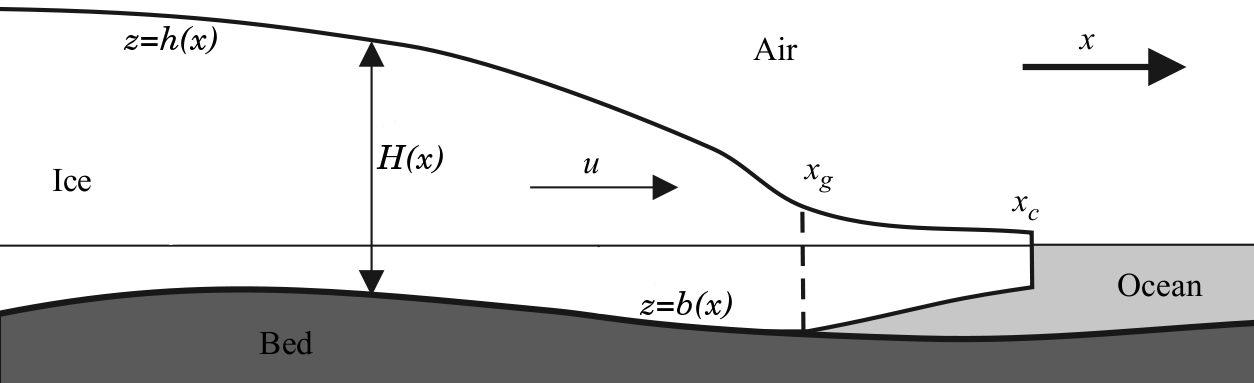
\includegraphics[width=6.0in]{flowline}
  
    \scriptsize \emph{Illustrates the notation used in these notes.  Figure modified from \cite{SchoofMarine1}.} \normalsize
    
    \vspace{1.5in}
  \end{center}
\end{titlepage}

\clearpage\newpage

%\setcounter{section}{1}
\section{Introduction}

The greatest importance of numerical models in glaciology is introspective.  You should ask yourself: When I combine my imperfect and incomplete understanding of glacier processes into this mathematical model which I put on a computer, does it behave as I expect?  Numerical models can indeed show how processes interact to give overall behavior.  They can at least demonstrate flaws in our understanding of those processes.  But they should be built with care.  An avoidable bad outcome is to spend time---or worse, reputation---interpreting, explaining, or justifying numerical model behavior that is in fact an artifact of poor computer programming or numerical analysis.

So the reader of these notes may be surprised that a continuum model, and not a computer code, seems to be our focus much of the time.  While all codes produce some numbers, we want numbers that actually come from the continuum model we have written down.  We will therefore analyse numerical implementations to see if they match the model equations and their solutions.

These notes have a limited scope:
  \begin{quote}\emph{shallow approximations of ice flow.}\end{quote}
They adopt a constructive approach; we provide:
  \begin{quote}\emph{example numerical codes that actually work.}\end{quote}
Within our scope are the shallow ice approximation (SIA) in two horizontal dimensions (2D), the shallow shelf approximation (SSA) in 1D, and the mass continuity and surface kinematical equations.  We recall the Stokes model, but we do not address its numerical solution.  Our numerical concepts include finite difference schemes, solving algebraic systems from stress balances, and the verification of codes using exact solutions.

Our notation, which generally follows \cite{GreveBlatter2009}, is common in the glaciological literature, but see Table \ref{tab:notation}.  Cartesian coordinates are $x,y,z$ with $z$ positive-upward.  If these coordinates or time $t$ appear as subscripts then they denote partial derivatives: $u_x = \partial u/\partial x$.  Tensor notation uses subscripts from the list $\{1,2,3,i,j\}$.  For example, ``$\tau_{ij}$'' or ``$\tau_{13}$'' denote entries of the deviatoric stress tensor.

These notes are based on nineteen Matlab codes, each about one-half page.  All have been tested in Matlab and Octave.  They are distributed by cloning the repository at
\begin{quote}
\url{https://github.com/bueler/mccarthy}
\end{quote}
\noindent and looking in the \texttt{mfiles/} subdirectory.  Five of these codes are printed here, with their comments stripped for compactness and clarity.  The electronic versions have generous comments and help files.

\begin{table}[ht]
\caption{Notation used in these notes, with values for some constants.}
\begin{tabular}{clll}
variable  & description & SI units & value \\
\hline
$A$ & $A=A(T)=$ ice softness in the Glen flow law & $\text{Pa}^{-n}\,\text{s}^{-1}$ \\
$B$ & ice hardness; $B=A^{-1/n}$ & $\text{Pa}\,\text{s}^{1/n}$ \\
$b$ & bedrock elevation & m \\
$c$ & specific heat in general & J kg$^{-1}$ K$^{-1}$ \\
$\nabla$ & (spatial) gradient & m$^{-1}$ \\
$\nabla\cdot$ & (spatial) divergence & m$^{-1}$ \\
$\mathbf{g}$ & gravity & m s$^{-2}$\phantom{foobar} & 9.81 \\
$H$ & ice thickness & m \\
$h$ & ice surface elevation & m \\
$\kappa$ & conductivity in general & J s$^{-1}$ m$^{-1}$ K$^{-1}$ \\
$M$ & climatic mass balance & m s$^{-1}$ \\
$n$ & exponent in Glen flow law & & 3 \\
$\nu$ & viscosity & Pa s \\
$p$ & pressure & Pa \\
$\bq$ & map-plane ice flux: $\bq = \int_{b}^{h} \bU\,dx = \bar{\bU} H$ & $\text{m}^2\,\text{s}^{-1}$ \\
$\rho$ & density of ice & kg m$^{-3}$ & 910 \\
$\rho_w$ & density of sea water & kg m$^{-3}$ & 1028 \\
$T$ & temperature & K \\
$\tau$ & norm (second invariant) of $\tau_{ij}$: $2 \tau^2 = \sum_{ij} \tau_{ij}^2$ & Pa \\
$\tau_{ij}$ & deviatoric stress tensor & Pa \\
$Du_{ij}$ & strain rate tensor & s$^{-1}$ \\
$\mathbf{U}$ & $=(u,v)$ horizontal ice velocity & m s$^{-1}$ \\
$\mathbf{u}$ & $=(u,v,w)$ 3D ice velocity & m s$^{-1}$ \\
\end{tabular}
\label{tab:notation}
\end{table}


\section{Ice flow equations}

My first goal in these notes is to get to an equation for which I can say:
\begin{center}
\emph{by numerically solving this equation, we have a usable model for an ice sheet.}
\end{center}
\noindent A ``usable'' model tends to be \emph{understood} as much as it is \emph{correct}.  Also, this first usable model will not be complete by any modern standard.  To get to my goal I first (briefly!) recall the continuum mechanical equations of ice flow.

Ice in glaciers is a moving fluid so we describe its motion by a velocity field $\mathbf{u}(t,x,y,z)$.  If the ice fluid were faster-moving than it actually is, and if it were linearly-viscous like liquid water, then it would be a ``typical'' incompressible fluid.  We would use the Navier-Stokes equations as the model:
\begin{align}
\nabla \cdot \mathbf{u} &= 0 &&\text{\emph{incompressibility}} \label{incompressible} \\
\rho \left(\mathbf{u}_t + \mathbf{u}\cdot\nabla \mathbf{u}\right) &= -\nabla p + \nabla \cdot (\nu \nabla \mathbf{u}) + \rho \mathbf{g} &&\text{\emph{stress balance}} \label{navierstokes}
\end{align}
In equation \eqref{navierstokes} the term $\mathbf{u}_t + \mathbf{u}\cdot\nabla \mathbf{u}$ is an acceleration.  The right-hand side of \eqref{navierstokes} is the total stress, and so equation \eqref{navierstokes} says ``$ma=F$'', i.e.~it is Newton's second law.  Much time has been spent to get partial understanding of the rich solutions of these Navier-Stokes equations; a book-length introduction like \cite{Acheson} is recommended.  The numerical solution of these equations is \emph{computational fluid dynamics} (CFD).

But, is ice flow modelling a part of CFD?  (And does a well-written general-purpose CFD text like \cite{Wesseling} help the glaciers student?)  It is true that ice sheet flow can be a large-scale fluid problem like atmosphere and ocean circulation in climate systems, but it is an odd one.  Consider some topics which might make ocean circulation modelling exciting, for example:
  \begin{center} turbulence \qquad convection \qquad  coriolis force  \qquad density stratification
  \end{center}
None of these topics are relevant to ice flow.  What could be interesting about the flow of slow, and surely boring, ice?

First observe that ice is indeed a slow fluid.  In terms of equation \eqref{navierstokes}, ``slow'' means $\rho \left(\mathbf{u}_t + \mathbf{u}\cdot\nabla \mathbf{u}\right) \approx 0$, which says that the forces (stresses) of inertia are negligible.  However, ice is also a shear-thinning fluid with a specific kind of nonlinearly-viscous (``non-Newtonian'') behavior in which larger shear strain rates imply smaller viscosity.  The viscosity $\nu$ in \eqref{navierstokes} is therefore not constant, and so we must separately state an empirically-based flow law in addition to restating \eqref{navierstokes} for slow flows.

\subsection*{Stokes equations}  The standard model for isothermal ice flow is this set of equations:
\begin{align}
\nabla \cdot \mathbf{u} &= 0 &&\text{\emph{incompressibility}} \label{incompressibleagain} \\
0 &= - \nabla p + \nabla \cdot \tau_{ij} + \rho \mathbf{g} &&\text{\emph{stress balance}} \label{forcebalance} \\
Du_{ij} &= A \tau^2 \tau_{ij} &&\text{\emph{$n$=3 Glen flow law}} \label{flowlaw}
\end{align}
In the flow law \eqref{flowlaw}, the deviatoric stress tensor $\tau_{ij}$ and the strain rate tensor $Du_{ij}$ appear; previous lectures cover these.  Here we merely note that: $Du_{ij} = (1/2)((u_i)_{x_j}+(u_j)_{x_i})$ if we index coordinates by $x_1,x_2,x_3=x,y,z$, each tensor in \eqref{flowlaw} is symmetric and has trace zero, and $\tau^2 = (1/2) \tau_{ij} \tau_{ij}$ (using the summation convention).

The Stokes equations do not contain a time derivative.  Thus boundary stresses, the force of gravity $\rho \mathbf{g}$, and ice softness $A$ together determine the velocity and stress fields (i.e.~$\bu$, $p$, $\tau_{ij}$) instantaneously.  Thus ice flow simulation codes have no memory of prior momentum or velocity.  Said another way, velocity is a ``diagnostic'' output of ice flow codes, because it is not needed for (re)starting a simulation.

\subsection*{Plane-flow Stokes equations}  Consider now the $x,z$-plane case of equations \eqref{incompressibleagain}, \eqref{forcebalance}, and \eqref{flowlaw}.  ``Plane-flow'' means that velocity component $v$ is zero and that all derivatives with respect to $y$ are zero:
\begin{align}
u_x + w_z &= 0 &&\text{\emph{incompressibility}} \label{incompressiblexz} \\
p_x &= \tau_{11,x} + \tau_{13,z} &&\text{\emph{stress balance} ($x$)} \label{stokespx} \\
p_z &= \tau_{13,x} - \tau_{11,z} - \rho g &&\text{\emph{stress balance} ($z$)} \label{stokespz} \\
u_x &= A \tau^2 \tau_{11} &&\text{\emph{flow law} (diagonal)}  \label{forceflowx} \\
u_z + w _x &= 2 A \tau^2 \tau_{13} &&\text{\emph{flow law} (off-diagonal)} \label{forceflowz}
\end{align}
Note that $\tau_{13}$ is a shear stress while $\tau_{11}$ and $\tau_{33}=-\tau_{11}$ are deviatoric longitudinal stresses.  Also $\tau^2 = \tau_{11}^2+\tau_{13}^2$ in this case.  Equations \eqref{incompressiblexz}--\eqref{forceflowz} form a system of five nonlinear equations in five scalar unknowns ($u,w,p,\tau_{11},\tau_{13}$).

\subsection*{Slab-on-a-slope}  Equations \eqref{incompressiblexz}--\eqref{forceflowz} are complicated enough to make us pause before jumping in to numerical solution methods, but  we can handle a simplified situation first.  A uniform slab of ice, or a ``slab-on-a-slope'', is both a case in which we can actually solve the Stokes equations, and a motivation for the shallow model in the next subsection.

\onefig{slab}{Rotated axes for a slab-on-a-slope flow calculation.}

We rotate our coordinates only for this example and not elsewhere in these notes.  The two-dimensional axes ($x$,$z$) shown in Figure \ref{fig:slab} are rotated downward (clockwise) at angle $\alpha>0$ so that the gravity vector has components $\mathbf{g} = (g \sin\alpha,- g \cos \alpha)$.  Equations \eqref{stokespx} and \eqref{stokespz} in these rotated coordinates are
\begin{align}
p_x &= \tau_{11,x} + \tau_{13,z} + \rho g \sin\alpha, \label{stokespxrot} \\
p_z &= \tau_{13,x} - \tau_{11,z} - \rho g \cos\alpha. \label{stokespzrot}
\end{align}
Assuming also that there is no variation with $x$, the whole set of Stokes equations \eqref{incompressiblexz}, \eqref{forceflowx}, \eqref{forceflowz}, \eqref{stokespxrot}, \eqref{stokespzrot} simplifies greatly:
\begin{align}
w_z &= 0 &   0 &= \tau_{11} \label{stokesslab} \\
\tau_{13,z} &= - \rho g \sin\alpha &   u_z &= 2 A \tau^2 \tau_{13} \notag \\
p_z &= -\tau_{11,z} = - \rho g \cos\alpha \notag
\end{align}
We apply boundary conditions for these functions of $z$: $w(0)=0$, $p(H)=0$, $u(0)=u_0$.  The basal velocity $u_0$ will remain undetermined for now.

By integrating equations \eqref{stokesslab} with respect to $z$, and using $\tau_{11}=0$, we get $w=0$, $p = \rho g \cos\alpha (H-z)$, and $\tau_{13} = \rho g \sin\alpha (H-z)$.  Note that $H-z$ is the depth below the ice surface, so both the pressure $p$ and shear stress $\tau_{13}$ are proportional to depth.  Because $u_z = 2 A \tau^2 \tau_{13}$, by integrating vertically again we find the horizontal velocity:
\begin{align}
u &= u_0 + \frac{1}{2} A (\rho g \sin\alpha)^3  \left(H^4 - (H-z)^4\right)  \label{uslab}
\end{align}

Do we believe formula \eqref{uslab}?  Figure \ref{fig:slabvel} compares it to observations of a mountain glacier, and it shows we have already done a credible job of capturing deformation flow velocity in this case.  We do not yet have a model for the sliding velocity $u_0$ (i.e.~basal motion).  

\twofigsizes{slabvel}{athabasca-deform}{Left:  Velocity from slab-on-a-slope formula \eqref{uslab}.  Right:  Inclinometry-measured velocity in a glacier (Athabasca Glacier \cite{SavagePaterson}).}{2.0in}{1.8in}

\subsection*{Plane-flow mass-continuity equation}  Observe that the equations so far do not address the change in shape of the glacier or ice sheet.  For this we need another equation, the \emph{mass continuity equation}.  We consider the general case of an $x,z$-plane flow with variable thickness and velocity, not just slab-on-a-slope.  Define the vertical average of the horizontal velocity:
	$$\bar U = \frac{1}{H}\int_0^{H} u\,dz.$$
The flux $q=\bar U\, H = \int_0^{H} u\,dz$ is the rate of flow input into the side of the area in Figure \ref{fig:slabmasscontfig}.

\onefigsize{slabmasscontfig}{Mass continuity equation \eqref{masscont1D} follows from considering the changing area $A$ of ice in a planar flow.  Ice can be added by surface mass balance $M$ or a difference of flux $q=\bar u H$ into the left and right sides.}{2.5in}

The ice area $A$ in Figure \ref{fig:slabmasscontfig} changes according to the sum of all the boundary contributions,
\begin{equation}
\frac{dA}{dt} = \int_{x_1}^{x_2} M(x)\,dx + \bar U_1 H_1 - \bar U_2 H_2: \label{masscontintegrated}
\end{equation}
Here $M(x)$ is the climatic mass balance at the ice surface.  (In three-dimensions, equation \eqref{masscontintegrated} would become an equation for $dV/dt$, the rate of change of ice volume.)

If the width $\Delta x=x_2-x_1$ is small then $A\approx \Delta x\, H$.  So we divide by $\Delta x$ and take $\Delta x \to 0$ in \eqref{masscontintegrated} and get
\begin{equation}
H_t = M - \left(\bar U H\right)_x \label{masscont1D}
\end{equation}
This mass continuity equation describes change in the ice thickness in terms of surface mass balance and ice velocity.  An important aspect of ice flow simulations is how one computes the velocity which goes into this equation.

\subsection*{Viscosity form of the flow law}  The flow law \eqref{flowlaw} has another form which we will use next, and also later in describing ice shelf and stream flow.  Recall $\tau^2 = (1/2) \tau_{ij} \tau_{ij}$ and also define $|Du|^2 = (1/2) Du_{ij} Du_{ij}$.  The scalars $\tau$ and $|Du|$ are norms (also ``second invariants'') of the tensors $\tau_{ij}$ and $Du_{ij}$, respectively.  By taking these norms of both sides of \eqref{flowlaw} we get $|Du| = A \tau^3$.  But then $\tau = A^{-1/3} |Du|^{1/3}$, so \eqref{flowlaw} can be rewritten
\begin{equation}
\tau_{ij} = 2 \nu\, Du_{ij}  \qquad \text{\emph{flow law (viscosity form)}} \label{viscosityflowlaw}
\end{equation}
where $\nu = (1/2) A^{-1/3} |Du|^{-2/3}$ is the nonlinear viscosity.  Often $B = A^{-1/3}$ is called the ice ``hardness''.  The derivation of \eqref{viscosityflowlaw} is worth knowing in detail; see the Exercises.

Form \eqref{viscosityflowlaw} of the flow law allows us to eliminate stresses $\tau_{ij}$ from the Stokes equations by replacing them with formulas depending on derivatives of the velocity.  That is, one can write the Stokes equations in terms of the strain rates only.  The next two approximate models also use this idea.

\subsection*{The Blatter-Pattyn approximation}  We return now briefly to plane-flow Stokes equations \eqref{incompressiblexz}--\eqref{forceflowz}, and reconsider how to simplify them.  One simplification step, present in all shallow models, is to drop the single term  $\tau_{13,x}$ from the $z$-component of the stress balance \eqref{stokespz}.  This assumes that horizontal variation in the vertical shear stress is small compared to the other terms:
\begin{equation}
p_z = - \tau_{11,z} - \rho g. \label{hydrostaticpz}
\end{equation}
Because the (Cauchy) stress tensor $\sigma_{ij}$ is related to the deviatoric stress tensor by $\sigma_{ij} = \tau_{ij} - p \delta_{ij}$, and thus $p + \tau_{11} = p - \tau_{33} = - \sigma_{33}$, equation \eqref{hydrostaticpz} says that the vertical normal stress $\sigma_{33}$ is linear in depth; this is similar to a statement that the ice is hydrostatic.  Taking it to have surface value zero we get
\begin{equation}
p + \tau_{11} = \rho g (h-z). \label{hydrostaticitself}
\end{equation}

Equation \eqref{hydrostaticitself} allows one to eliminate $p$ from the model equations.  Furthermore, taking the $x$-derivative of \eqref{hydrostaticitself} and substituting into \eqref{stokespx}, then using the viscosity form \eqref{viscosityflowlaw}, leads to this equation (Notes and References and \cite{GreveBlatter2009}):
\begin{equation}
\left(4 \nu u_x\right)_x + \left(\nu (u_z+w_x)\right)_z = \rho g h_x \qquad\text{\emph{hydrostatic stress balance}} \label{stresshydrostatic}
\end{equation}
The hydrostatic stress balance equation \eqref{stresshydrostatic} is nontrivially-coupled to incompressibility \eqref{incompressiblexz} because derivatives of the vertical velocity $w$ appear in both equations, though $p$ is gone.  Nonetheless coupled equations \eqref{incompressiblexz} and \eqref{stresshydrostatic}, along with the formula $\nu = (1/2) A^{-1/3} |Du|^{-2/3}$ and appropriate boundary conditions, determine $u$ and $w$.

If we drop $w_x$ from equation \eqref{stresshydrostatic} then we get the Blatter-Pattyn model:
\begin{equation}
\left(4 \nu u_x\right)_x + \left(\nu u_z\right)_z = \rho g h_x \qquad\text{\emph{Blatter-Pattyn stress balance}} \label{stressblatter}
\end{equation}
Using this equation one can solve first for the horizontal velocity $u$ and then afterward recover $w$ from \eqref{incompressiblexz}; stress balance and incompressibility are decoupled.

\section{Shallow ice sheets}

Ice sheets have four outstanding properties as fluids.  They are (\emph{i}) slow, (\emph{ii}) shallow,  (\emph{iii}) non-Newtonian, and (\emph{iv}) they experience some contact slip (basal sliding).  The first ice flow model which we solve numerically in these notes is the non-sliding, isothermal \emph{shallow ice approximation} (SIA).  It accounts for (\emph{i})--(\emph{iii}).

Regarding the property of shallowness, Figure \ref{fig:green-transect} shows both a no-vertical-exaggeration cross-section of Greenland at $71^\circ$, as well as the standard vertically-exaggerated version which is more familiar in the glaciological literature.  In other words, ice sheets \emph{are} shallow, though of course the portion of an ice sheet which you want to model may not be.

\onefig{green-transect}{A vertically-exaggerated cross-section of the Greenland ice sheet ($71^\circ$ N) is shown by the upper two curves.  Without exaggeration it appears as merely a thickened horizontal line.}

Our slab-on-a-slope example gives us a rough explanation of the SIA.  To show the SIA in its plane-flow form, we vertically integrate velocity formula \eqref{uslab} in the $u_0=0$ (non-sliding) case to get
\begin{equation}
\bar u H = \int_0^H \frac{1}{2} A (\rho g \sin\alpha)^3  \left(H^4 - (H-z)^4\right)\,dz = \frac{2}{5} A (\rho g \sin\alpha)^3 H^5. \label{siaubar}
\end{equation}
Note $\sin \alpha \approx \tan\alpha = - h_x$.  Combining these statements with mass continuity \eqref{masscont1D} gives
\begin{equation}
  H_t = M + \left(\frac{2}{5} (\rho g)^3 A H^5 |h_x|^2 h_x\right)_x. \label{sia1D}
\end{equation}

Equation \eqref{sia1D} is the SIA equation for nonsliding plane flow.  It is the promised first usable model for the evolution of an ice sheet's thickness $H$ in terms of surface mass balance $M$, ice softness $A$, and bed elevation $b$ (because $h=H+b$).  The model must, however, be solved subject to the constraint that the thickness is positive ($H\ge 0$); see Notes and References.

Additional arguments are needed to demonstrate that the SIA is more general-purpose than the special case of a simple slab; see Notes and References.  Such arguments reduce the Stokes equations under the assumption that the surface and bed slopes, and the depth-to-width ratio, are small.

We will numerically solve the SIA in section \ref{sec:numericalsia}, but first we state it in two horizontal dimensions.  Let $\mathbf{U} = (u,v)$ be the vector horizontal velocity.  The shear stress approximation is $(\tau_{13},\tau_{23}) \approx - \rho g (h-z) \nabla h$, which appeared as ``$\tau_{13}= \rho g \sin \alpha (h-z)$ and $\sin \alpha \approx -h_x$'' in the previous section, becomes an equality in the SIA.  Equation \eqref{flowlaw} then gives the SIA formula for shear strain rates
\begin{equation*}
\mathbf{U}_z = 2 A |(\tau_{13},\tau_{23})|^{n-1} (\tau_{13},\tau_{23}) = - 2 A (\rho g)^n (h-z)^n |\nabla h|^{n-1} \nabla h.
\end{equation*}
By integrating vertically we get, in the non-sliding case,
\begin{equation}
\mathbf{U} = - \frac{2 A (\rho g)^n}{n+1} \left[H^{n+1} - (h-z)^{n+1}\right] |\nabla h|^{n-1} \nabla h.  \label{siavelocity}
\end{equation}

Mass continuity in two horizontal dimensions, which generalizes the 1D version \eqref{masscont1D}, also applies:
\begin{equation}
    H_t = M - \Div\left(\bar{\mathbf{U}} H\right)  \label{masscont}
\end{equation}
Equation \eqref{masscont} may be written $H_t = M - \Div \bq$ in terms of the map-plane flux $\bq = \int_{b}^{h} \mathbf{U}\,dz = \bar{\mathbf{U}}\,H$.

Combining Equations \eqref{siavelocity} and \eqref{masscont}, we get an equation for the rate of thickness change in terms of mass balance $M$, thickness, and surface slope $\grad h$:
\begin{equation}
H_t = M + \Div \left(\Gamma H^{n+2} |\grad h|^{n-1} \grad h \right), \label{sia}
\end{equation}
where we have defined the positive constant $\Gamma = 2 A (\rho g)^n / (n+2)$.  Equation \eqref{sia} is the SIA in two dimensions.  Recalling our earlier promise, if we can solve \eqref{sia} numerically then we have, following Mahaffy \cite{Mahaffy}, a usable model for the Barnes ice cap in Canada, a particularly-simple ice sheet on a rather flat bed.

\subsection*{Analogy with the heat equation}  The SIA model is easy to compare with the better-known heat equation.  Numerical methods for solving \eqref{sia} can be understood as modifications of well-known heat equation methods.

In the simplest one-dimensional (1D) case, the heat equation for the temperature $T(t,x)$ of a conducting rod is
\begin{equation}
  T_t = D T_{xx}. \label{heat1D}
\end{equation}
This form applies when material properties are constant and there are no heat sources.  The positive constant $D$ is the ``diffusivity,'' with units which can be read from comparing sides of the equation: $D\sim \text{m}^2 \text{s}^{-1}$.  Observe that equation \eqref{heat1D} has a smoothing effect on the solution $T$ as it evolves in time, because any local maximum in the temperature is flattened (i.e.~$T_{xx}<0$ implies $T_t<0$ so $T$ decreases), while any local minimum is also flattened (i.e.~$T_{xx}>0$ implies $T_t>0$ so $T$ increases).

We will state the 2D heat equation more generally.  It describes the temperature $T(t,x,y)$ of some planar object, at position $x,y$ and time $t$.  Recall that Fourier's law for conduction is the formula $\mathbf{Q} = - \kappa \grad T$ for heat flux $\mathbf{Q}$, where $\kappa$ is conductivity.  We will assume, for the purposes of our analogy, that $\kappa(x,y)$ may vary in space.  Also suppose there is a variable heat source $f(t,x,y)$, with units of Watts per cubic meter.  Then conservation of internal energy says
\begin{equation}
\rho c T_t = f + \Div (\kappa \grad T). \label{heatearly}
\end{equation}
Here $\rho$ is density and $c$ is specific heat capacity.  Assuming $\rho c$ is constant, define the ``diffusivity'' $D=\kappa/(\rho c)$ and the rescaled source term $F = f/(\rho c)$.  The revised 2D heat equation is
\begin{equation}
T_t = F + \Div (D\, \grad T). \label{heat}
\end{equation}
It clearly generalizes equation \eqref{heat1D}.

Figure \ref{fig:initialheat} shows a solution of heat equation \eqref{heat}, wherein the initial condition is a localized ``hot spot''.  Solutions of the heat equation always involve the spreading, in all directions, of any local heat maxima or minima, that is, diffusion.

\twofigsizes{initialheat}{finalheat}{A solution of heat equation \eqref{heat} with $D=1$ and $F=0$.  Left: Initial condition $T(0,x,y)$.   Right: Solution $T(t,x,y)$ at $t=0.02$.}{2.8in}{2.8in}

The SIA equation \eqref{sia} and the heat equation \eqref{heat} are each diffusive, time-evolving partial differential equations (PDEs).  A side-by-side comparison is illuminating:
\begin{center}
\begin{tabular}{cc}
\vspace{1mm}
SIA:\, $H$ is ice thickness & \phantom{foo bar} heat: $T$ is temperature\phantom{foo bar}  \\
\vspace{1mm}
	$H_t = M + \Div \left({\color{red}\Gamma H^{n+2} |\grad h|^{n-1}}\, \grad h \right)$  &  $T_t = F + \Div (D\, \grad T)$
\end{tabular}
\end{center}
\vspace{1mm}
Notice that the number of derivatives (one time and two space derivatives) and the signs are the same.  Surface mass balance $M$ is analogous to heat source $F$.  

The analogy suggests that we identify the \emph{diffusivity in the SIA} as:
\begin{equation}
	D = {\color{red}\Gamma H^{n+2} |\grad h|^{n-1}}.  \label{siadiffusivity}
\end{equation}
A non-sliding SIA flow diffuses the thickness of the ice sheet, and when this $D$ comes out large then the diffusion acts most quickly.  Being a product of $\Gamma$ and the powers of $H$ and $|\grad h|$, this diffusivity $D$ is large if the ice is both thick and steep.  In summary, ice diffuses (i.e.~flows downhill) more when it is thick and steep.

This diffusion equation analogy explains generally why the surfaces of ice sheets are smooth, at least if we overlook non-flow processes like crevassing and wind-driven (snow) dunes.  There are, however, some practical and conceptual issues with the analogy:
\begin{itemize}
\item The diffusivity $D$ in \eqref{siadiffusivity} depends on the solution, both thickness $H$ and surface slope $|\grad h|$.  This affects how we reason about diffusivity.  Numerical solution processes are more difficult because nonlinear equations are harder to solve.
\item The diffusivity $D$ in \eqref{siadiffusivity} goes to zero at margins, where $H\to 0$, and at divides and domes, where $|\grad h|\to 0$.  This means that the solution is not smooth, even though the thickness is continuous everywhere (and zero outside the ice sheet).  A non-smooth solution generates larger numerical errors.
\end{itemize}
More important is a deficiency of the SIA model, and not the analogy \emph{per se}, namely
\begin{itemize}
\item Ice flow is much less diffusive when significant longitudinal (membrane) stresses are present, as when ice is floating or sliding or when the flow is confined by terrain.
\end{itemize}
Nonetheless we continue toward a verified numerical scheme for the SIA model \eqref{sia} (Section \ref{sec:numericalsia}).  The next Section introduces some numerical PDE methods in general.

\section{Finite difference numerics} 

The diffusivity analogy above suggests that numerical schemes for the heat equation are a starting point for solving the SIA equation \eqref{sia}.  Here we demonstrate only finite difference (FD) schemes, in which we replace derivatives by mere arithmetic.

The basic fact on which FD schemes are based is \emph{Taylor's theorem}, which says that for a smooth function $f(x)$,
	$$f(x+\Delta) = f(x) + f'(x) \Delta + \frac{1}{2} f''(x) \Delta^2 + \frac{1}{3!} f'''(x) \Delta^3 + \dots$$
You can replace ``$\Delta$'' by its multiples, for example:
\begin{align*}
f(x+2\Delta) &= f(x) + 2 f'(x) \Delta + 2 f''(x) \Delta^2 + \frac{4}{3} f'''(x) \Delta^3 + \dots \\
f(x-\Delta) &= f(x) - f'(x) \Delta + \frac{1}{2} f''(x) \Delta^2 - \frac{1}{3!} f'''(x) \Delta^3 + \dots
\end{align*}
The idea for constructing FD schemes is to combine expressions like these to give approximations of derivatives.  Thereby an equation relating values on a grid serves to approximate the differential equation.

Here we want partial derivative approximations, so we apply the Taylor's expansions one variable at a time.  For example, with a general function $u=u(t,x)$,
\begin{align*}
u_t(t,x) &= \frac{u(t+\Delta t,x) - u(t,x)}{\Delta t} + O(\Delta t), \\
u_t(t,x) &= \frac{u(t+\Delta t,x) - u(t-\Delta t,x)}{2\Delta t} + O((\Delta t)^2), \\
u_x(t,x) &= \frac{u(t,x+\Delta x) - u(t,x-\Delta x)}{2\Delta x} + O((\Delta x)^2), \\
u_{xx}(t,x) &= \frac{u(t,x+\Delta x) - 2\, u(t,x) + u(t,x-\Delta x)}{\Delta x^2} + O((\Delta x)^2)
\end{align*}
Note that if $\Delta$ is a small number then ``$+O(\Delta^2)$'' is smaller than ``$+O(\Delta)$'', so the approximation is closer when you drop it.

\subsection*{Explicit scheme for the heat equation}  We first build the simplest ``explicit'' scheme which approximates the 1D heat equation \eqref{heat1D}.  It is based on the fact that because $T_t$ and $D T_{xx}$ are equal, these two FD expressions are nearly equal:
\begin{equation}
\frac{T(t+\Delta t,x) - T(t,x)}{\Delta t} \approx D\,\frac{T(t,x+\Delta x) - 2\, T(t,x) + T(t,x-\Delta x)}{\Delta x^2}.  \label{heat1Dapproximated}
\end{equation}
The scheme itself is a method for computing numbers on a grid.  That is, \eqref{heat1Dapproximated} approximates the PDE, but making it into an equality tells how to \emph{determine} grid values.

Let $(t_n,x_j)$ denote the points of the time-space grid shown in Figure \ref{fig:timespacegrid}.  Denote our approximation of the solution value $T(t_n,x_j)$ by $T_j^n$.  Then the finite difference scheme is
	$$\frac{T_j^{n+1} - T_j^n}{\Delta t} = D\,\frac{T_{j+1}^n - 2\, T_j^n + T_{j-1}^n}{\Delta x^2}.$$
To get a computable formula, let $\mu = D \Delta t / (\Delta x)^2$ and solve for $T_j^{n+1}$:
\begin{equation}
  T_j^{n+1} = \mu T_{j+1}^n + (1 - 2 \mu) T_j^n + \mu T_{j-1}^n \label{heat1Dfd}
\end{equation}

\onefigsize{timespacegrid}{A grid for a finite difference solution to \eqref{heat1D}.}{2.0in}

FD scheme \eqref{heat1Dfd} is \emph{explicit} because it directly computes $T_j^{n+1}$ in terms of values at time $t_n$.  Figure \ref{fig:expstencil} (left) shows the ``stencil'' for scheme \eqref{heat1Dfd}: three values at the current time $t_n$ are combined to update the one value at the next time $t_{n+1}$.

Before moving on, notice that evaluating a heat equation solution at a grid point (i.e.~the expression ``$T(t_n,x_j)$'') is generally a different number from the value $T_j^n$ computed by a scheme like \eqref{heat1Dfd}.  We intend that the numbers $T(t_n,x_j)$ and $T_j^n$ become closer together as the grid is made finer (i.e.~$\Delta t \to 0$ and $\Delta x \to 0$), because the FD expressions become closer to the derivatives they approximate.  That is, we intend our FD scheme to \emph{converge} under \emph{grid refinement}.  For now we \emph{plan} and \emph{hope} that convergence happens, but it needs checking (``verification''; Section \ref{sec:exactsolutions}) or perhaps a proof.

\twofigsizes{expstencil}{exp2dstencil}{Left: Space-time stencil for the explicit scheme \eqref{heat1Dfd} for the 1D heat equation.  Right: Spatial-only stencil for scheme \eqref{heat2dexplicit}.}{2.0in}{2.1in}

How accurate is scheme \eqref{heat1Dfd}?  Its construction tells us that the difference between the scheme \eqref{heat1Dfd} and the PDE \eqref{heat1D} is $O(\Delta t + (\Delta x)^2)$, so this difference goes to zero as we refine the grid in space and time, a property called \emph{consistency}.  With care about the smoothness of boundary conditions, and using mathematical facts about the heat equation itself, one can show that the difference between $T_j^n$ and $T(t_n,x_j)$ is also $O(\Delta t + (\Delta x)^2)$, which is thus the \emph{convergence rate}; see Notes and References.

To get convergence the PDE problem must generate adequately smooth solutions, and also scheme \eqref{heat1Dfd} must be \emph{stable}, which we address below.  The main theorem for numerical PDE schemes is ``consistency plus stability implies convergence''; see Notes and References.  Instead of pursuing such theory, however, these notes we do something rather practical, namely verification.  We find problems for which we already know an exact solution $T(t,x)$, and then we compute the differences $|T_j^n - T(t_n,x_j)|$.  This determines directly whether our actual \emph{implementation} (i.e.~computer code form of the scheme) actually does converge, not just whether it should in theory.

\subsection*{A first implemented scheme}  Our first Matlab implementation is for the 2D Equation \eqref{heat} with $D$ constant and $F=0$:
\begin{equation}
T_t = D (T_{xx}+T_{yy}).\label{heat2D}
\end{equation}
Writing $T_{jk}^n \approx T(t_n,x_j,y_k)$, the 2D explicit scheme is
\begin{equation}
	\frac{T_{jk}^{n+1} - T_{jk}^n}{\Delta t} = D\,\left(\frac{T_{j+1,k}^n - 2\, T_{jk}^n + T_{j-1,k}^n}{\Delta x^2} + \frac{T_{j,k+1}^n - 2\, T_{jk}^n + T_{j,k-1}^n}{\Delta y^2}\right). \label{heat2dexplicit}
\end{equation}
The stencil for the right-hand side of \eqref{heat2dexplicit} is shown in Figure \ref{fig:expstencil} (right).

Scheme \eqref{heat2dexplicit} has implementation \texttt{heat.m} below.  For simplicity we set $T=0$ on the boundary of the square $-1 < x < 1$, $-1 < y < 1$.  The initial condition is gaussian: $T(0,x,y) = \exp(-30 (x^2+y^2))$.  The code uses Matlab ``colon'' notation to remove loops over spatial variables.  Here is an example run:
\begin{Verbatim}
>>  heat(1.0,30,30,0.001,20);
\end{Verbatim}
This sets $D=1.0$ and uses a $30\times 30$ spatial grid.  We take $N=20$ time steps of $\Delta t = 0.001$.  The result is shown in Figure \ref{fig:initialheat}, right.  This is the look of success.

\minput{heat}

However, very similar runs seem to succeed or fail according to some as-yet unclear circumstances.  For example, results from these calls are shown in Figure \ref{fig:stability}:
\begin{Verbatim}
>> heat(1.0,40,40,0.0005,100);    % Figure 8, left
>> heat(1.0,40,40,0.001,50);      % Figure 8, right
\end{Verbatim}
Both runs compute temperature $T$ on the same spatial grid, for the same final time $t_f = N \Delta t = 0.05$, but with different time steps.  Noting the vertical axes, the second run clearly shows ``instability,'' an extreme form of inaccuracy characterized in practice by numbers of a totally different magnitude than expected.

\twofig{stability}{instability}{Numerically-computed temperature on $40\times 40$ grids.  The two runs are the same except that the left has $\Delta t=0.0005$ so $D\Delta t/(\Delta x)^2= 0.2$, while the right has $\Delta t=0.001$ so $D\Delta t/(\Delta x)^2= 0.4$.  Compare \eqref{stabcrit}.}


\subsection*{Stability criteria and adaptive time stepping}  To avoid the instability shown at right in Figure \ref{fig:stability}, we need to understand the scheme better.  It turns out we have not made an implementation error.  Instead, care is required when choosing space and time steps.

Recall the 1D explicit scheme in form \eqref{heat1Dfd}: $T_j^{n+1} = \mu T_{j+1}^n + (1 - 2 \mu) T_j^n + \mu T_{j-1}^n$.  The new value $T_j^{n+1}$ is an average of the old values, in the sense that the coefficients add to one.  Averaging is stable because averaged wiggles are smaller than the wiggles themselves.  Actually, however, the scheme is only an average \emph{if} the middle coefficient is positive, as a linear combination with coefficients which add to one is not an average if any coefficients are negative.  (For example, one would not accept 15 as an ``average'' of 5 and 7, but: $15 = -4 \times 5 + 5 \times 7$, and $-4+5=1$.)

So, what follows from requiring the middle coefficient in \eqref{heat1Dfd} to be positive so it computes such an average?  A \emph{stability criterion} follows, with these equivalent forms:
\begin{equation}
   1 - 2 \mu \ge 0 \quad \iff \quad \frac{D\Delta t}{\Delta x^2} \le \frac{1}{2} \quad \iff \quad \Delta t \le \frac{\Delta x^2}{2 D}.  \label{stabcrit}
\end{equation}
The third form states the condition as a limitation on the size of $\Delta t$.  It is a \emph{sufficient} stability criterion; it is enough to guarantee stability, though something weaker might do.  In summary, for given $\Delta x$, shortening the time steps $\Delta t$ so that \eqref{stabcrit} holds will make FD scheme \eqref{heat1Dfd} into an averaging process.

Applying this same idea to the 2D heat equation \eqref{heat2D} leads to the stability condition that $1-2\mu^x-2\mu^y \ge 0$ where $\mu^x = D \Delta t / (\Delta x^2)$ and $\mu^y = D \Delta t / (\Delta y^2)$.  In the cases shown in Figure \ref{fig:stability}, wherein $\Delta x=\Delta y$, this condition requires $D \Delta t /(\Delta x^2) \le 0.25$.  This inequality precisely distinguishes between the two parts of Figure \ref{fig:stability}.

In summary, runs of \texttt{heat.m} are unstable if the time step $\Delta t$ is too big relative to the spacing $\Delta x$.  The stability criterion is, however, satisfied by making each time step shorter.  Enforcing the criterion inside the code itself is an \emph{adaptive} implementation.  Such an implementation can be stable even if the diffusivity $D$ is changing in time.  To show how easy this is to implement, \texttt{heatadapt.m} (not shown) is the same as \texttt{heat.m} except that the time step comes from the stability criterion.  However, if the diffusivity $D$ is large or the grid spacings $\Delta x$, $\Delta y$ are small, then adaptive explicit implementations must take many short time steps to assure stability.  Adaptive explicit schemes can be slow.


\subsection*{Implicit schemes}  There is an alternative stability fix instead of adaptivity, namely ``implicitness.''  For example, the finite difference scheme
\begin{equation}
  \frac{T_j^{n+1} - T_j^n}{\Delta t} = D\,\frac{T_{j+1}^{n+1} - 2\, T_j^{n+1} + T_{j-1}^{n+1}}{\Delta x^2} \label{implicit1D}
\end{equation}
is an $O(\Delta t + (\Delta x)^2)$ implicit scheme for Equation \eqref{heat1D}.  This implicit scheme for the heat equation is stable for \emph{any} positive time step $\Delta t>0$ (``unconditionally stable''); see Notes and References.  Another well-known implicit scheme is \emph{Crank-Nicolson}, which is unconditionally stable for the heat equation, but with smaller error $O((\Delta t)^2 +(\Delta x)^2)$.

Implicit schemes are harder to implement because the unknown solution values at time step $t_{n+1}$ are treated as a vector in a large system of equations which must be formed and solved at each time step.  If the PDE is nonlinear then the system of equations may be hard to solve.  Though the SIA is a highly nonlinear diffusion equation, implicit schemes are becoming useful \cite{Bueler2016}.  Because of the tradeoff between the easy implementability of adaptive explicit schemes and the better stability of implicit schemes, for these notes we stay with adaptive explicit (FD) schemes.

\subsection*{Numerical solution of diffusion equations}  We are trying to numerically model ice flows, not heat conduction.  We have an analogy, however, which says that the SIA is diffusive like the heat equation.  In this section, because we wish to solve the SIA on real bedrock, we construct a numerical scheme for a more general diffusion equation which has an extra ``shift'' inside the gradient, namely
\begin{equation}
  T_t = F + \Div \left(D \grad (T + b)\right). \label{gendiffusion}
\end{equation}
In equation \eqref{gendiffusion}, the source term $F(x,y)$, the diffusivity $D(x,y)$, and the ``shift'' $b(x,y)$ may all vary in space.

The following code solves \eqref{gendiffusion}.  It is called by the SIA-specific schemes we build next.

\minput{diffusion}

This adaptive explicit method for the diffusion equation is conditionally stable, with the same essential time step restriction as for the constant diffusivity case, as long as we evaluate $D(x,y)$ at \emph{staggered} grid points.  That is, we use this expression for the second derivative:
\begin{align*}
\Div \left(D \grad X\right) &\approx \frac{D_{j+1/2,k}(X_{j+1,k} - X_{j,k}) - D_{j-1/2,k}(X_{j,k} - X_{j-1,k})}{\Delta x^2} \\
	&\qquad + \frac{D_{j,k+1/2}(X_{j,k+1} - X_{j,k}) - D_{j,k-1/2}(X_{j,k} - X_{j,k-1})}{\Delta y^2},
\end{align*}
where $X=T+b$.  The left part of Figure \ref{fig:diffstencil} shows the stencil.

\twofigsizes{diffstencil}{mahaffystencil}{Left:  Spatial stencil for staggered grid evaluation of diffusivity (at triangles) in the diffusion equation \eqref{gendiffusion}.  Right: Stencil showing how the staggered-grid diffusivity (triangle) can be evaluated in the SIA, from surface elevation (diamonds) and thicknesses (squares).}{2.2in}{2.2in}

The user supplies the diffusivity $D(x,y)$ to \texttt{diffusion.m} on the staggered grid.  The initial temperature $T(0,x,y)$, source term $F(x,y)$, and ``shift'' $b(x,y)$ are also supplied on the regular grid.  When using this code for standard diffusions, or for the flat-bed case of the SIA, we would take $b=0$.


\section{Numerically solving the SIA} \label{sec:numericalsia}

In SIA equation \eqref{sia} we have diffusivity $D = \Gamma H^{n+2} |\grad h|^{n-1}$.  As already noted, an interesting aspects of this formula is that $D$ goes to zero, the diffusion ``degenerates,'' when either $H\to 0$ or $\grad h \to 0$.  Degenerate diffusion equations are automatically free boundary problems, but this aspect of the thickness evolution problem should be no surprise to a glaciologist.  Determining the location of the margin is an obvious part of modelling a glacier or ice sheet.  To address this free boundary issue in our explicit time-stepping code it suffices to numerically compute new thicknesses and then set them to zero if they come out negative.

Second, for numerical stability and mass conservation we should compute $D$ on a ``staggered'' grid.  Various finite difference schemes for computing it have been proposed.  All of these schemes involve averaging $H$ and differencing $h$ in a ``balanced'' way onto the staggered grid.  In the code \texttt{siaflat.m} below we use the Mahaffy \cite{Mahaffy} method, with the stencil for computing $D$ shown in Figure \ref{fig:diffstencil} (right).  This code only works for the flat bed, zero surface mass balance case, but we will correct these deficiencies later.

\minput{siaflat}


\section{Exact solutions and verification} \label{sec:exactsolutions}

In \texttt{siaflat.m}, which calls \texttt{diffusion.m}, we already have a fairly complicated code.  How do we make sure that such an implemented numerical scheme is correct?  Here are three proposed techniques:
\begin{enumerate}
  \item don't make any mistakes, or
  \item compare your numerical results with results from other researchers, and hope that the outliers are in error, or
  \item compare your numerical results to an exact solution.   \end{enumerate}
The first two of these, which one might call ``infallibility'' and ``intercomparison,'' respectively, should be less common approaches than they are.  The last one of these, preferred to the first two by the CFD community generally \cite{Wesseling}, is called ``verification.''

It is a simple idea:  When we build a new computer code we should test it in cases where we know the right answer.  To do so we need to return to the PDE itself, to get useful exact solutions.

\subsection*{Exact solution of heat equation}  First we return to the simpler case of the 1D heat equation with constant $D$, namely $T_t = D T_{xx}$.  Many exact solutions $T(t,x)$ to this heat equation are known, but let's consider the time-dependent ``Green's function,'' also known as the ``heat kernel''.  It starts at time $t=0$ with a delta function $T(0,x)=\delta(x)$ of heat at the origin $x=0$.  Then it spreads out over time.  It is a solution of the heat equation on the whole line $-\infty<x<\infty$ and for all $t>0$.

We will calculate this exact solution by a method which generalizes to the SIA.  In both cases the Green's function is ``self-similar'' over time, in the sense that it changes shape \emph{only} by shrinking the output (vertical) axis and lengthening the input (horizontal) axis, as shown in Figure \ref{fig:heatscaling} for the heat equation.  These scalings are related to each other by conservation of energy, which says that the total heat energy is independent of time.

\onefigsize{heatscaling}{The heat equation Green's function in 1D has the same shape at each time, but with time-dependent input- and output-scalings.}{2.4in}

The Green's function of the 1D heat equation is
  $$T(t,x) = (4 \pi D t)^{-1/2}\, e^{-x^2/(4Dt)}.$$
``Similarity'' variables for this solution, the above-mentioned scalings, involving multiplying the input and output of an invariant shape function $\phi(s) = (4 \pi D)^{-1/2}\, e^{-s^2/(4D)}$ by the same power of $t$:
\begin{equation}
s \stackrel{\text{\emph{input scaling}}}{\phantom{\Big|}=\phantom{\Big|}} t^{-1/2} x, \qquad\qquad T(t,x) \stackrel{\text{\emph{output scaling}}}{\phantom{\Big|}=\phantom{\Big|}} t^{-1/2} \phi(s).  \label{heatscalings}
\end{equation}

A numerical solver for the 1D heat equation which starts with initial values $T(t_0,x)$ taken from this exact solution should, at a later time $t$, produce numbers which are close to the exact solution $T(t,x)$; see the Exercises.

\subsection*{Halfar's similarity solution to the SIA}  Now we jump from Green's idea in about 1830 to the year 1981.  That is when P.~Halfar published the similarity solution of the SIA in the case of flat bed and zero surface mass balance.  Halfar's solution to the 2D SIA model \eqref{sia}, using a Glen exponent $n=3$, has scalings similar to \eqref{heatscalings} above:
\begin{equation}
s = t^{-1/18} r, \qquad \qquad H(t,r)=t^{-1/9} \phi(s). \label{halfarscalings}
\end{equation}
Here $r=(x^2+y^2)^{1/2}$ is the distance from the origin.  These scalings are related to each other by conservation of mass, because no mass is gained or lost through the surface. Scalings \eqref{halfarscalings} imply that, quite differently from heat, the diffusion of ice slows down severely as the shape flattens out.  Said directly, the powers $t^{-1/9}$ and $t^{-1/18}$ change very slowly for large times $t$.

\onefigsize{siascaling}{Radial sections of Halfar's solution \eqref{halfar} of the SIA equation \eqref{sia} on a flat bed with zero mass balance.  The solution is shown on $H$ (m) versus $r$ (km) axes for times $t=1,10,100,1000,10000$ years.}{5.5in}

The formula for the Halfar solution to the SIA is remarkably simple given all that it accomplishes:
\begin{equation}
H(t,r) = H_0 \left(\frac{t_0}{t}\right)^{1/9} \left[1 - \left(\left(\frac{t_0}{t}\right)^{1/18} \frac{r}{R_0}\right)^{4/3}\right]^{3/7}. \label{halfar}
\end{equation}
Here the ``characteristic time'' $t_0 = (18 \Gamma)^{-1} (7/4)^3 R_0^4 H_0^{-7}$ is a parameter which can be determined by choosing center height $H_0$ and radius $R_0$.

Formula \eqref{halfar} is plotted in Figure \ref{fig:siascaling}.  We see that for times significantly greater than $t_0$ (i.e.~$t/t_0 \gg 1$) the solution changes very slowly.  For example, the change between years $1$ and $100$ is larger than that between years $1000$ and $10000$.  The \emph{volume} of ice is, however, constant with $t$; see the Exercises.

\subsection*{Using Halfar's solution}  Formula \eqref{halfar} is simple enough to use for verifying time-dependent SIA models.  The code \texttt{verifysia.m} (not shown) takes as input the number of grid points in each ($x,y$) direction.  It uses the Halfar solution at 200 a as the initial condition, does a numerical run of \texttt{siaflat.m} above to a final time 20000 a, and then compares to the Halfar formula for that time.  By ``compares'' we mean it computes the thickness \emph{numerical error}, the absolute values of the differences between the numerical and exact thickness solutions at the final time:
\small
\begin{verbatim}
>> verifysia(20)
average thickness error     = 22.310
>> verifysia(40)
average thickness error     = 9.490
>> verifysia(80)
average thickness error     = 2.800
>> verifysia(160)
average thickness error     = 1.059
\end{verbatim}
\normalsize
We see that the average thickness error decreases with increasing grid resolution.  This is as expected for a correctly-implemented code.  What is less obvious, perhaps, is that almost any numerical implementation mistake---almost any bug---will break this property, and these errors will not shrink.

You might ask, is the Halfar solution ever useful for modelling real ice masses?  The answer is yes.  In fact, J.~Nye and others (2000; \cite{NyeIcarus2000}) compared the long-time consequences of different flow laws for the south polar cap on Mars.  In particular, they evaluated $\text{CO}_2$ ice and $\text{H}_2\text{O}$ ice softness parameters by comparing the long-time behavior of the corresponding Halfar solutions to the observed polar cap properties.  Their conclusions:
  \begin{quote}
  \dots none of the three possible [$\text{CO}_2$] flow laws will allow a 3000-m cap, the thickness suggested by stereogrammetry, to survive for $10^7$ years, indicating that the south polar ice cap is probably not composed of pure $\text{CO}_2$ ice [but rather] water ice, with an unknown admixture of dust.
  \end{quote}
This theoretical result has since been confirmed by the observation and sampling of the polar geology of Mars.

Are exact solutions like Halfar's always available when needed?  The answer is ``no'', of course, though many ice flow models do have exact solutions which are relevant to verification; see the Notes and References.  For example, we will use van der Veen's solution for ice shelves in a later section.  On the other hand, the absence of exact solutions may show that not enough thought has gone into the continuum model itself.

\subsection*{A test of robustness}  Verification is an ideal way to start testing a code.  Another kind of test is for ``robustness'' over unusual or difficult input cases.  One asks: Does the model break?  In a robustness test one does not have precise knowledge of what the code \emph{should} do, but it is a useful test if we can at least identify obviously-unreasonable outputs.

The robustness test in the program \texttt{roughice.m} (not shown) demonstrates that \texttt{siaflat.m} can handle an ice sheet with extraordinarily large ``driving stresses.''  Recall that glaciological driving stress is $\tau_d = - \rho g H \grad h$.  This quantity appears in the slab-on-a-slope example, and thus in the SIA model, as the value of the shear stress $(\tau_{13},\tau_{23})$ at the base of the ice.  The driving stress is, obviously, large when the ice is both thick and has steep surface slope $|\nabla h|$.

\twofigsizes{roughinitial}{roughfinal}{The SIA model evolves the huge-driving-stress initial ice sheet at left to the ice cap at right in only 50 model years.}{2.9in}{2.9in}

In \texttt{roughice.m} we give \texttt{siaflat.m} a randomly-generated initial ice sheet which is of the worst possible sort because it is thick (average of 3000 m) \emph{and} it has large surface slopes.  The product $H|\grad h|$ is therefore large everywhere.  The initial shape is shown in the left side of Figure \ref{fig:roughinitial}.  During the run of 50 model years on a 17 km grid, the time step is determined adaptively from \eqref{stabcrit}.  The maximum diffusivity $D$ decreases over the course of the run, as the surface becomes smooth through flow, and thus the time-step increases from about 0.0002 years to 0.2 years.  The maximum value of the driving stress decreases from $57$ bar ($= 5.7\times 10^6$ Pa) to $3.6$ bar.  At the end of the run the ice cap has the shape shown at right in Figure \ref{fig:roughinitial}.

The shape at right in Figure \ref{fig:roughinitial} is rather close to a Halfar solution \eqref{halfar}.  Halfar essentially proved that \emph{all} solutions of the zero-mass-balance SIA on a flat bed asymptotically approach \eqref{halfar}; the Halfar solution is generic and attracting.


\section{Application to the Antarctic ice sheet}

Finally we apply the model to the Antarctic ice sheet.  To do this we must first modify \texttt{siaflat.m} to allow non-flat bedrock elevation $b(x,y)$ and arbitrary surface mass balance $M(x,y)$, and we enforce non-negative thickness at each timestep.  (In other words, we must complete the mass-continuity part of the model, whereas we have already tested the flow part.)  Also we add a minimal model of interaction with the ocean, namely we calve-off any ice that satisfies the flotation.  The result is \texttt{siageneral.m} (not shown), a code only ten lines longer than \texttt{siaflat.m}.

\twofigsizes{antinitial}{antfinal}{Left: Initial surface elevation (m) of Antarctic ice sheet.  Right: Final surface elevation at end of 40 ka model run on 50 km grid.}{2.55in}{3.2in}

We use measured accumulation, bedrock elevation, and surface elevation from ALBMAPv1 data \cite{LeBrocqetal2010}.  Melt is not modelled so the climatic mass balance is equal to the precipitation rate, clearly a more-suitable approximation for Antarctica than for Greenland, for example, but still a rough approximation.  These input data are read from a NetCDF file and preprocessed by an additional code \texttt{buildant.m} (not shown).

\onefig{antvolcompare}{Ice volume of the modeled Antarctic ice sheet, in units of $10^6 \, \text{km}^3$, from runs on 50 km (red), 25 km (green), and 20 km (blue) grids.}

The code \texttt{ant.m} (not shown) calls \texttt{siageneral.m} to do the simulation in blocks of 500 model years.  The volume is computed at the end of each block.  Figure \ref{fig:antinitial} shows the initial and final surface elevations from a run of 40,000 model years on a $\Delta x = \Delta y = 50$ km grid.  The runtime on a typical laptop is a few minutes.

Areas of the Antarctic ice sheet with low-slope and (actual) fast-flowing ice experience thickening in the model, while near-divide ice in East Antarctica, in particular, thins.  Assuming the present-day Antarctic ice sheet is somewhere near steady state, we can see that these thickness differences reflect model inadequacies.  The lack of a sliding mechanism explains the thickening in low-slope areas.  The lack of thermomechanical coupling, or equivalently the constancy of ice softness, and the fact that our isothermal $A$ value is quite ``soft'', explains the thinning near the divide; see Notes and References on modelling techniques which address these inadequacies.

We should be modelling floating ice too, but the SIA is completely inappropriate to that purpose.  Floating ice is addressed in section \ref{sec:shelvesandstreams}

Figure \ref{fig:antvolcompare} compares the ice volume time series for 50 km, 25 km, and 20 km grids.  This result, namely grid dependence of the ice volume, is typical.  One cause is that most steep gradients near the ice margin are poorly resolved, but to differing degrees at these coarse resolutions.  Figure \ref{fig:antvolcompare} is a warning about the interpretation of model runs:  Even if the data is available only on a fixed grid, the model should be run at different resolutions to evaluate the robustness of the model results.


\section{Mass continuity and kinematical equations}

Recall that in the SIA the stress balance becomes formula \eqref{siavelocity} for the velocity, which combines with the mass continuity equation \eqref{masscont} to give model \eqref{sia} for evolution of the ice sheet thickness.  The SIA equation \eqref{sia} therefore combines two concepts which we will now think about separately, and in greater generality, in the remainder of these notes.

The most basic shallow assumption made by most ice flow theories\footnote{There are several inequivalent shallow theories: SIA, SSA, hybrids, Blatter-Pattyn, \dots} is that the surface and base of the ice are differentiable functions $z=h(t,x,y)$ and $z=b(t,x,y)$.  Thus surface overhang is not allowed.  Though the Stokes theory allows the fluid boundary to be a closed surface in three-dimensional space, ice sheet and glacier models take a map-plane perspective and have a well-defined ice thickness: $H=h-b$.

To pursue such ideas a bit further, let us state the ``kinematical equations'' which apply at upper and lower surfaces of the ice sheet.  Let $a$ be the (upper surface) climatic mass balance function ($a>0$ is accumulation) and $s$ be the basal melt rate function ($s>0$ is basal melting).  In the equations which follow these are measured in thickness-per-time units, but they could be in mass-per-area-per-time units also.  The net map-plane mass balance $M=a-s$, which appears in the mass continuity equation \eqref{masscont}, is the difference of these surface fluxes.

The \emph{(upper) surface kinematical equation} is 
\begin{equation}
h_t = a - \mathbf{U}\big|_h \cdot \grad h + w\big|_h,  \label{surfkine}
\end{equation}
and the \emph{base kinematical equation} is
\begin{equation}
b_t = s - \mathbf{U}\big|_b \cdot \grad b + w\big|_b.  \label{basekine}
\end{equation}
wherein $\mathbf{U}$ is the horizontal ice velocity and $w$ the vertical ice velocity.  Equations \eqref{surfkine} and \eqref{basekine} describe the movement of the ice's upper surface and lower surfaces, respectively, from the velocity of the ice and the mass balance functions at the respective surfaces.

We can now state an important mathematical fact which follows from the assumption of well-defined upper and basal surface elevations and from incompressibility.  Namely, that the surface kinematical and mass continuity equations are closely-related.  More precisely, any pair of these equations implies the third:
  \begin{itemize}
  \item the surface kinematical equation \eqref{surfkine},
  \item the base kinematical equation \eqref{basekine}, and
  \item the map-plane mass continuity equation \eqref{masscont}.
  \end{itemize}
One proves these facts by using equation \eqref{incompressible} and the Leibniz rule for differentiating integrals.  The details are left for exercises.

The bedrock is often regarded as fixed (i.e.~$b_t=0$).  In the important (and idealized) case of non-deformable bedrock and no sliding, \eqref{basekine} says that the basal value of the vertical velocity equals the basal melt rate: $w\big|_b=-s$.

\subsection*{Prognostic models}  We can now sketch the structure of a general, explicit, ``prognostic,'' i.e.~ice geometry evolving, isothermal ice sheet model.  Each time step follows this recipe:
  \begin{itemize}
  \item numerically solve a stress balance, which gives velocity $\mathbf{u}=(u,v,w)$,
    \begin{itemize}
    \item[$\circ$] the geometry of the ice mass and the stress boundary conditions determine $\mathbf{u}$
    \item[$\circ$] if the stress balance only gives $\mathbf{U}=(u,v)$, get $w$ from incompressibility \eqref{incompressible},
    \end{itemize}
  \item decide on a time step $\Delta t$ for \eqref{masscont} based on velocities and/or diffusivities,
  \item from the horizontal velocity $\mathbf{U}=(u,v)$, compute the flux $\bq = \bar{\bU} H$,
  \item update mass balance $M=a-s$ and do a time-step of \eqref{masscont} to get $H_t$,
  \item update the upper surface elevation and thickness (e.g.~$h \mapsto h + H_t \Delta t$), and repeat.
  \end{itemize}
Like most ice sheet models, we use the mass continuity equation \eqref{masscont} to describe changes in ice sheet geometry, but we could use the surface kinematical equation \eqref{surfkine} instead.

The above ``standard'' ice sheet model has many variations.  Some glaciological questions are answered just by solving the stress balance for the velocity.  Sometimes the goal is the steady state configuration of the glacier.  This may be computed more quickly than via physical time-stepping physical evolution equations to steady state, but the thickness-positive constraint then, necessarily, becomes a focus of the analysis \cite{Bueler2016,JouvetBueler2012}.  Other processes are usually simulated at each time step, such as the conservation of energy within the ice, or subglacial and supraglacial processes.  Understanding the diverse time scales associated to these processes is always an important step in designing a model which is more complete than the isothermal SIA.

When using the SIA equation \eqref{sia}, one can apparently bypass the computation of the velocity.  That is because the mass continuity equation can be written as a diffusion, with $\bq=-D\nabla h$ for the flux, instead of with the more general formula $\bq = \bar{\bU} H$.  Fast flow in ice sheets is associated with sliding and floating ice, however, and for these flows the ice geometry evolution is not a diffusion.  While the formula $\bq = \bar{\bU} H$ applies, both for the SIA and fast flow, an ice flow model is also not hyperbolic.  Fundamentally, that is because the velocity is related to the local surface gradient.  In any case, solving the stress balance for the velocity field is generally a nontrivial and obligatory step in a numerical ice flow model.  We get started on one such case in the next Section.


\section{Shelves and streams} \label{sec:shelvesandstreams}

As its name suggests, the shallow shelf approximation (SSA) stress balance applies to ice shelves.  The SSA also applies reasonably well to ice streams which have not-too-steep bed topography and low basal resistance, like those in Figure \ref{fig:siple}.

\twofigsizes{siple}{streamisbrae}{Left:  The SSA model applies to ice streams like these on the Siple Coast in Antarctica.  Color shows radar-derived surface speed.  Right: Cross sections, \emph{without} vertical exaggeration, of (\textbf{a}) the Jakobshavns Isbrae outlet glacier in Greenland and (\textbf{b}) the Whillans Ice Stream on the Siple Coast \cite{TrufferEchelmeyer}.}{2.8in}{2.9in}

But what is, and is not, an ice stream?  Ice streams slide at $50$ to $1000 \,\text{m}\,\text{a}^{-1}$, they have a concentration of vertical shear in a thin layer near base, and typically they flow into ice shelves.  Pressurized liquid water at their beds plays a critical role enabling their fast flow.  There are other fast-flowing grounded parts of ice sheets, however, called ``outlet glaciers''.  They can have even faster surface speed (up to $10 \,\text{km}\,\text{a}^{-1}$), but it is typically uncertain how much of this speed is from sliding at the base.  In an outlet glacier there is substantial vertical shear ``up'' in the ice column, sometimes caused by soft temperate ice in a significant fraction of the thickness.  Furthermore, outlet glaciers are strongly controlled by fjord-like, large-slope bedrock topography.  Figure \ref{fig:siple} (right) compares the shallowness and bedrock topography of an outlet glacier and an ice stream.  Few simplifying assumptions are appropriate for outlet glaciers, and the SSA may not be a sufficient model.

\subsection*{The shallow shelf approximation (SSA)}  We state this stress balance equation only in the plane flow (``flow-line'') and isothermal case:
\begin{equation}
  \left(2 B H |u_x|^{1/n - 1} u_x\right)_x - C|u|^{m-1}u = \rho g H h_x \label{ssaearly}
\end{equation}
The term in parentheses is the vertically-integrated longitudinal stress.  (It is called the ``membrane'' stress when there are two horizontal dimensions.)  The second term $\tau_b = - C|u|^{m-1}u$ is the basal resistance, which is zero (i.e.~$C=0$) in an ice shelf.  The term on the right is the negative of the driving stress ($\tau_d = - \rho g H h_x$).  Thus the longitudinal strain rates are determined by the integrated ice hardness (i.e.~the coefficient $BH$), the slipperyness of the bed (i.e.~by the coefficient $C$ and the power $m$) and the geometry of the ice sheet (i.e.~the thickness $H$ and the surface slope $h_x$).  The power-law formula for the basal resistance $\tau_b$ is often called a ``sliding law.''

In \eqref{ssaearly} the velocity $u$ is independent of the vertical coordinate $z$.  We assume that the ice hardness $B=A^{-1/n}$ is also independent of depth.  Models which are not isothermal must compute the vertical average of the temperature-dependent hardness.  In any case the coefficient $\bar \nu = B |u_x|^{1/n-1}$ is the ``effective viscosity'', and \eqref{ssaearly} can be written
\begin{equation}
  \left(2 \,\bar \nu\, H u_x\right)_x - C |u|^{m-1} u = \rho g H h_x.  \label{ssa}
\end{equation}
In form \eqref{ssa} it must be understood that the viscosity $\bar\nu$ depends on $u$.

The inequality ``$\,\rho H < - \rho_w b\,$'' is called the \emph{flotation criterion}.  For grounded ice $\rho H > - \rho_w b$ holds, in which case the driving stress $\tau_d$ uses $h = H+b$.

Floating ice satisfies $\rho H < - \rho_w b$, and $h = (1-\rho/\rho_w) H$ is used in the driving stress.  Equation \eqref{ssa} therefore simplifies if the ice is floating:
\begin{equation}
   \left(2 \,\bar\nu\, H u_x\right)_x = \rho g (1-\rho/\rho_w) H H_x. \label{ssafloat}
\end{equation}


\subsection*{Steady ice shelf exact solution}  Note that both the left- and right-hand expressions in equation \eqref{ssafloat} are derivatives.  For a steady 1D ice shelf, in which $H_t=0$, van der Veen \cite{vanderVeen83} built an exact solution from this property of \eqref{ssafloat}.  That is, because the mass continuity equation \eqref{masscont} reduces to $M=(uH)_x$ in the steady case, both a velocity and a thickness can be computed \cite{vanderVeen83} which solve \eqref{ssafloat} and \eqref{masscont} simultaneously as long as $M$ is constant ($M=M_0>0$).  This exact solution depends on the ice thickness $H_g$ and velocity $u_g$ at the grounding line.  These choices determine a unique solution, the derivation of which is left to the exercises.

Supposing $H_g=500$ m, $u_g = 50 \,\text{m}\,\text{a}^{-1}$, and $M_0=30 \,\text{cm}\,\text{a}^{-1}$ we get the results in Figure \ref{fig:steadyshelfprofile} from plotting program \texttt{exactshelf.m} (not shown).  We will use this exact solution to verify a numerical SSA code.  Note that driving stresses are much higher near the grounding line than away from it, and thus the highest longitudinal stresses, strain rates, and thinning rates occur near the grounding line.

\twofig{steadyshelfprofile}{steadyshelfvelocity}{The upper and lower surface elevation (m; left) of the exact ice shelf solution and its velocity (m/a; right); $x=0$ is the grounding line.}

\subsection*{Numerical solution of the SSA}  Suppose the ice thickness is a fixed function $H(x)$.  To find the velocity we must solve the nonlinear PDE \eqref{ssa} or \eqref{ssafloat} for $u(x)$.  When we do this numerically an iteration is needed because of the nonlinearity.  The simplest iterative approach is to use an initial guess at the velocity, then compute an effective viscosity, then get a new velocity solution from a linear PDE problem, and repeat until the change is as small as desired.  This is often called a ``Picard'' iteration.  Newton iteration should converge faster but it is more complicated to implement and it may require a better initial guess to converge at all.

Denote the previous velocity iterate as $u^{(k-1)}$ and the current iterate as $u^{(k)}$.  Compute $\bar \nu^{(k-1)} = B |u^{(k-1)}_x|^{1/n-1}$ and define $W^{(k-1)} = 2 \bar \nu^{(k-1)} H$.  Solving the following linear elliptic PDE for the unknown $u^{(k)}$ is a Picard iteration for \eqref{ssa}:
\begin{equation}
   \left(W^{(k-1)} u^{(k)}_x\right)_x - C |u^{(k-1)}|^{m-1} u^{(k)} = \rho g H h_x. \label{picardssa}
\end{equation}
If the difference between $u^{(k-1)}$ and $u^{(k)}$ were zero then we would have a solution of \eqref{ssa}, while in practice we stop the iteration when the difference is smaller than some tolerance.

Equation \eqref{picardssa} is a linear boundary value problem.  We can write it abstractly
\begin{equation}
  \left(W(x)\, u_x\right)_x - \alpha(x)\, u = \beta(x)  \label{innerlinear}
\end{equation}
where the functions $W(x)$, $\alpha(x)$, $\beta(x)$ are known.  Equation \eqref{innerlinear} applies for $x$ in an interval $[x_g,x_c]$ where $x_g$, the ``grounding line'', is a location where the velocity is known, and $x_c$ is the calving front.  Thus $u(x_g)=u_g$ and, in the ice shelf case, we also have the calving front condition (see Notes and References)
\begin{equation}
  2 B H |u_x|^{1/n - 1} u_x = \frac{1}{2}\rho (1-\rho/\rho_w) g H^2  \label{calvingstress}
\end{equation}
at $x=x_c$.  Notice that \eqref{calvingstress} can be solved for $u_x(x_c)=\gamma$ in terms of the thickness $H(x_c)$ at the calving front.

Where to get an initial guess $u^{(0)}$?  Generally this may require effort, but the choice is straightforward in our 1D case.  For grounded ice, we may assume ice is held by basal resistance only: $u^{(0)}(x) = \left(-C^{-1} \rho g H h_x\right)^{1/m}$.  For floating ice, an initial velocity iterate comes from assuming a uniform strain rate provided by the calving front condition: $u^{(0)}(x) = \gamma (x-x_g) + u_g$

\subsection*{Numerics of the linear boundary value problem}  Suppose equation \eqref{innerlinear} applies on $[x_g,x_c]=[0,L]$.  We choose a grid with equal spacing $\Delta x$.  For $j=1,2,\dots,J+1$ we let $x_j=(j-1)\Delta x$ so that $x_1 = 0$ and $x_{J+1} = L$ are the boundary points.

The coefficient $W(x)$ is needed on a staggered grid, for stability and accuracy reasons similar to those for the SIA diffusivity: $W_{j+1/2}$ at $x_{j+1/2} = x_j + \Delta x/2$.  Our finite difference approximation of \eqref{innerlinear} is, therefore,
\begin{equation}
  \frac{W_{j+1/2} (u_{j+1} - u_j) - W_{j-1/2} (u_{j} - u_{j-1})}{\Delta x^2} - \alpha_j u_j = \beta_j  \label{discreteinnerlinear}
\end{equation}

For the left end boundary condition we have $u_1 = u_g$ given, which is easy to include in the linear system (below).  For the right end boundary condition we have $u_x(L)=\gamma$, which requires more thought.  First introduce a notional point $x_{J+2}$.  Now require $(u_{J+2} - u_J)/(2 \Delta x) = \gamma$, which is a centered approximation to ``$u_x(x_c)=\gamma$.''  Then, using equation \eqref{discreteinnerlinear} in the $j=J+1$ case, eliminate the $u_{J+2}$ variable.  This procedure generates the last equation in our linear system.

Thus each iteration to solve the SSA stress balance requires solving a finite, $J+1$ equation, linear system of the form
\begin{equation}
   A \mathbf{v} = \mathbf{b}. \label{Aveqb}
\end{equation}
Indeed, at each location $x_1,\dots,x_{J+1}$ we can write an equation, namely a row of the matrix $A$ in \eqref{Aveqb}, involving the unknown velocities:
\begin{equation}
\begin{bmatrix}
1 &  &  &  &  \\
W_{3/2} & A_{22} & W_{5/2} &  &  \\
 & W_{5/2} & A_{33} &  &  \\
 &  & \ddots & \ddots &  \\
 &  & W_{J-1/2} & A_{JJ} & W_{J+1/2} \\
 &  &  & A_{J+1,J} & A_{J+1,J+1} \\
\end{bmatrix}\,
\begin{bmatrix}
u_1 \\ u_2 \\ u_3 \\ \vdots \\ u_J \\ u_{J+1}
\end{bmatrix}
=
\begin{bmatrix}
u_g \\ \beta_2 \Delta x^2 \\ \beta_3 \Delta x^2 \\ \vdots \\ \beta_J \Delta x^2 \\ b_{J+1}
\end{bmatrix}  \label{discretematrixform}
\end{equation}
The diagonal entries $A_{jj}$ are
  $$A_{22} = -(W_{3/2}+W_{5/2}+\alpha_2 \Delta x^2), \quad \dots, \quad A_{JJ} = -(W_{J-1/2}+W_{J+1/2}+\alpha_J \Delta x^2).$$
There are special cases for the coefficients in the last equation:
  $$A_{J+1,J} = 2 W_{J+1/2}, \quad A_{J+1,J+1} = -(2 W_{J+1/2}+\alpha_{J+1}\Delta x^2).$$
For the right side of the last equation, $b_{J+1} = -2 \gamma \Delta x W_{J+3/2} + \beta_{J+1} \Delta x^2$.

System \eqref{discretematrixform} is a \emph{tridiagonal} linear system, but there is no need to look up how to solve such a linear system, except for general knowledge.  It is fully-appropriate to hand-off the system \eqref{discretematrixform} to Matlab's linear solver, the ``backslash'' operator ($\mathbf{v} = A\, \backslash\, \mathbf{b}$), especially at this initial implementation stage.  Matlab can identify a tridiagonal system and solve it efficiently.  (In \emph{these} notes we will not worry further about solving finite linear systems.)  Thus we now have a code to solve the abstracted Picard-step problem \eqref{innerlinear} by finite differences and linear algebra, namely \texttt{flowline.m} below.

\minput{flowline}

By ``manufacturing'' exact solutions to \eqref{innerlinear}---see Notes and References---we can test this first piece of our SSA-solving codes before proceeding to solve the actual nonlinear SSA problem.   In fact, results from \texttt{testflowline.m} (not shown) demonstrate that our implemented numerical scheme converges at the expected rate $O(\Delta x^2)$ for a correct implementation.

\subsection*{Solving the stress balance for an ice shelf}  The code \texttt{ssaflowline.m} (below) numerically computes the velocity for an ice shelf, i.e.~in the floating case.  The thickness $H(x)$ is assumed to be given, so we are not yet addressing the full, ``coupled'' ice shelf problem.  In that coupled problem one would simultaneously solve the mass continuity \eqref{masscont1D} and stress balance \eqref{ssafloat} equations, but here we are only solving the latter.

This code implements Picard iteration \eqref{picardssa} to solve the nonlinear equation \eqref{ssafloat}.  It calls \texttt{ssainit.m} (not shown) to get the initial iterate $u^{(0)}(x)$, as already described, and it calls \texttt{flowline.m} at each iteration.  It also calls small helper functions at the end of the code to computed certain gridded values (not shown; they are named \texttt{stagav()}, \texttt{regslope()}, and \texttt{stagslope()}).

\minput{ssaflowline}

Does \texttt{ssaflowline.m} work correctly?  The exact velocity solution shown in Figure \ref{fig:steadyshelfprofile}, as computed by \texttt{exactshelf.m} (not shown, but mentioned earlier), allows us to evaluate the numerical error.  For this to work we take the exact thickness shown in Figure \ref{fig:steadyshelfprofile}, also from \texttt{exactshelf.m}.  A convergence comparison, shown in Figure \ref{fig:shelfconv}, is done by codes \texttt{testshelf.m} and \texttt{shelfconv.m} (not shown).  Each circle in the Figure gives the maximum velocity error on a given grid.

\onefig{shelfconv}{The numerical SSA velocity solution from \texttt{ssaflowline.m} converges to the exact solution, at nearly the optimal rate $O(\Delta x^2)$, as the grid is refined from spacing $\Delta x=4$ km to $\Delta x=62$ m.}

Even on the coarsest $\Delta x = 4$ km grid we see in Figure \ref{fig:shelfconv} that the maximum velocity error (i.e.~difference) is less than 1 m/a, while the maximum velocity itself is $\sim 300$ m/a.  We can conclude from this comparison that at screen resolution our numerical velocity solutions are as shown in Figure \ref{fig:steadyshelfprofile}.

\subsection*{Realistic ice shelf modelling}  Real ice shelves have two horizontal variables.  They are frequently confined in bays, and thus they experience ``side drag''.  Their velocities vary spatially and temporally along their grounding lines, which are the curves where the flotation criterion is an equality.  Furthermore real ice shelves have interesting boundary processes, including high basal melt near grounding lines, marine ice basal freeze-on, and fracturing which nears full thickness at the calving front.  It is a bit complicated.

Nonetheless ``diagnostic'' (i.e.~fixed geometry) ice shelf modelling in two horizontal variables, done like the above example where the velocity is unknown but the thickness is known and fixed, is quite successful using only the isothermal SSA model.  For example, Figure \ref{fig:rossquiver} shows a Parallel Ice Sheet Model (PISM) result for the Ross ice shelf, compared to observed velocities.  There is only one tuned parameter, the constant value of the ice hardness $B$.  In this run, observed velocities for grounded ice were applied as boundary conditions.  Many current ice shelf models yield comparable match \cite{MacAyealetal}.

\twofigsizes{rossquiver}{rossscatter}{Results from PISM.  Left: Observed (white) and modeled (black) ice velocities are nearly coincident across the whole Ross ice shelf.  The grounding line is the thin black curve.  Right: In this scatter plot there is one point for each arrow at left.}{3.0in}{3.0in}


\section{A summary of numerical ice sheet modelling}

These notes are brief, and so they give a very incomplete view of numerical models for glaciers and ice sheets.  They do, however, illustrate some general principles about numerical modelling.  One should:
\begin{itemize}
\item Return often to the continuum model.
\item Modularize codes.
\item Test the parts: Is the component robust? Does it show convergence?
\end{itemize}

Regarding the specific ice flow models covered in these notes, here are three high-level points, as a meager conclusion:
\begin{itemize}
\item The mass continuity equation is the part of an ice sheet model which describes how the ice geometry evolves.  It is a kind of transport equation in the map-plane, but with diffusive character at larger spatial scales.  The numerical approach to this equation depends on which is the stress balance which supplies the ice velocity or ice flux.  Mass continuity is a diffusion for frozen bed, large scale flows, and in that case the SIA is a good choice.  Mass continuity is \emph{not} very diffusive for membrane stresses (e.g.~SSA), especially with no basal resistance as in ice shelves.  It has some diffusiveness for ice streams, though how much is hard to quantify.
\item The SIA stress balance is exceptional because it is not horizontally-distributed.  In the SIA, velocity follows immediately by vertical integration of the driving stress.
\item Membrane stress balance equations like the SSA (and the Blatter-Pattyn, hydrostatic, and Stokes models also) determine horizontal velocity from geometry and boundary conditions.  Because of the Glen law these equations are nonlinear, so iteration is necessary.  At each iteration a sparse matrix ``inner'' problem is solved; non-experts should give this matrix problem to a solver package.
\end{itemize}



%\small
\section{Notes} \label{sec:nr}

Recent and recommended books and reviews which extend the continuum modeling content of these notes include \cite{CuffeyPaterson,GreveBlatter2009,SchoofHewitt2013,vanderVeen}.

The SIA model, which was derived by several authors \cite{FowlerLarson1978,Hutter,MorlandJohnson}, follows by scaling the Stokes equations using the aspect ratio $\eps = [H]/[L]$, where $[H]$ is a typical thickness of an ice sheet and $[L]$ is a typical horizontal dimension.  After scaling one drops the terms that are small if $\eps$ is small \cite{Fowler,Hutter}; this is a ``small-parameter argument''.  In one scaling there are no $O(\eps)$ terms in the scaled equations so one only drops $O(\eps^2)$ terms \cite{Fowler}.  The SIA is re-formulated as a well-posed free boundary problem in \cite{JouvetBueler2012}, which provides the correct boundary condition at grounded margins by adding the constraint that the thickness is positive; another approach is in \cite{Bueler2016}.  The Mahaffy \cite{Mahaffy} scheme for diffusivity used here is not the only one \cite{HindmarshPayne}, but it is known how to improve it into an unconditionally-stable implicit time-stepping model \cite{Bueler2016}.

The SSA model \cite{WeisGreveHutter} was derived in \cite{Morland} for ice shelves and in \cite{MacAyeal} for ice streams.  In deriving the SSA, the aspect ratio $\eps$ above is one small parameter but additionally a second parameter describing the magnitude of surface undulations must be assumed to be small  \cite{SchoofStream,SchoofHindmarsh}.  A well-posed model for the emergence of ice streams though till failure, using only the SSA, is in \cite{SchoofStream}.

A key modelling issue omitted in these notes is thermomechanical coupling.  Temperature is important because the ice softness varies by three orders of magnitude in the temperature range relevant to ice sheet modelling.  Ice temperature therefore gives ice sheet dynamics a long memory of past climate, and because the geothermal flux is a significant input in slow-flowing parts of ice sheets.  Equally important, dissipation of gravitational potential energy is a major part of the energy balance, and basal melt in particular.  For example, each year the ice in the Jakobshavn drainage basin in Greenland dissipates enough gravitational potential energy to fully melt more than $1\,\text{km}^3$ of ice \cite{AschwandenBuelerKhroulevBlatter}.  Beautiful evidence that, as a result, outlet glaciers have thick temperate ice is in \cite{Luethietal2009}.  These physical effects motivate modelers to solve the conservation of energy equation simultaneously with the mass conservation (continuity) and momentum conservation (stress balance) equations.  Traditionally the conservation of energy equation uses only temperature as the state variable \cite{BBL}, and this may be suitable for cold ice sheets, but ice sheets are generically polythermal.  Enthalpy methods are a good way to track the energy content of polythermal ice sheets and glaciers \cite{AschwandenBuelerKhroulevBlatter}, though one can also have a separate water-content equation for temperate ice \cite{Greve}.  In any case, the conservation of energy equation is strongly advection-dominated in general \cite{BBL}.

Pressurized basal water is required for most ice sliding.  To model the production of such water in ice sheets one must at least compute the ice base temperature and the basal melt rate through the energy conservation equation \cite{BBssasliding,Clarke05,Raymondenergy,Tulaczyketal2000b}.

One of the most significant issues in modelling ice sheets using shallow models is to describe the ``switch'', in space and time, between shear-dominated and membrane-stress-dominated flow.  It is not a good idea to abruptly switch from the SIA model to the SSA model at the edge of an ice stream, by whatever criterion that switch might be applied, though this has been attempted \cite{HulbeMacAyeal,Ritzetal2001}.  However, ``hybrid'' schemes exist which solve the SIA and SSA everywhere in the ice sheet \cite{BBssasliding,Winkelmannetal2011}, or solve a related vertically-integrated model \cite{Goldberg2011,PollardDeConto}, then combining the stresses or velocities according to different schemes.

``Higher-order'' three-dimensional approximations of the Stokes stress balance, such as the Blatter-Pattyn model \cite{Blatter,Pattyn03}, also use shallow approximations, at minimum including both the most-basic shallow assumption of well-defined thickness (see main text) \emph{and} an assumption of hydrostatic normal stress \cite{GreveBlatter2009}.  Computational limitations generally restrict either the spatial extent, the spatial resolution, or the run duration of these more complete models, primarily because 3D stress balances involve more memory, but careful numerical analysis can generate fast solutions \cite{Brown2013}.  Nonetheless, vertically-integrated hybrids can generally be used at higher spatial resolution and longer time scales than higher-order models because the 2D stress balance equations are easier to solve.

As both the SIA and the SSA are derived by small-parameter arguments from the Stokes equations, one might ask whether there is a common shallow antecedent model of both SIA and SSA?  Schoof and Hindmarsh \cite{SchoofHindmarsh} answer that Blatter-Pattyn is one.

Solving the Stokes stress balance itself \cite{JouvetRappaz2011,Lengetal2012,ISMIPHOM} requires explicit accounting for incompressibility through a pressure variable.  Numerical approximations of this stress balance are indefinite, thus harder to solve, essentially because incompressibility is an equality constraint.  In plane flow one can address the incompressibility constraint by using stream functions \cite{BaliseRaymond1985}.  Questions remain about what are the most important deficiencies, relative to the Stokes model, when using either higher-order \cite{ISMIPHOM} or hybrid models.

The finite difference material in these notes should probably be read with reference \cite{MortonMayers} or similar in hand.  The ``main theorem for numerical PDE schemes'' mentioned in the text is the Lax equivalence theorem \cite{MortonMayers}.  Alternative numerical discretization techniques include the finite element \cite{Braess}, finite volume \cite{LeVeque}, and spectral \cite{Trefethen} methods.  Newton iteration for the nonlinear discrete equations is superior to Picard iteration used here, in terms of rapid convergence once iterates are near the solution, but implementation care is needed \cite{Kelley}.

Which are the best numerical models for moving grounding lines?  Even when the minimal SSA stress balance is used, this is still something of an open question \cite{Goldbergetal2009,MISMIP3d2013,MISMIP2012,SchoofMarine1}.  The physics requires at least that the quantities $H$ and $u$ are continuous there, but several stress balance regimes exist near the grounding line, with increasing complexity as one focusses-in on the line \cite{SchoofMarine2}.

Where to find exact solutions for ice flow models?  The textbook Greve and Blatter \cite{GreveBlatter2009} has a few.  Halfar's similarity solution to the SIA \cite{Halfar81,Halfar83} has been generalized to non-zero mass balance \cite{BLKCB}.  There are flow-line \cite{Bodvardsson,vanderVeen83} and cross-flow \cite{SchoofStream} solutions to the SSA model, and one can even construct an exact, steady marine ice sheet in the flow-line case \cite{Bueler2014exactmarine}.  For the Stokes equations themselves there are plane flow solutions for constant viscosity \cite{BaliseRaymond1985}.

As a last resort for numerical verification, one can ``manufacture'' exact solutions by starting with a specified solution and then deriving a source term so that the specified function is actually a solution \cite{Roache}.  There are such manufactured solutions to the thermomechanically-coupled SIA \cite{BBL}, plane flow Blatter-Pattyn model \cite{GlowinskiRappaz}, and Glen-law Stokes equations \cite{JouvetRappaz2011,Lengetal2012,SargentFastook2010}.

%\clearpage\newpage
\footnotesize

\bigskip
\bigskip
%\bibliography{ice-bib}
%\bibliographystyle{siam}
\documentclass[letterpaper,final,12pt,reqno]{amsart}

\usepackage[total={6.3in,9.2in},top=1.1in,left=1.1in]{geometry}

\usepackage{verbatim}
\usepackage{empheq}
\usepackage[dvipsnames]{xcolor}
\usepackage{animate}
\usepackage{graphicx}
\usepackage{fancyvrb}

%\usepackage{palatino}

% hyperref should be the last package we load
\usepackage[pdftex,
colorlinks=true,
plainpages=false, % only if colorlinks=true
linkcolor=blue,   % only if colorlinks=true
citecolor=Red,   % only if colorlinks=true
urlcolor=ForestGreen     % only if colorlinks=true
]{hyperref}

\pdfinfo{
/Title (Numerical modelling of glaciers, ice sheets, and ice shelves)
/Author (Ed Bueler)
/Subject (numerical modelling of ice sheets)
/Keywords (numerical modelling, numerical analysis, glacier, ice sheet, ice shelf, shallow models)
}

\renewcommand{\baselinestretch}{1.05}

\newcommand{\ddt}[1]{\ensuremath{\frac{\partial #1}{\partial t}}}
\newcommand{\ddx}[1]{\ensuremath{\frac{\partial #1}{\partial x}}}
\newcommand{\ddy}[1]{\ensuremath{\frac{\partial #1}{\partial y}}}
\newcommand{\pp}[2]{\ensuremath{\frac{\partial #1}{\partial #2}}}
\renewcommand{\t}[1]{\texttt{#1}}
\newcommand{\Matlab}{\textsc{Matlab}\xspace}
\newcommand{\bq}{\mathbf{q}}
\newcommand{\bu}{\mathbf{u}}
\newcommand{\bU}{\mathbf{U}}
\newcommand{\eps}{\epsilon}
\newcommand{\grad}{\nabla}
\newcommand{\Div}{\nabla\cdot}
\newcommand{\devstress}{\tau}

\newcommand{\minput}[1]{
\vspace{0.8cm}
\VerbatimInput[frame=single,framesep=3mm,label=\fbox{\normalsize \textsl{\,#1.m\,}},fontfamily=courier,fontsize=\footnotesize]{tmp/#1.slim.m}
\vspace{0.5cm}
}

% usage:  \onefigsize{name}{caption}{width}
\newcommand{\onefigsize}[3]{
\begin{figure}[ht]
\centering
\includegraphics[width=#3,keepaspectratio=true]{#1}
\caption{#2}
\label{fig:#1}
\end{figure}}

% usage:  \onefig{name}{caption}
\newcommand{\onefig}[2]{\onefigsize{#1}{#2}{3.0in}}

% usage:  \twofigsizes{left-name}{right-name}{caption}{left-width}{right-width}
\newcommand{\twofigsizes}[5]{
\begin{figure}[ht]
\centering
\includegraphics[width=#4,keepaspectratio=true]{#1} \quad
\includegraphics[width=#5,keepaspectratio=true]{#2}
\caption{#3}
\label{fig:#1}
\end{figure}}

% usage:  \twofig{left-name}{right-name}{caption}
\newcommand{\twofig}[3]{\twofigsizes{#1}{#2}{#3}{2.5in}{2.5in}}



\begin{document}
\graphicspath{{../figures/}}

\begin{titlepage}

  \begin{center}
  \phantom{foo}
    \vspace{1.0cm}

     {\Large \textsc{Numerical modelling}}
    \vspace{0.7cm}

     {\Large \textsc{of glaciers, ice sheets, and ice shelves}}

    \vspace{1.5cm}

    {\large Ed Bueler}
    \vspace{1cm}

    International Summer School in Glaciology

    McCarthy Alaska, June 2016

    \vfill
    
    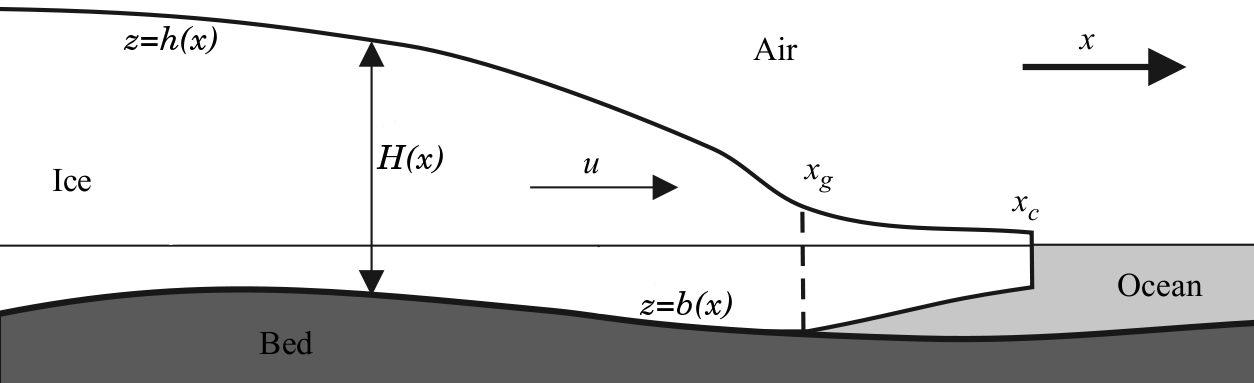
\includegraphics[width=6.0in]{flowline}
  
    \scriptsize \emph{Illustrates the notation used in these notes.  Figure modified from \cite{SchoofMarine1}.} \normalsize
    
    \vspace{1.5in}
  \end{center}
\end{titlepage}

\clearpage\newpage

%\setcounter{section}{1}
\section{Introduction}

The greatest importance of numerical models in glaciology is introspective.  You should ask yourself: When I combine my imperfect and incomplete understanding of glacier processes into this mathematical model which I put on a computer, does it behave as I expect?  Numerical models can indeed show how processes interact to give overall behavior.  They can at least demonstrate flaws in our understanding of those processes.  But they should be built with care.  An avoidable bad outcome is to spend time---or worse, reputation---interpreting, explaining, or justifying numerical model behavior that is in fact an artifact of poor computer programming or numerical analysis.

So the reader of these notes may be surprised that a continuum model, and not a computer code, seems to be our focus much of the time.  While all codes produce some numbers, we want numbers that actually come from the continuum model we have written down.  We will therefore analyse numerical implementations to see if they match the model equations and their solutions.

These notes have a limited scope:
  \begin{quote}\emph{shallow approximations of ice flow.}\end{quote}
They adopt a constructive approach; we provide:
  \begin{quote}\emph{example numerical codes that actually work.}\end{quote}
Within our scope are the shallow ice approximation (SIA) in two horizontal dimensions (2D), the shallow shelf approximation (SSA) in 1D, and the mass continuity and surface kinematical equations.  We recall the Stokes model, but we do not address its numerical solution.  Our numerical concepts include finite difference schemes, solving algebraic systems from stress balances, and the verification of codes using exact solutions.

Our notation, which generally follows \cite{GreveBlatter2009}, is common in the glaciological literature, but see Table \ref{tab:notation}.  Cartesian coordinates are $x,y,z$ with $z$ positive-upward.  If these coordinates or time $t$ appear as subscripts then they denote partial derivatives: $u_x = \partial u/\partial x$.  Tensor notation uses subscripts from the list $\{1,2,3,i,j\}$.  For example, ``$\tau_{ij}$'' or ``$\tau_{13}$'' denote entries of the deviatoric stress tensor.

These notes are based on nineteen Matlab codes, each about one-half page.  All have been tested in Matlab and Octave.  They are distributed by cloning the repository at
\begin{quote}
\url{https://github.com/bueler/mccarthy}
\end{quote}
\noindent and looking in the \texttt{mfiles/} subdirectory.  Five of these codes are printed here, with their comments stripped for compactness and clarity.  The electronic versions have generous comments and help files.

\begin{table}[ht]
\caption{Notation used in these notes, with values for some constants.}
\begin{tabular}{clll}
variable  & description & SI units & value \\
\hline
$A$ & $A=A(T)=$ ice softness in the Glen flow law & $\text{Pa}^{-n}\,\text{s}^{-1}$ \\
$B$ & ice hardness; $B=A^{-1/n}$ & $\text{Pa}\,\text{s}^{1/n}$ \\
$b$ & bedrock elevation & m \\
$c$ & specific heat in general & J kg$^{-1}$ K$^{-1}$ \\
$\nabla$ & (spatial) gradient & m$^{-1}$ \\
$\nabla\cdot$ & (spatial) divergence & m$^{-1}$ \\
$\mathbf{g}$ & gravity & m s$^{-2}$\phantom{foobar} & 9.81 \\
$H$ & ice thickness & m \\
$h$ & ice surface elevation & m \\
$\kappa$ & conductivity in general & J s$^{-1}$ m$^{-1}$ K$^{-1}$ \\
$M$ & climatic mass balance & m s$^{-1}$ \\
$n$ & exponent in Glen flow law & & 3 \\
$\nu$ & viscosity & Pa s \\
$p$ & pressure & Pa \\
$\bq$ & map-plane ice flux: $\bq = \int_{b}^{h} \bU\,dx = \bar{\bU} H$ & $\text{m}^2\,\text{s}^{-1}$ \\
$\rho$ & density of ice & kg m$^{-3}$ & 910 \\
$\rho_w$ & density of sea water & kg m$^{-3}$ & 1028 \\
$T$ & temperature & K \\
$\tau$ & norm (second invariant) of $\tau_{ij}$: $2 \tau^2 = \sum_{ij} \tau_{ij}^2$ & Pa \\
$\tau_{ij}$ & deviatoric stress tensor & Pa \\
$Du_{ij}$ & strain rate tensor & s$^{-1}$ \\
$\mathbf{U}$ & $=(u,v)$ horizontal ice velocity & m s$^{-1}$ \\
$\mathbf{u}$ & $=(u,v,w)$ 3D ice velocity & m s$^{-1}$ \\
\end{tabular}
\label{tab:notation}
\end{table}


\section{Ice flow equations}

My first goal in these notes is to get to an equation for which I can say:
\begin{center}
\emph{by numerically solving this equation, we have a usable model for an ice sheet.}
\end{center}
\noindent A ``usable'' model tends to be \emph{understood} as much as it is \emph{correct}.  Also, this first usable model will not be complete by any modern standard.  To get to my goal I first (briefly!) recall the continuum mechanical equations of ice flow.

Ice in glaciers is a moving fluid so we describe its motion by a velocity field $\mathbf{u}(t,x,y,z)$.  If the ice fluid were faster-moving than it actually is, and if it were linearly-viscous like liquid water, then it would be a ``typical'' incompressible fluid.  We would use the Navier-Stokes equations as the model:
\begin{align}
\nabla \cdot \mathbf{u} &= 0 &&\text{\emph{incompressibility}} \label{incompressible} \\
\rho \left(\mathbf{u}_t + \mathbf{u}\cdot\nabla \mathbf{u}\right) &= -\nabla p + \nabla \cdot (\nu \nabla \mathbf{u}) + \rho \mathbf{g} &&\text{\emph{stress balance}} \label{navierstokes}
\end{align}
In equation \eqref{navierstokes} the term $\mathbf{u}_t + \mathbf{u}\cdot\nabla \mathbf{u}$ is an acceleration.  The right-hand side of \eqref{navierstokes} is the total stress, and so equation \eqref{navierstokes} says ``$ma=F$'', i.e.~it is Newton's second law.  Much time has been spent to get partial understanding of the rich solutions of these Navier-Stokes equations; a book-length introduction like \cite{Acheson} is recommended.  The numerical solution of these equations is \emph{computational fluid dynamics} (CFD).

But, is ice flow modelling a part of CFD?  (And does a well-written general-purpose CFD text like \cite{Wesseling} help the glaciers student?)  It is true that ice sheet flow can be a large-scale fluid problem like atmosphere and ocean circulation in climate systems, but it is an odd one.  Consider some topics which might make ocean circulation modelling exciting, for example:
  \begin{center} turbulence \qquad convection \qquad  coriolis force  \qquad density stratification
  \end{center}
None of these topics are relevant to ice flow.  What could be interesting about the flow of slow, and surely boring, ice?

First observe that ice is indeed a slow fluid.  In terms of equation \eqref{navierstokes}, ``slow'' means $\rho \left(\mathbf{u}_t + \mathbf{u}\cdot\nabla \mathbf{u}\right) \approx 0$, which says that the forces (stresses) of inertia are negligible.  However, ice is also a shear-thinning fluid with a specific kind of nonlinearly-viscous (``non-Newtonian'') behavior in which larger shear strain rates imply smaller viscosity.  The viscosity $\nu$ in \eqref{navierstokes} is therefore not constant, and so we must separately state an empirically-based flow law in addition to restating \eqref{navierstokes} for slow flows.

\subsection*{Stokes equations}  The standard model for isothermal ice flow is this set of equations:
\begin{align}
\nabla \cdot \mathbf{u} &= 0 &&\text{\emph{incompressibility}} \label{incompressibleagain} \\
0 &= - \nabla p + \nabla \cdot \tau_{ij} + \rho \mathbf{g} &&\text{\emph{stress balance}} \label{forcebalance} \\
Du_{ij} &= A \tau^2 \tau_{ij} &&\text{\emph{$n$=3 Glen flow law}} \label{flowlaw}
\end{align}
In the flow law \eqref{flowlaw}, the deviatoric stress tensor $\tau_{ij}$ and the strain rate tensor $Du_{ij}$ appear; previous lectures cover these.  Here we merely note that: $Du_{ij} = (1/2)((u_i)_{x_j}+(u_j)_{x_i})$ if we index coordinates by $x_1,x_2,x_3=x,y,z$, each tensor in \eqref{flowlaw} is symmetric and has trace zero, and $\tau^2 = (1/2) \tau_{ij} \tau_{ij}$ (using the summation convention).

The Stokes equations do not contain a time derivative.  Thus boundary stresses, the force of gravity $\rho \mathbf{g}$, and ice softness $A$ together determine the velocity and stress fields (i.e.~$\bu$, $p$, $\tau_{ij}$) instantaneously.  Thus ice flow simulation codes have no memory of prior momentum or velocity.  Said another way, velocity is a ``diagnostic'' output of ice flow codes, because it is not needed for (re)starting a simulation.

\subsection*{Plane-flow Stokes equations}  Consider now the $x,z$-plane case of equations \eqref{incompressibleagain}, \eqref{forcebalance}, and \eqref{flowlaw}.  ``Plane-flow'' means that velocity component $v$ is zero and that all derivatives with respect to $y$ are zero:
\begin{align}
u_x + w_z &= 0 &&\text{\emph{incompressibility}} \label{incompressiblexz} \\
p_x &= \tau_{11,x} + \tau_{13,z} &&\text{\emph{stress balance} ($x$)} \label{stokespx} \\
p_z &= \tau_{13,x} - \tau_{11,z} - \rho g &&\text{\emph{stress balance} ($z$)} \label{stokespz} \\
u_x &= A \tau^2 \tau_{11} &&\text{\emph{flow law} (diagonal)}  \label{forceflowx} \\
u_z + w _x &= 2 A \tau^2 \tau_{13} &&\text{\emph{flow law} (off-diagonal)} \label{forceflowz}
\end{align}
Note that $\tau_{13}$ is a shear stress while $\tau_{11}$ and $\tau_{33}=-\tau_{11}$ are deviatoric longitudinal stresses.  Also $\tau^2 = \tau_{11}^2+\tau_{13}^2$ in this case.  Equations \eqref{incompressiblexz}--\eqref{forceflowz} form a system of five nonlinear equations in five scalar unknowns ($u,w,p,\tau_{11},\tau_{13}$).

\subsection*{Slab-on-a-slope}  Equations \eqref{incompressiblexz}--\eqref{forceflowz} are complicated enough to make us pause before jumping in to numerical solution methods, but  we can handle a simplified situation first.  A uniform slab of ice, or a ``slab-on-a-slope'', is both a case in which we can actually solve the Stokes equations, and a motivation for the shallow model in the next subsection.

\onefig{slab}{Rotated axes for a slab-on-a-slope flow calculation.}

We rotate our coordinates only for this example and not elsewhere in these notes.  The two-dimensional axes ($x$,$z$) shown in Figure \ref{fig:slab} are rotated downward (clockwise) at angle $\alpha>0$ so that the gravity vector has components $\mathbf{g} = (g \sin\alpha,- g \cos \alpha)$.  Equations \eqref{stokespx} and \eqref{stokespz} in these rotated coordinates are
\begin{align}
p_x &= \tau_{11,x} + \tau_{13,z} + \rho g \sin\alpha, \label{stokespxrot} \\
p_z &= \tau_{13,x} - \tau_{11,z} - \rho g \cos\alpha. \label{stokespzrot}
\end{align}
Assuming also that there is no variation with $x$, the whole set of Stokes equations \eqref{incompressiblexz}, \eqref{forceflowx}, \eqref{forceflowz}, \eqref{stokespxrot}, \eqref{stokespzrot} simplifies greatly:
\begin{align}
w_z &= 0 &   0 &= \tau_{11} \label{stokesslab} \\
\tau_{13,z} &= - \rho g \sin\alpha &   u_z &= 2 A \tau^2 \tau_{13} \notag \\
p_z &= -\tau_{11,z} = - \rho g \cos\alpha \notag
\end{align}
We apply boundary conditions for these functions of $z$: $w(0)=0$, $p(H)=0$, $u(0)=u_0$.  The basal velocity $u_0$ will remain undetermined for now.

By integrating equations \eqref{stokesslab} with respect to $z$, and using $\tau_{11}=0$, we get $w=0$, $p = \rho g \cos\alpha (H-z)$, and $\tau_{13} = \rho g \sin\alpha (H-z)$.  Note that $H-z$ is the depth below the ice surface, so both the pressure $p$ and shear stress $\tau_{13}$ are proportional to depth.  Because $u_z = 2 A \tau^2 \tau_{13}$, by integrating vertically again we find the horizontal velocity:
\begin{align}
u &= u_0 + \frac{1}{2} A (\rho g \sin\alpha)^3  \left(H^4 - (H-z)^4\right)  \label{uslab}
\end{align}

Do we believe formula \eqref{uslab}?  Figure \ref{fig:slabvel} compares it to observations of a mountain glacier, and it shows we have already done a credible job of capturing deformation flow velocity in this case.  We do not yet have a model for the sliding velocity $u_0$ (i.e.~basal motion).  

\twofigsizes{slabvel}{athabasca-deform}{Left:  Velocity from slab-on-a-slope formula \eqref{uslab}.  Right:  Inclinometry-measured velocity in a glacier (Athabasca Glacier \cite{SavagePaterson}).}{2.0in}{1.8in}

\subsection*{Plane-flow mass-continuity equation}  Observe that the equations so far do not address the change in shape of the glacier or ice sheet.  For this we need another equation, the \emph{mass continuity equation}.  We consider the general case of an $x,z$-plane flow with variable thickness and velocity, not just slab-on-a-slope.  Define the vertical average of the horizontal velocity:
	$$\bar U = \frac{1}{H}\int_0^{H} u\,dz.$$
The flux $q=\bar U\, H = \int_0^{H} u\,dz$ is the rate of flow input into the side of the area in Figure \ref{fig:slabmasscontfig}.

\onefigsize{slabmasscontfig}{Mass continuity equation \eqref{masscont1D} follows from considering the changing area $A$ of ice in a planar flow.  Ice can be added by surface mass balance $M$ or a difference of flux $q=\bar u H$ into the left and right sides.}{2.5in}

The ice area $A$ in Figure \ref{fig:slabmasscontfig} changes according to the sum of all the boundary contributions,
\begin{equation}
\frac{dA}{dt} = \int_{x_1}^{x_2} M(x)\,dx + \bar U_1 H_1 - \bar U_2 H_2: \label{masscontintegrated}
\end{equation}
Here $M(x)$ is the climatic mass balance at the ice surface.  (In three-dimensions, equation \eqref{masscontintegrated} would become an equation for $dV/dt$, the rate of change of ice volume.)

If the width $\Delta x=x_2-x_1$ is small then $A\approx \Delta x\, H$.  So we divide by $\Delta x$ and take $\Delta x \to 0$ in \eqref{masscontintegrated} and get
\begin{equation}
H_t = M - \left(\bar U H\right)_x \label{masscont1D}
\end{equation}
This mass continuity equation describes change in the ice thickness in terms of surface mass balance and ice velocity.  An important aspect of ice flow simulations is how one computes the velocity which goes into this equation.

\subsection*{Viscosity form of the flow law}  The flow law \eqref{flowlaw} has another form which we will use next, and also later in describing ice shelf and stream flow.  Recall $\tau^2 = (1/2) \tau_{ij} \tau_{ij}$ and also define $|Du|^2 = (1/2) Du_{ij} Du_{ij}$.  The scalars $\tau$ and $|Du|$ are norms (also ``second invariants'') of the tensors $\tau_{ij}$ and $Du_{ij}$, respectively.  By taking these norms of both sides of \eqref{flowlaw} we get $|Du| = A \tau^3$.  But then $\tau = A^{-1/3} |Du|^{1/3}$, so \eqref{flowlaw} can be rewritten
\begin{equation}
\tau_{ij} = 2 \nu\, Du_{ij}  \qquad \text{\emph{flow law (viscosity form)}} \label{viscosityflowlaw}
\end{equation}
where $\nu = (1/2) A^{-1/3} |Du|^{-2/3}$ is the nonlinear viscosity.  Often $B = A^{-1/3}$ is called the ice ``hardness''.  The derivation of \eqref{viscosityflowlaw} is worth knowing in detail; see the Exercises.

Form \eqref{viscosityflowlaw} of the flow law allows us to eliminate stresses $\tau_{ij}$ from the Stokes equations by replacing them with formulas depending on derivatives of the velocity.  That is, one can write the Stokes equations in terms of the strain rates only.  The next two approximate models also use this idea.

\subsection*{The Blatter-Pattyn approximation}  We return now briefly to plane-flow Stokes equations \eqref{incompressiblexz}--\eqref{forceflowz}, and reconsider how to simplify them.  One simplification step, present in all shallow models, is to drop the single term  $\tau_{13,x}$ from the $z$-component of the stress balance \eqref{stokespz}.  This assumes that horizontal variation in the vertical shear stress is small compared to the other terms:
\begin{equation}
p_z = - \tau_{11,z} - \rho g. \label{hydrostaticpz}
\end{equation}
Because the (Cauchy) stress tensor $\sigma_{ij}$ is related to the deviatoric stress tensor by $\sigma_{ij} = \tau_{ij} - p \delta_{ij}$, and thus $p + \tau_{11} = p - \tau_{33} = - \sigma_{33}$, equation \eqref{hydrostaticpz} says that the vertical normal stress $\sigma_{33}$ is linear in depth; this is similar to a statement that the ice is hydrostatic.  Taking it to have surface value zero we get
\begin{equation}
p + \tau_{11} = \rho g (h-z). \label{hydrostaticitself}
\end{equation}

Equation \eqref{hydrostaticitself} allows one to eliminate $p$ from the model equations.  Furthermore, taking the $x$-derivative of \eqref{hydrostaticitself} and substituting into \eqref{stokespx}, then using the viscosity form \eqref{viscosityflowlaw}, leads to this equation (Notes and References and \cite{GreveBlatter2009}):
\begin{equation}
\left(4 \nu u_x\right)_x + \left(\nu (u_z+w_x)\right)_z = \rho g h_x \qquad\text{\emph{hydrostatic stress balance}} \label{stresshydrostatic}
\end{equation}
The hydrostatic stress balance equation \eqref{stresshydrostatic} is nontrivially-coupled to incompressibility \eqref{incompressiblexz} because derivatives of the vertical velocity $w$ appear in both equations, though $p$ is gone.  Nonetheless coupled equations \eqref{incompressiblexz} and \eqref{stresshydrostatic}, along with the formula $\nu = (1/2) A^{-1/3} |Du|^{-2/3}$ and appropriate boundary conditions, determine $u$ and $w$.

If we drop $w_x$ from equation \eqref{stresshydrostatic} then we get the Blatter-Pattyn model:
\begin{equation}
\left(4 \nu u_x\right)_x + \left(\nu u_z\right)_z = \rho g h_x \qquad\text{\emph{Blatter-Pattyn stress balance}} \label{stressblatter}
\end{equation}
Using this equation one can solve first for the horizontal velocity $u$ and then afterward recover $w$ from \eqref{incompressiblexz}; stress balance and incompressibility are decoupled.

\section{Shallow ice sheets}

Ice sheets have four outstanding properties as fluids.  They are (\emph{i}) slow, (\emph{ii}) shallow,  (\emph{iii}) non-Newtonian, and (\emph{iv}) they experience some contact slip (basal sliding).  The first ice flow model which we solve numerically in these notes is the non-sliding, isothermal \emph{shallow ice approximation} (SIA).  It accounts for (\emph{i})--(\emph{iii}).

Regarding the property of shallowness, Figure \ref{fig:green-transect} shows both a no-vertical-exaggeration cross-section of Greenland at $71^\circ$, as well as the standard vertically-exaggerated version which is more familiar in the glaciological literature.  In other words, ice sheets \emph{are} shallow, though of course the portion of an ice sheet which you want to model may not be.

\onefig{green-transect}{A vertically-exaggerated cross-section of the Greenland ice sheet ($71^\circ$ N) is shown by the upper two curves.  Without exaggeration it appears as merely a thickened horizontal line.}

Our slab-on-a-slope example gives us a rough explanation of the SIA.  To show the SIA in its plane-flow form, we vertically integrate velocity formula \eqref{uslab} in the $u_0=0$ (non-sliding) case to get
\begin{equation}
\bar u H = \int_0^H \frac{1}{2} A (\rho g \sin\alpha)^3  \left(H^4 - (H-z)^4\right)\,dz = \frac{2}{5} A (\rho g \sin\alpha)^3 H^5. \label{siaubar}
\end{equation}
Note $\sin \alpha \approx \tan\alpha = - h_x$.  Combining these statements with mass continuity \eqref{masscont1D} gives
\begin{equation}
  H_t = M + \left(\frac{2}{5} (\rho g)^3 A H^5 |h_x|^2 h_x\right)_x. \label{sia1D}
\end{equation}

Equation \eqref{sia1D} is the SIA equation for nonsliding plane flow.  It is the promised first usable model for the evolution of an ice sheet's thickness $H$ in terms of surface mass balance $M$, ice softness $A$, and bed elevation $b$ (because $h=H+b$).  The model must, however, be solved subject to the constraint that the thickness is positive ($H\ge 0$); see Notes and References.

Additional arguments are needed to demonstrate that the SIA is more general-purpose than the special case of a simple slab; see Notes and References.  Such arguments reduce the Stokes equations under the assumption that the surface and bed slopes, and the depth-to-width ratio, are small.

We will numerically solve the SIA in section \ref{sec:numericalsia}, but first we state it in two horizontal dimensions.  Let $\mathbf{U} = (u,v)$ be the vector horizontal velocity.  The shear stress approximation is $(\tau_{13},\tau_{23}) \approx - \rho g (h-z) \nabla h$, which appeared as ``$\tau_{13}= \rho g \sin \alpha (h-z)$ and $\sin \alpha \approx -h_x$'' in the previous section, becomes an equality in the SIA.  Equation \eqref{flowlaw} then gives the SIA formula for shear strain rates
\begin{equation*}
\mathbf{U}_z = 2 A |(\tau_{13},\tau_{23})|^{n-1} (\tau_{13},\tau_{23}) = - 2 A (\rho g)^n (h-z)^n |\nabla h|^{n-1} \nabla h.
\end{equation*}
By integrating vertically we get, in the non-sliding case,
\begin{equation}
\mathbf{U} = - \frac{2 A (\rho g)^n}{n+1} \left[H^{n+1} - (h-z)^{n+1}\right] |\nabla h|^{n-1} \nabla h.  \label{siavelocity}
\end{equation}

Mass continuity in two horizontal dimensions, which generalizes the 1D version \eqref{masscont1D}, also applies:
\begin{equation}
    H_t = M - \Div\left(\bar{\mathbf{U}} H\right)  \label{masscont}
\end{equation}
Equation \eqref{masscont} may be written $H_t = M - \Div \bq$ in terms of the map-plane flux $\bq = \int_{b}^{h} \mathbf{U}\,dz = \bar{\mathbf{U}}\,H$.

Combining Equations \eqref{siavelocity} and \eqref{masscont}, we get an equation for the rate of thickness change in terms of mass balance $M$, thickness, and surface slope $\grad h$:
\begin{equation}
H_t = M + \Div \left(\Gamma H^{n+2} |\grad h|^{n-1} \grad h \right), \label{sia}
\end{equation}
where we have defined the positive constant $\Gamma = 2 A (\rho g)^n / (n+2)$.  Equation \eqref{sia} is the SIA in two dimensions.  Recalling our earlier promise, if we can solve \eqref{sia} numerically then we have, following Mahaffy \cite{Mahaffy}, a usable model for the Barnes ice cap in Canada, a particularly-simple ice sheet on a rather flat bed.

\subsection*{Analogy with the heat equation}  The SIA model is easy to compare with the better-known heat equation.  Numerical methods for solving \eqref{sia} can be understood as modifications of well-known heat equation methods.

In the simplest one-dimensional (1D) case, the heat equation for the temperature $T(t,x)$ of a conducting rod is
\begin{equation}
  T_t = D T_{xx}. \label{heat1D}
\end{equation}
This form applies when material properties are constant and there are no heat sources.  The positive constant $D$ is the ``diffusivity,'' with units which can be read from comparing sides of the equation: $D\sim \text{m}^2 \text{s}^{-1}$.  Observe that equation \eqref{heat1D} has a smoothing effect on the solution $T$ as it evolves in time, because any local maximum in the temperature is flattened (i.e.~$T_{xx}<0$ implies $T_t<0$ so $T$ decreases), while any local minimum is also flattened (i.e.~$T_{xx}>0$ implies $T_t>0$ so $T$ increases).

We will state the 2D heat equation more generally.  It describes the temperature $T(t,x,y)$ of some planar object, at position $x,y$ and time $t$.  Recall that Fourier's law for conduction is the formula $\mathbf{Q} = - \kappa \grad T$ for heat flux $\mathbf{Q}$, where $\kappa$ is conductivity.  We will assume, for the purposes of our analogy, that $\kappa(x,y)$ may vary in space.  Also suppose there is a variable heat source $f(t,x,y)$, with units of Watts per cubic meter.  Then conservation of internal energy says
\begin{equation}
\rho c T_t = f + \Div (\kappa \grad T). \label{heatearly}
\end{equation}
Here $\rho$ is density and $c$ is specific heat capacity.  Assuming $\rho c$ is constant, define the ``diffusivity'' $D=\kappa/(\rho c)$ and the rescaled source term $F = f/(\rho c)$.  The revised 2D heat equation is
\begin{equation}
T_t = F + \Div (D\, \grad T). \label{heat}
\end{equation}
It clearly generalizes equation \eqref{heat1D}.

Figure \ref{fig:initialheat} shows a solution of heat equation \eqref{heat}, wherein the initial condition is a localized ``hot spot''.  Solutions of the heat equation always involve the spreading, in all directions, of any local heat maxima or minima, that is, diffusion.

\twofigsizes{initialheat}{finalheat}{A solution of heat equation \eqref{heat} with $D=1$ and $F=0$.  Left: Initial condition $T(0,x,y)$.   Right: Solution $T(t,x,y)$ at $t=0.02$.}{2.8in}{2.8in}

The SIA equation \eqref{sia} and the heat equation \eqref{heat} are each diffusive, time-evolving partial differential equations (PDEs).  A side-by-side comparison is illuminating:
\begin{center}
\begin{tabular}{cc}
\vspace{1mm}
SIA:\, $H$ is ice thickness & \phantom{foo bar} heat: $T$ is temperature\phantom{foo bar}  \\
\vspace{1mm}
	$H_t = M + \Div \left({\color{red}\Gamma H^{n+2} |\grad h|^{n-1}}\, \grad h \right)$  &  $T_t = F + \Div (D\, \grad T)$
\end{tabular}
\end{center}
\vspace{1mm}
Notice that the number of derivatives (one time and two space derivatives) and the signs are the same.  Surface mass balance $M$ is analogous to heat source $F$.  

The analogy suggests that we identify the \emph{diffusivity in the SIA} as:
\begin{equation}
	D = {\color{red}\Gamma H^{n+2} |\grad h|^{n-1}}.  \label{siadiffusivity}
\end{equation}
A non-sliding SIA flow diffuses the thickness of the ice sheet, and when this $D$ comes out large then the diffusion acts most quickly.  Being a product of $\Gamma$ and the powers of $H$ and $|\grad h|$, this diffusivity $D$ is large if the ice is both thick and steep.  In summary, ice diffuses (i.e.~flows downhill) more when it is thick and steep.

This diffusion equation analogy explains generally why the surfaces of ice sheets are smooth, at least if we overlook non-flow processes like crevassing and wind-driven (snow) dunes.  There are, however, some practical and conceptual issues with the analogy:
\begin{itemize}
\item The diffusivity $D$ in \eqref{siadiffusivity} depends on the solution, both thickness $H$ and surface slope $|\grad h|$.  This affects how we reason about diffusivity.  Numerical solution processes are more difficult because nonlinear equations are harder to solve.
\item The diffusivity $D$ in \eqref{siadiffusivity} goes to zero at margins, where $H\to 0$, and at divides and domes, where $|\grad h|\to 0$.  This means that the solution is not smooth, even though the thickness is continuous everywhere (and zero outside the ice sheet).  A non-smooth solution generates larger numerical errors.
\end{itemize}
More important is a deficiency of the SIA model, and not the analogy \emph{per se}, namely
\begin{itemize}
\item Ice flow is much less diffusive when significant longitudinal (membrane) stresses are present, as when ice is floating or sliding or when the flow is confined by terrain.
\end{itemize}
Nonetheless we continue toward a verified numerical scheme for the SIA model \eqref{sia} (Section \ref{sec:numericalsia}).  The next Section introduces some numerical PDE methods in general.

\section{Finite difference numerics} 

The diffusivity analogy above suggests that numerical schemes for the heat equation are a starting point for solving the SIA equation \eqref{sia}.  Here we demonstrate only finite difference (FD) schemes, in which we replace derivatives by mere arithmetic.

The basic fact on which FD schemes are based is \emph{Taylor's theorem}, which says that for a smooth function $f(x)$,
	$$f(x+\Delta) = f(x) + f'(x) \Delta + \frac{1}{2} f''(x) \Delta^2 + \frac{1}{3!} f'''(x) \Delta^3 + \dots$$
You can replace ``$\Delta$'' by its multiples, for example:
\begin{align*}
f(x+2\Delta) &= f(x) + 2 f'(x) \Delta + 2 f''(x) \Delta^2 + \frac{4}{3} f'''(x) \Delta^3 + \dots \\
f(x-\Delta) &= f(x) - f'(x) \Delta + \frac{1}{2} f''(x) \Delta^2 - \frac{1}{3!} f'''(x) \Delta^3 + \dots
\end{align*}
The idea for constructing FD schemes is to combine expressions like these to give approximations of derivatives.  Thereby an equation relating values on a grid serves to approximate the differential equation.

Here we want partial derivative approximations, so we apply the Taylor's expansions one variable at a time.  For example, with a general function $u=u(t,x)$,
\begin{align*}
u_t(t,x) &= \frac{u(t+\Delta t,x) - u(t,x)}{\Delta t} + O(\Delta t), \\
u_t(t,x) &= \frac{u(t+\Delta t,x) - u(t-\Delta t,x)}{2\Delta t} + O((\Delta t)^2), \\
u_x(t,x) &= \frac{u(t,x+\Delta x) - u(t,x-\Delta x)}{2\Delta x} + O((\Delta x)^2), \\
u_{xx}(t,x) &= \frac{u(t,x+\Delta x) - 2\, u(t,x) + u(t,x-\Delta x)}{\Delta x^2} + O((\Delta x)^2)
\end{align*}
Note that if $\Delta$ is a small number then ``$+O(\Delta^2)$'' is smaller than ``$+O(\Delta)$'', so the approximation is closer when you drop it.

\subsection*{Explicit scheme for the heat equation}  We first build the simplest ``explicit'' scheme which approximates the 1D heat equation \eqref{heat1D}.  It is based on the fact that because $T_t$ and $D T_{xx}$ are equal, these two FD expressions are nearly equal:
\begin{equation}
\frac{T(t+\Delta t,x) - T(t,x)}{\Delta t} \approx D\,\frac{T(t,x+\Delta x) - 2\, T(t,x) + T(t,x-\Delta x)}{\Delta x^2}.  \label{heat1Dapproximated}
\end{equation}
The scheme itself is a method for computing numbers on a grid.  That is, \eqref{heat1Dapproximated} approximates the PDE, but making it into an equality tells how to \emph{determine} grid values.

Let $(t_n,x_j)$ denote the points of the time-space grid shown in Figure \ref{fig:timespacegrid}.  Denote our approximation of the solution value $T(t_n,x_j)$ by $T_j^n$.  Then the finite difference scheme is
	$$\frac{T_j^{n+1} - T_j^n}{\Delta t} = D\,\frac{T_{j+1}^n - 2\, T_j^n + T_{j-1}^n}{\Delta x^2}.$$
To get a computable formula, let $\mu = D \Delta t / (\Delta x)^2$ and solve for $T_j^{n+1}$:
\begin{equation}
  T_j^{n+1} = \mu T_{j+1}^n + (1 - 2 \mu) T_j^n + \mu T_{j-1}^n \label{heat1Dfd}
\end{equation}

\onefigsize{timespacegrid}{A grid for a finite difference solution to \eqref{heat1D}.}{2.0in}

FD scheme \eqref{heat1Dfd} is \emph{explicit} because it directly computes $T_j^{n+1}$ in terms of values at time $t_n$.  Figure \ref{fig:expstencil} (left) shows the ``stencil'' for scheme \eqref{heat1Dfd}: three values at the current time $t_n$ are combined to update the one value at the next time $t_{n+1}$.

Before moving on, notice that evaluating a heat equation solution at a grid point (i.e.~the expression ``$T(t_n,x_j)$'') is generally a different number from the value $T_j^n$ computed by a scheme like \eqref{heat1Dfd}.  We intend that the numbers $T(t_n,x_j)$ and $T_j^n$ become closer together as the grid is made finer (i.e.~$\Delta t \to 0$ and $\Delta x \to 0$), because the FD expressions become closer to the derivatives they approximate.  That is, we intend our FD scheme to \emph{converge} under \emph{grid refinement}.  For now we \emph{plan} and \emph{hope} that convergence happens, but it needs checking (``verification''; Section \ref{sec:exactsolutions}) or perhaps a proof.

\twofigsizes{expstencil}{exp2dstencil}{Left: Space-time stencil for the explicit scheme \eqref{heat1Dfd} for the 1D heat equation.  Right: Spatial-only stencil for scheme \eqref{heat2dexplicit}.}{2.0in}{2.1in}

How accurate is scheme \eqref{heat1Dfd}?  Its construction tells us that the difference between the scheme \eqref{heat1Dfd} and the PDE \eqref{heat1D} is $O(\Delta t + (\Delta x)^2)$, so this difference goes to zero as we refine the grid in space and time, a property called \emph{consistency}.  With care about the smoothness of boundary conditions, and using mathematical facts about the heat equation itself, one can show that the difference between $T_j^n$ and $T(t_n,x_j)$ is also $O(\Delta t + (\Delta x)^2)$, which is thus the \emph{convergence rate}; see Notes and References.

To get convergence the PDE problem must generate adequately smooth solutions, and also scheme \eqref{heat1Dfd} must be \emph{stable}, which we address below.  The main theorem for numerical PDE schemes is ``consistency plus stability implies convergence''; see Notes and References.  Instead of pursuing such theory, however, these notes we do something rather practical, namely verification.  We find problems for which we already know an exact solution $T(t,x)$, and then we compute the differences $|T_j^n - T(t_n,x_j)|$.  This determines directly whether our actual \emph{implementation} (i.e.~computer code form of the scheme) actually does converge, not just whether it should in theory.

\subsection*{A first implemented scheme}  Our first Matlab implementation is for the 2D Equation \eqref{heat} with $D$ constant and $F=0$:
\begin{equation}
T_t = D (T_{xx}+T_{yy}).\label{heat2D}
\end{equation}
Writing $T_{jk}^n \approx T(t_n,x_j,y_k)$, the 2D explicit scheme is
\begin{equation}
	\frac{T_{jk}^{n+1} - T_{jk}^n}{\Delta t} = D\,\left(\frac{T_{j+1,k}^n - 2\, T_{jk}^n + T_{j-1,k}^n}{\Delta x^2} + \frac{T_{j,k+1}^n - 2\, T_{jk}^n + T_{j,k-1}^n}{\Delta y^2}\right). \label{heat2dexplicit}
\end{equation}
The stencil for the right-hand side of \eqref{heat2dexplicit} is shown in Figure \ref{fig:expstencil} (right).

Scheme \eqref{heat2dexplicit} has implementation \texttt{heat.m} below.  For simplicity we set $T=0$ on the boundary of the square $-1 < x < 1$, $-1 < y < 1$.  The initial condition is gaussian: $T(0,x,y) = \exp(-30 (x^2+y^2))$.  The code uses Matlab ``colon'' notation to remove loops over spatial variables.  Here is an example run:
\begin{Verbatim}
>>  heat(1.0,30,30,0.001,20);
\end{Verbatim}
This sets $D=1.0$ and uses a $30\times 30$ spatial grid.  We take $N=20$ time steps of $\Delta t = 0.001$.  The result is shown in Figure \ref{fig:initialheat}, right.  This is the look of success.

\minput{heat}

However, very similar runs seem to succeed or fail according to some as-yet unclear circumstances.  For example, results from these calls are shown in Figure \ref{fig:stability}:
\begin{Verbatim}
>> heat(1.0,40,40,0.0005,100);    % Figure 8, left
>> heat(1.0,40,40,0.001,50);      % Figure 8, right
\end{Verbatim}
Both runs compute temperature $T$ on the same spatial grid, for the same final time $t_f = N \Delta t = 0.05$, but with different time steps.  Noting the vertical axes, the second run clearly shows ``instability,'' an extreme form of inaccuracy characterized in practice by numbers of a totally different magnitude than expected.

\twofig{stability}{instability}{Numerically-computed temperature on $40\times 40$ grids.  The two runs are the same except that the left has $\Delta t=0.0005$ so $D\Delta t/(\Delta x)^2= 0.2$, while the right has $\Delta t=0.001$ so $D\Delta t/(\Delta x)^2= 0.4$.  Compare \eqref{stabcrit}.}


\subsection*{Stability criteria and adaptive time stepping}  To avoid the instability shown at right in Figure \ref{fig:stability}, we need to understand the scheme better.  It turns out we have not made an implementation error.  Instead, care is required when choosing space and time steps.

Recall the 1D explicit scheme in form \eqref{heat1Dfd}: $T_j^{n+1} = \mu T_{j+1}^n + (1 - 2 \mu) T_j^n + \mu T_{j-1}^n$.  The new value $T_j^{n+1}$ is an average of the old values, in the sense that the coefficients add to one.  Averaging is stable because averaged wiggles are smaller than the wiggles themselves.  Actually, however, the scheme is only an average \emph{if} the middle coefficient is positive, as a linear combination with coefficients which add to one is not an average if any coefficients are negative.  (For example, one would not accept 15 as an ``average'' of 5 and 7, but: $15 = -4 \times 5 + 5 \times 7$, and $-4+5=1$.)

So, what follows from requiring the middle coefficient in \eqref{heat1Dfd} to be positive so it computes such an average?  A \emph{stability criterion} follows, with these equivalent forms:
\begin{equation}
   1 - 2 \mu \ge 0 \quad \iff \quad \frac{D\Delta t}{\Delta x^2} \le \frac{1}{2} \quad \iff \quad \Delta t \le \frac{\Delta x^2}{2 D}.  \label{stabcrit}
\end{equation}
The third form states the condition as a limitation on the size of $\Delta t$.  It is a \emph{sufficient} stability criterion; it is enough to guarantee stability, though something weaker might do.  In summary, for given $\Delta x$, shortening the time steps $\Delta t$ so that \eqref{stabcrit} holds will make FD scheme \eqref{heat1Dfd} into an averaging process.

Applying this same idea to the 2D heat equation \eqref{heat2D} leads to the stability condition that $1-2\mu^x-2\mu^y \ge 0$ where $\mu^x = D \Delta t / (\Delta x^2)$ and $\mu^y = D \Delta t / (\Delta y^2)$.  In the cases shown in Figure \ref{fig:stability}, wherein $\Delta x=\Delta y$, this condition requires $D \Delta t /(\Delta x^2) \le 0.25$.  This inequality precisely distinguishes between the two parts of Figure \ref{fig:stability}.

In summary, runs of \texttt{heat.m} are unstable if the time step $\Delta t$ is too big relative to the spacing $\Delta x$.  The stability criterion is, however, satisfied by making each time step shorter.  Enforcing the criterion inside the code itself is an \emph{adaptive} implementation.  Such an implementation can be stable even if the diffusivity $D$ is changing in time.  To show how easy this is to implement, \texttt{heatadapt.m} (not shown) is the same as \texttt{heat.m} except that the time step comes from the stability criterion.  However, if the diffusivity $D$ is large or the grid spacings $\Delta x$, $\Delta y$ are small, then adaptive explicit implementations must take many short time steps to assure stability.  Adaptive explicit schemes can be slow.


\subsection*{Implicit schemes}  There is an alternative stability fix instead of adaptivity, namely ``implicitness.''  For example, the finite difference scheme
\begin{equation}
  \frac{T_j^{n+1} - T_j^n}{\Delta t} = D\,\frac{T_{j+1}^{n+1} - 2\, T_j^{n+1} + T_{j-1}^{n+1}}{\Delta x^2} \label{implicit1D}
\end{equation}
is an $O(\Delta t + (\Delta x)^2)$ implicit scheme for Equation \eqref{heat1D}.  This implicit scheme for the heat equation is stable for \emph{any} positive time step $\Delta t>0$ (``unconditionally stable''); see Notes and References.  Another well-known implicit scheme is \emph{Crank-Nicolson}, which is unconditionally stable for the heat equation, but with smaller error $O((\Delta t)^2 +(\Delta x)^2)$.

Implicit schemes are harder to implement because the unknown solution values at time step $t_{n+1}$ are treated as a vector in a large system of equations which must be formed and solved at each time step.  If the PDE is nonlinear then the system of equations may be hard to solve.  Though the SIA is a highly nonlinear diffusion equation, implicit schemes are becoming useful \cite{Bueler2016}.  Because of the tradeoff between the easy implementability of adaptive explicit schemes and the better stability of implicit schemes, for these notes we stay with adaptive explicit (FD) schemes.

\subsection*{Numerical solution of diffusion equations}  We are trying to numerically model ice flows, not heat conduction.  We have an analogy, however, which says that the SIA is diffusive like the heat equation.  In this section, because we wish to solve the SIA on real bedrock, we construct a numerical scheme for a more general diffusion equation which has an extra ``shift'' inside the gradient, namely
\begin{equation}
  T_t = F + \Div \left(D \grad (T + b)\right). \label{gendiffusion}
\end{equation}
In equation \eqref{gendiffusion}, the source term $F(x,y)$, the diffusivity $D(x,y)$, and the ``shift'' $b(x,y)$ may all vary in space.

The following code solves \eqref{gendiffusion}.  It is called by the SIA-specific schemes we build next.

\minput{diffusion}

This adaptive explicit method for the diffusion equation is conditionally stable, with the same essential time step restriction as for the constant diffusivity case, as long as we evaluate $D(x,y)$ at \emph{staggered} grid points.  That is, we use this expression for the second derivative:
\begin{align*}
\Div \left(D \grad X\right) &\approx \frac{D_{j+1/2,k}(X_{j+1,k} - X_{j,k}) - D_{j-1/2,k}(X_{j,k} - X_{j-1,k})}{\Delta x^2} \\
	&\qquad + \frac{D_{j,k+1/2}(X_{j,k+1} - X_{j,k}) - D_{j,k-1/2}(X_{j,k} - X_{j,k-1})}{\Delta y^2},
\end{align*}
where $X=T+b$.  The left part of Figure \ref{fig:diffstencil} shows the stencil.

\twofigsizes{diffstencil}{mahaffystencil}{Left:  Spatial stencil for staggered grid evaluation of diffusivity (at triangles) in the diffusion equation \eqref{gendiffusion}.  Right: Stencil showing how the staggered-grid diffusivity (triangle) can be evaluated in the SIA, from surface elevation (diamonds) and thicknesses (squares).}{2.2in}{2.2in}

The user supplies the diffusivity $D(x,y)$ to \texttt{diffusion.m} on the staggered grid.  The initial temperature $T(0,x,y)$, source term $F(x,y)$, and ``shift'' $b(x,y)$ are also supplied on the regular grid.  When using this code for standard diffusions, or for the flat-bed case of the SIA, we would take $b=0$.


\section{Numerically solving the SIA} \label{sec:numericalsia}

In SIA equation \eqref{sia} we have diffusivity $D = \Gamma H^{n+2} |\grad h|^{n-1}$.  As already noted, an interesting aspects of this formula is that $D$ goes to zero, the diffusion ``degenerates,'' when either $H\to 0$ or $\grad h \to 0$.  Degenerate diffusion equations are automatically free boundary problems, but this aspect of the thickness evolution problem should be no surprise to a glaciologist.  Determining the location of the margin is an obvious part of modelling a glacier or ice sheet.  To address this free boundary issue in our explicit time-stepping code it suffices to numerically compute new thicknesses and then set them to zero if they come out negative.

Second, for numerical stability and mass conservation we should compute $D$ on a ``staggered'' grid.  Various finite difference schemes for computing it have been proposed.  All of these schemes involve averaging $H$ and differencing $h$ in a ``balanced'' way onto the staggered grid.  In the code \texttt{siaflat.m} below we use the Mahaffy \cite{Mahaffy} method, with the stencil for computing $D$ shown in Figure \ref{fig:diffstencil} (right).  This code only works for the flat bed, zero surface mass balance case, but we will correct these deficiencies later.

\minput{siaflat}


\section{Exact solutions and verification} \label{sec:exactsolutions}

In \texttt{siaflat.m}, which calls \texttt{diffusion.m}, we already have a fairly complicated code.  How do we make sure that such an implemented numerical scheme is correct?  Here are three proposed techniques:
\begin{enumerate}
  \item don't make any mistakes, or
  \item compare your numerical results with results from other researchers, and hope that the outliers are in error, or
  \item compare your numerical results to an exact solution.   \end{enumerate}
The first two of these, which one might call ``infallibility'' and ``intercomparison,'' respectively, should be less common approaches than they are.  The last one of these, preferred to the first two by the CFD community generally \cite{Wesseling}, is called ``verification.''

It is a simple idea:  When we build a new computer code we should test it in cases where we know the right answer.  To do so we need to return to the PDE itself, to get useful exact solutions.

\subsection*{Exact solution of heat equation}  First we return to the simpler case of the 1D heat equation with constant $D$, namely $T_t = D T_{xx}$.  Many exact solutions $T(t,x)$ to this heat equation are known, but let's consider the time-dependent ``Green's function,'' also known as the ``heat kernel''.  It starts at time $t=0$ with a delta function $T(0,x)=\delta(x)$ of heat at the origin $x=0$.  Then it spreads out over time.  It is a solution of the heat equation on the whole line $-\infty<x<\infty$ and for all $t>0$.

We will calculate this exact solution by a method which generalizes to the SIA.  In both cases the Green's function is ``self-similar'' over time, in the sense that it changes shape \emph{only} by shrinking the output (vertical) axis and lengthening the input (horizontal) axis, as shown in Figure \ref{fig:heatscaling} for the heat equation.  These scalings are related to each other by conservation of energy, which says that the total heat energy is independent of time.

\onefigsize{heatscaling}{The heat equation Green's function in 1D has the same shape at each time, but with time-dependent input- and output-scalings.}{2.4in}

The Green's function of the 1D heat equation is
  $$T(t,x) = (4 \pi D t)^{-1/2}\, e^{-x^2/(4Dt)}.$$
``Similarity'' variables for this solution, the above-mentioned scalings, involving multiplying the input and output of an invariant shape function $\phi(s) = (4 \pi D)^{-1/2}\, e^{-s^2/(4D)}$ by the same power of $t$:
\begin{equation}
s \stackrel{\text{\emph{input scaling}}}{\phantom{\Big|}=\phantom{\Big|}} t^{-1/2} x, \qquad\qquad T(t,x) \stackrel{\text{\emph{output scaling}}}{\phantom{\Big|}=\phantom{\Big|}} t^{-1/2} \phi(s).  \label{heatscalings}
\end{equation}

A numerical solver for the 1D heat equation which starts with initial values $T(t_0,x)$ taken from this exact solution should, at a later time $t$, produce numbers which are close to the exact solution $T(t,x)$; see the Exercises.

\subsection*{Halfar's similarity solution to the SIA}  Now we jump from Green's idea in about 1830 to the year 1981.  That is when P.~Halfar published the similarity solution of the SIA in the case of flat bed and zero surface mass balance.  Halfar's solution to the 2D SIA model \eqref{sia}, using a Glen exponent $n=3$, has scalings similar to \eqref{heatscalings} above:
\begin{equation}
s = t^{-1/18} r, \qquad \qquad H(t,r)=t^{-1/9} \phi(s). \label{halfarscalings}
\end{equation}
Here $r=(x^2+y^2)^{1/2}$ is the distance from the origin.  These scalings are related to each other by conservation of mass, because no mass is gained or lost through the surface. Scalings \eqref{halfarscalings} imply that, quite differently from heat, the diffusion of ice slows down severely as the shape flattens out.  Said directly, the powers $t^{-1/9}$ and $t^{-1/18}$ change very slowly for large times $t$.

\onefigsize{siascaling}{Radial sections of Halfar's solution \eqref{halfar} of the SIA equation \eqref{sia} on a flat bed with zero mass balance.  The solution is shown on $H$ (m) versus $r$ (km) axes for times $t=1,10,100,1000,10000$ years.}{5.5in}

The formula for the Halfar solution to the SIA is remarkably simple given all that it accomplishes:
\begin{equation}
H(t,r) = H_0 \left(\frac{t_0}{t}\right)^{1/9} \left[1 - \left(\left(\frac{t_0}{t}\right)^{1/18} \frac{r}{R_0}\right)^{4/3}\right]^{3/7}. \label{halfar}
\end{equation}
Here the ``characteristic time'' $t_0 = (18 \Gamma)^{-1} (7/4)^3 R_0^4 H_0^{-7}$ is a parameter which can be determined by choosing center height $H_0$ and radius $R_0$.

Formula \eqref{halfar} is plotted in Figure \ref{fig:siascaling}.  We see that for times significantly greater than $t_0$ (i.e.~$t/t_0 \gg 1$) the solution changes very slowly.  For example, the change between years $1$ and $100$ is larger than that between years $1000$ and $10000$.  The \emph{volume} of ice is, however, constant with $t$; see the Exercises.

\subsection*{Using Halfar's solution}  Formula \eqref{halfar} is simple enough to use for verifying time-dependent SIA models.  The code \texttt{verifysia.m} (not shown) takes as input the number of grid points in each ($x,y$) direction.  It uses the Halfar solution at 200 a as the initial condition, does a numerical run of \texttt{siaflat.m} above to a final time 20000 a, and then compares to the Halfar formula for that time.  By ``compares'' we mean it computes the thickness \emph{numerical error}, the absolute values of the differences between the numerical and exact thickness solutions at the final time:
\small
\begin{verbatim}
>> verifysia(20)
average thickness error     = 22.310
>> verifysia(40)
average thickness error     = 9.490
>> verifysia(80)
average thickness error     = 2.800
>> verifysia(160)
average thickness error     = 1.059
\end{verbatim}
\normalsize
We see that the average thickness error decreases with increasing grid resolution.  This is as expected for a correctly-implemented code.  What is less obvious, perhaps, is that almost any numerical implementation mistake---almost any bug---will break this property, and these errors will not shrink.

You might ask, is the Halfar solution ever useful for modelling real ice masses?  The answer is yes.  In fact, J.~Nye and others (2000; \cite{NyeIcarus2000}) compared the long-time consequences of different flow laws for the south polar cap on Mars.  In particular, they evaluated $\text{CO}_2$ ice and $\text{H}_2\text{O}$ ice softness parameters by comparing the long-time behavior of the corresponding Halfar solutions to the observed polar cap properties.  Their conclusions:
  \begin{quote}
  \dots none of the three possible [$\text{CO}_2$] flow laws will allow a 3000-m cap, the thickness suggested by stereogrammetry, to survive for $10^7$ years, indicating that the south polar ice cap is probably not composed of pure $\text{CO}_2$ ice [but rather] water ice, with an unknown admixture of dust.
  \end{quote}
This theoretical result has since been confirmed by the observation and sampling of the polar geology of Mars.

Are exact solutions like Halfar's always available when needed?  The answer is ``no'', of course, though many ice flow models do have exact solutions which are relevant to verification; see the Notes and References.  For example, we will use van der Veen's solution for ice shelves in a later section.  On the other hand, the absence of exact solutions may show that not enough thought has gone into the continuum model itself.

\subsection*{A test of robustness}  Verification is an ideal way to start testing a code.  Another kind of test is for ``robustness'' over unusual or difficult input cases.  One asks: Does the model break?  In a robustness test one does not have precise knowledge of what the code \emph{should} do, but it is a useful test if we can at least identify obviously-unreasonable outputs.

The robustness test in the program \texttt{roughice.m} (not shown) demonstrates that \texttt{siaflat.m} can handle an ice sheet with extraordinarily large ``driving stresses.''  Recall that glaciological driving stress is $\tau_d = - \rho g H \grad h$.  This quantity appears in the slab-on-a-slope example, and thus in the SIA model, as the value of the shear stress $(\tau_{13},\tau_{23})$ at the base of the ice.  The driving stress is, obviously, large when the ice is both thick and has steep surface slope $|\nabla h|$.

\twofigsizes{roughinitial}{roughfinal}{The SIA model evolves the huge-driving-stress initial ice sheet at left to the ice cap at right in only 50 model years.}{2.9in}{2.9in}

In \texttt{roughice.m} we give \texttt{siaflat.m} a randomly-generated initial ice sheet which is of the worst possible sort because it is thick (average of 3000 m) \emph{and} it has large surface slopes.  The product $H|\grad h|$ is therefore large everywhere.  The initial shape is shown in the left side of Figure \ref{fig:roughinitial}.  During the run of 50 model years on a 17 km grid, the time step is determined adaptively from \eqref{stabcrit}.  The maximum diffusivity $D$ decreases over the course of the run, as the surface becomes smooth through flow, and thus the time-step increases from about 0.0002 years to 0.2 years.  The maximum value of the driving stress decreases from $57$ bar ($= 5.7\times 10^6$ Pa) to $3.6$ bar.  At the end of the run the ice cap has the shape shown at right in Figure \ref{fig:roughinitial}.

The shape at right in Figure \ref{fig:roughinitial} is rather close to a Halfar solution \eqref{halfar}.  Halfar essentially proved that \emph{all} solutions of the zero-mass-balance SIA on a flat bed asymptotically approach \eqref{halfar}; the Halfar solution is generic and attracting.


\section{Application to the Antarctic ice sheet}

Finally we apply the model to the Antarctic ice sheet.  To do this we must first modify \texttt{siaflat.m} to allow non-flat bedrock elevation $b(x,y)$ and arbitrary surface mass balance $M(x,y)$, and we enforce non-negative thickness at each timestep.  (In other words, we must complete the mass-continuity part of the model, whereas we have already tested the flow part.)  Also we add a minimal model of interaction with the ocean, namely we calve-off any ice that satisfies the flotation.  The result is \texttt{siageneral.m} (not shown), a code only ten lines longer than \texttt{siaflat.m}.

\twofigsizes{antinitial}{antfinal}{Left: Initial surface elevation (m) of Antarctic ice sheet.  Right: Final surface elevation at end of 40 ka model run on 50 km grid.}{2.55in}{3.2in}

We use measured accumulation, bedrock elevation, and surface elevation from ALBMAPv1 data \cite{LeBrocqetal2010}.  Melt is not modelled so the climatic mass balance is equal to the precipitation rate, clearly a more-suitable approximation for Antarctica than for Greenland, for example, but still a rough approximation.  These input data are read from a NetCDF file and preprocessed by an additional code \texttt{buildant.m} (not shown).

\onefig{antvolcompare}{Ice volume of the modeled Antarctic ice sheet, in units of $10^6 \, \text{km}^3$, from runs on 50 km (red), 25 km (green), and 20 km (blue) grids.}

The code \texttt{ant.m} (not shown) calls \texttt{siageneral.m} to do the simulation in blocks of 500 model years.  The volume is computed at the end of each block.  Figure \ref{fig:antinitial} shows the initial and final surface elevations from a run of 40,000 model years on a $\Delta x = \Delta y = 50$ km grid.  The runtime on a typical laptop is a few minutes.

Areas of the Antarctic ice sheet with low-slope and (actual) fast-flowing ice experience thickening in the model, while near-divide ice in East Antarctica, in particular, thins.  Assuming the present-day Antarctic ice sheet is somewhere near steady state, we can see that these thickness differences reflect model inadequacies.  The lack of a sliding mechanism explains the thickening in low-slope areas.  The lack of thermomechanical coupling, or equivalently the constancy of ice softness, and the fact that our isothermal $A$ value is quite ``soft'', explains the thinning near the divide; see Notes and References on modelling techniques which address these inadequacies.

We should be modelling floating ice too, but the SIA is completely inappropriate to that purpose.  Floating ice is addressed in section \ref{sec:shelvesandstreams}

Figure \ref{fig:antvolcompare} compares the ice volume time series for 50 km, 25 km, and 20 km grids.  This result, namely grid dependence of the ice volume, is typical.  One cause is that most steep gradients near the ice margin are poorly resolved, but to differing degrees at these coarse resolutions.  Figure \ref{fig:antvolcompare} is a warning about the interpretation of model runs:  Even if the data is available only on a fixed grid, the model should be run at different resolutions to evaluate the robustness of the model results.


\section{Mass continuity and kinematical equations}

Recall that in the SIA the stress balance becomes formula \eqref{siavelocity} for the velocity, which combines with the mass continuity equation \eqref{masscont} to give model \eqref{sia} for evolution of the ice sheet thickness.  The SIA equation \eqref{sia} therefore combines two concepts which we will now think about separately, and in greater generality, in the remainder of these notes.

The most basic shallow assumption made by most ice flow theories\footnote{There are several inequivalent shallow theories: SIA, SSA, hybrids, Blatter-Pattyn, \dots} is that the surface and base of the ice are differentiable functions $z=h(t,x,y)$ and $z=b(t,x,y)$.  Thus surface overhang is not allowed.  Though the Stokes theory allows the fluid boundary to be a closed surface in three-dimensional space, ice sheet and glacier models take a map-plane perspective and have a well-defined ice thickness: $H=h-b$.

To pursue such ideas a bit further, let us state the ``kinematical equations'' which apply at upper and lower surfaces of the ice sheet.  Let $a$ be the (upper surface) climatic mass balance function ($a>0$ is accumulation) and $s$ be the basal melt rate function ($s>0$ is basal melting).  In the equations which follow these are measured in thickness-per-time units, but they could be in mass-per-area-per-time units also.  The net map-plane mass balance $M=a-s$, which appears in the mass continuity equation \eqref{masscont}, is the difference of these surface fluxes.

The \emph{(upper) surface kinematical equation} is 
\begin{equation}
h_t = a - \mathbf{U}\big|_h \cdot \grad h + w\big|_h,  \label{surfkine}
\end{equation}
and the \emph{base kinematical equation} is
\begin{equation}
b_t = s - \mathbf{U}\big|_b \cdot \grad b + w\big|_b.  \label{basekine}
\end{equation}
wherein $\mathbf{U}$ is the horizontal ice velocity and $w$ the vertical ice velocity.  Equations \eqref{surfkine} and \eqref{basekine} describe the movement of the ice's upper surface and lower surfaces, respectively, from the velocity of the ice and the mass balance functions at the respective surfaces.

We can now state an important mathematical fact which follows from the assumption of well-defined upper and basal surface elevations and from incompressibility.  Namely, that the surface kinematical and mass continuity equations are closely-related.  More precisely, any pair of these equations implies the third:
  \begin{itemize}
  \item the surface kinematical equation \eqref{surfkine},
  \item the base kinematical equation \eqref{basekine}, and
  \item the map-plane mass continuity equation \eqref{masscont}.
  \end{itemize}
One proves these facts by using equation \eqref{incompressible} and the Leibniz rule for differentiating integrals.  The details are left for exercises.

The bedrock is often regarded as fixed (i.e.~$b_t=0$).  In the important (and idealized) case of non-deformable bedrock and no sliding, \eqref{basekine} says that the basal value of the vertical velocity equals the basal melt rate: $w\big|_b=-s$.

\subsection*{Prognostic models}  We can now sketch the structure of a general, explicit, ``prognostic,'' i.e.~ice geometry evolving, isothermal ice sheet model.  Each time step follows this recipe:
  \begin{itemize}
  \item numerically solve a stress balance, which gives velocity $\mathbf{u}=(u,v,w)$,
    \begin{itemize}
    \item[$\circ$] the geometry of the ice mass and the stress boundary conditions determine $\mathbf{u}$
    \item[$\circ$] if the stress balance only gives $\mathbf{U}=(u,v)$, get $w$ from incompressibility \eqref{incompressible},
    \end{itemize}
  \item decide on a time step $\Delta t$ for \eqref{masscont} based on velocities and/or diffusivities,
  \item from the horizontal velocity $\mathbf{U}=(u,v)$, compute the flux $\bq = \bar{\bU} H$,
  \item update mass balance $M=a-s$ and do a time-step of \eqref{masscont} to get $H_t$,
  \item update the upper surface elevation and thickness (e.g.~$h \mapsto h + H_t \Delta t$), and repeat.
  \end{itemize}
Like most ice sheet models, we use the mass continuity equation \eqref{masscont} to describe changes in ice sheet geometry, but we could use the surface kinematical equation \eqref{surfkine} instead.

The above ``standard'' ice sheet model has many variations.  Some glaciological questions are answered just by solving the stress balance for the velocity.  Sometimes the goal is the steady state configuration of the glacier.  This may be computed more quickly than via physical time-stepping physical evolution equations to steady state, but the thickness-positive constraint then, necessarily, becomes a focus of the analysis \cite{Bueler2016,JouvetBueler2012}.  Other processes are usually simulated at each time step, such as the conservation of energy within the ice, or subglacial and supraglacial processes.  Understanding the diverse time scales associated to these processes is always an important step in designing a model which is more complete than the isothermal SIA.

When using the SIA equation \eqref{sia}, one can apparently bypass the computation of the velocity.  That is because the mass continuity equation can be written as a diffusion, with $\bq=-D\nabla h$ for the flux, instead of with the more general formula $\bq = \bar{\bU} H$.  Fast flow in ice sheets is associated with sliding and floating ice, however, and for these flows the ice geometry evolution is not a diffusion.  While the formula $\bq = \bar{\bU} H$ applies, both for the SIA and fast flow, an ice flow model is also not hyperbolic.  Fundamentally, that is because the velocity is related to the local surface gradient.  In any case, solving the stress balance for the velocity field is generally a nontrivial and obligatory step in a numerical ice flow model.  We get started on one such case in the next Section.


\section{Shelves and streams} \label{sec:shelvesandstreams}

As its name suggests, the shallow shelf approximation (SSA) stress balance applies to ice shelves.  The SSA also applies reasonably well to ice streams which have not-too-steep bed topography and low basal resistance, like those in Figure \ref{fig:siple}.

\twofigsizes{siple}{streamisbrae}{Left:  The SSA model applies to ice streams like these on the Siple Coast in Antarctica.  Color shows radar-derived surface speed.  Right: Cross sections, \emph{without} vertical exaggeration, of (\textbf{a}) the Jakobshavns Isbrae outlet glacier in Greenland and (\textbf{b}) the Whillans Ice Stream on the Siple Coast \cite{TrufferEchelmeyer}.}{2.8in}{2.9in}

But what is, and is not, an ice stream?  Ice streams slide at $50$ to $1000 \,\text{m}\,\text{a}^{-1}$, they have a concentration of vertical shear in a thin layer near base, and typically they flow into ice shelves.  Pressurized liquid water at their beds plays a critical role enabling their fast flow.  There are other fast-flowing grounded parts of ice sheets, however, called ``outlet glaciers''.  They can have even faster surface speed (up to $10 \,\text{km}\,\text{a}^{-1}$), but it is typically uncertain how much of this speed is from sliding at the base.  In an outlet glacier there is substantial vertical shear ``up'' in the ice column, sometimes caused by soft temperate ice in a significant fraction of the thickness.  Furthermore, outlet glaciers are strongly controlled by fjord-like, large-slope bedrock topography.  Figure \ref{fig:siple} (right) compares the shallowness and bedrock topography of an outlet glacier and an ice stream.  Few simplifying assumptions are appropriate for outlet glaciers, and the SSA may not be a sufficient model.

\subsection*{The shallow shelf approximation (SSA)}  We state this stress balance equation only in the plane flow (``flow-line'') and isothermal case:
\begin{equation}
  \left(2 B H |u_x|^{1/n - 1} u_x\right)_x - C|u|^{m-1}u = \rho g H h_x \label{ssaearly}
\end{equation}
The term in parentheses is the vertically-integrated longitudinal stress.  (It is called the ``membrane'' stress when there are two horizontal dimensions.)  The second term $\tau_b = - C|u|^{m-1}u$ is the basal resistance, which is zero (i.e.~$C=0$) in an ice shelf.  The term on the right is the negative of the driving stress ($\tau_d = - \rho g H h_x$).  Thus the longitudinal strain rates are determined by the integrated ice hardness (i.e.~the coefficient $BH$), the slipperyness of the bed (i.e.~by the coefficient $C$ and the power $m$) and the geometry of the ice sheet (i.e.~the thickness $H$ and the surface slope $h_x$).  The power-law formula for the basal resistance $\tau_b$ is often called a ``sliding law.''

In \eqref{ssaearly} the velocity $u$ is independent of the vertical coordinate $z$.  We assume that the ice hardness $B=A^{-1/n}$ is also independent of depth.  Models which are not isothermal must compute the vertical average of the temperature-dependent hardness.  In any case the coefficient $\bar \nu = B |u_x|^{1/n-1}$ is the ``effective viscosity'', and \eqref{ssaearly} can be written
\begin{equation}
  \left(2 \,\bar \nu\, H u_x\right)_x - C |u|^{m-1} u = \rho g H h_x.  \label{ssa}
\end{equation}
In form \eqref{ssa} it must be understood that the viscosity $\bar\nu$ depends on $u$.

The inequality ``$\,\rho H < - \rho_w b\,$'' is called the \emph{flotation criterion}.  For grounded ice $\rho H > - \rho_w b$ holds, in which case the driving stress $\tau_d$ uses $h = H+b$.

Floating ice satisfies $\rho H < - \rho_w b$, and $h = (1-\rho/\rho_w) H$ is used in the driving stress.  Equation \eqref{ssa} therefore simplifies if the ice is floating:
\begin{equation}
   \left(2 \,\bar\nu\, H u_x\right)_x = \rho g (1-\rho/\rho_w) H H_x. \label{ssafloat}
\end{equation}


\subsection*{Steady ice shelf exact solution}  Note that both the left- and right-hand expressions in equation \eqref{ssafloat} are derivatives.  For a steady 1D ice shelf, in which $H_t=0$, van der Veen \cite{vanderVeen83} built an exact solution from this property of \eqref{ssafloat}.  That is, because the mass continuity equation \eqref{masscont} reduces to $M=(uH)_x$ in the steady case, both a velocity and a thickness can be computed \cite{vanderVeen83} which solve \eqref{ssafloat} and \eqref{masscont} simultaneously as long as $M$ is constant ($M=M_0>0$).  This exact solution depends on the ice thickness $H_g$ and velocity $u_g$ at the grounding line.  These choices determine a unique solution, the derivation of which is left to the exercises.

Supposing $H_g=500$ m, $u_g = 50 \,\text{m}\,\text{a}^{-1}$, and $M_0=30 \,\text{cm}\,\text{a}^{-1}$ we get the results in Figure \ref{fig:steadyshelfprofile} from plotting program \texttt{exactshelf.m} (not shown).  We will use this exact solution to verify a numerical SSA code.  Note that driving stresses are much higher near the grounding line than away from it, and thus the highest longitudinal stresses, strain rates, and thinning rates occur near the grounding line.

\twofig{steadyshelfprofile}{steadyshelfvelocity}{The upper and lower surface elevation (m; left) of the exact ice shelf solution and its velocity (m/a; right); $x=0$ is the grounding line.}

\subsection*{Numerical solution of the SSA}  Suppose the ice thickness is a fixed function $H(x)$.  To find the velocity we must solve the nonlinear PDE \eqref{ssa} or \eqref{ssafloat} for $u(x)$.  When we do this numerically an iteration is needed because of the nonlinearity.  The simplest iterative approach is to use an initial guess at the velocity, then compute an effective viscosity, then get a new velocity solution from a linear PDE problem, and repeat until the change is as small as desired.  This is often called a ``Picard'' iteration.  Newton iteration should converge faster but it is more complicated to implement and it may require a better initial guess to converge at all.

Denote the previous velocity iterate as $u^{(k-1)}$ and the current iterate as $u^{(k)}$.  Compute $\bar \nu^{(k-1)} = B |u^{(k-1)}_x|^{1/n-1}$ and define $W^{(k-1)} = 2 \bar \nu^{(k-1)} H$.  Solving the following linear elliptic PDE for the unknown $u^{(k)}$ is a Picard iteration for \eqref{ssa}:
\begin{equation}
   \left(W^{(k-1)} u^{(k)}_x\right)_x - C |u^{(k-1)}|^{m-1} u^{(k)} = \rho g H h_x. \label{picardssa}
\end{equation}
If the difference between $u^{(k-1)}$ and $u^{(k)}$ were zero then we would have a solution of \eqref{ssa}, while in practice we stop the iteration when the difference is smaller than some tolerance.

Equation \eqref{picardssa} is a linear boundary value problem.  We can write it abstractly
\begin{equation}
  \left(W(x)\, u_x\right)_x - \alpha(x)\, u = \beta(x)  \label{innerlinear}
\end{equation}
where the functions $W(x)$, $\alpha(x)$, $\beta(x)$ are known.  Equation \eqref{innerlinear} applies for $x$ in an interval $[x_g,x_c]$ where $x_g$, the ``grounding line'', is a location where the velocity is known, and $x_c$ is the calving front.  Thus $u(x_g)=u_g$ and, in the ice shelf case, we also have the calving front condition (see Notes and References)
\begin{equation}
  2 B H |u_x|^{1/n - 1} u_x = \frac{1}{2}\rho (1-\rho/\rho_w) g H^2  \label{calvingstress}
\end{equation}
at $x=x_c$.  Notice that \eqref{calvingstress} can be solved for $u_x(x_c)=\gamma$ in terms of the thickness $H(x_c)$ at the calving front.

Where to get an initial guess $u^{(0)}$?  Generally this may require effort, but the choice is straightforward in our 1D case.  For grounded ice, we may assume ice is held by basal resistance only: $u^{(0)}(x) = \left(-C^{-1} \rho g H h_x\right)^{1/m}$.  For floating ice, an initial velocity iterate comes from assuming a uniform strain rate provided by the calving front condition: $u^{(0)}(x) = \gamma (x-x_g) + u_g$

\subsection*{Numerics of the linear boundary value problem}  Suppose equation \eqref{innerlinear} applies on $[x_g,x_c]=[0,L]$.  We choose a grid with equal spacing $\Delta x$.  For $j=1,2,\dots,J+1$ we let $x_j=(j-1)\Delta x$ so that $x_1 = 0$ and $x_{J+1} = L$ are the boundary points.

The coefficient $W(x)$ is needed on a staggered grid, for stability and accuracy reasons similar to those for the SIA diffusivity: $W_{j+1/2}$ at $x_{j+1/2} = x_j + \Delta x/2$.  Our finite difference approximation of \eqref{innerlinear} is, therefore,
\begin{equation}
  \frac{W_{j+1/2} (u_{j+1} - u_j) - W_{j-1/2} (u_{j} - u_{j-1})}{\Delta x^2} - \alpha_j u_j = \beta_j  \label{discreteinnerlinear}
\end{equation}

For the left end boundary condition we have $u_1 = u_g$ given, which is easy to include in the linear system (below).  For the right end boundary condition we have $u_x(L)=\gamma$, which requires more thought.  First introduce a notional point $x_{J+2}$.  Now require $(u_{J+2} - u_J)/(2 \Delta x) = \gamma$, which is a centered approximation to ``$u_x(x_c)=\gamma$.''  Then, using equation \eqref{discreteinnerlinear} in the $j=J+1$ case, eliminate the $u_{J+2}$ variable.  This procedure generates the last equation in our linear system.

Thus each iteration to solve the SSA stress balance requires solving a finite, $J+1$ equation, linear system of the form
\begin{equation}
   A \mathbf{v} = \mathbf{b}. \label{Aveqb}
\end{equation}
Indeed, at each location $x_1,\dots,x_{J+1}$ we can write an equation, namely a row of the matrix $A$ in \eqref{Aveqb}, involving the unknown velocities:
\begin{equation}
\begin{bmatrix}
1 &  &  &  &  \\
W_{3/2} & A_{22} & W_{5/2} &  &  \\
 & W_{5/2} & A_{33} &  &  \\
 &  & \ddots & \ddots &  \\
 &  & W_{J-1/2} & A_{JJ} & W_{J+1/2} \\
 &  &  & A_{J+1,J} & A_{J+1,J+1} \\
\end{bmatrix}\,
\begin{bmatrix}
u_1 \\ u_2 \\ u_3 \\ \vdots \\ u_J \\ u_{J+1}
\end{bmatrix}
=
\begin{bmatrix}
u_g \\ \beta_2 \Delta x^2 \\ \beta_3 \Delta x^2 \\ \vdots \\ \beta_J \Delta x^2 \\ b_{J+1}
\end{bmatrix}  \label{discretematrixform}
\end{equation}
The diagonal entries $A_{jj}$ are
  $$A_{22} = -(W_{3/2}+W_{5/2}+\alpha_2 \Delta x^2), \quad \dots, \quad A_{JJ} = -(W_{J-1/2}+W_{J+1/2}+\alpha_J \Delta x^2).$$
There are special cases for the coefficients in the last equation:
  $$A_{J+1,J} = 2 W_{J+1/2}, \quad A_{J+1,J+1} = -(2 W_{J+1/2}+\alpha_{J+1}\Delta x^2).$$
For the right side of the last equation, $b_{J+1} = -2 \gamma \Delta x W_{J+3/2} + \beta_{J+1} \Delta x^2$.

System \eqref{discretematrixform} is a \emph{tridiagonal} linear system, but there is no need to look up how to solve such a linear system, except for general knowledge.  It is fully-appropriate to hand-off the system \eqref{discretematrixform} to Matlab's linear solver, the ``backslash'' operator ($\mathbf{v} = A\, \backslash\, \mathbf{b}$), especially at this initial implementation stage.  Matlab can identify a tridiagonal system and solve it efficiently.  (In \emph{these} notes we will not worry further about solving finite linear systems.)  Thus we now have a code to solve the abstracted Picard-step problem \eqref{innerlinear} by finite differences and linear algebra, namely \texttt{flowline.m} below.

\minput{flowline}

By ``manufacturing'' exact solutions to \eqref{innerlinear}---see Notes and References---we can test this first piece of our SSA-solving codes before proceeding to solve the actual nonlinear SSA problem.   In fact, results from \texttt{testflowline.m} (not shown) demonstrate that our implemented numerical scheme converges at the expected rate $O(\Delta x^2)$ for a correct implementation.

\subsection*{Solving the stress balance for an ice shelf}  The code \texttt{ssaflowline.m} (below) numerically computes the velocity for an ice shelf, i.e.~in the floating case.  The thickness $H(x)$ is assumed to be given, so we are not yet addressing the full, ``coupled'' ice shelf problem.  In that coupled problem one would simultaneously solve the mass continuity \eqref{masscont1D} and stress balance \eqref{ssafloat} equations, but here we are only solving the latter.

This code implements Picard iteration \eqref{picardssa} to solve the nonlinear equation \eqref{ssafloat}.  It calls \texttt{ssainit.m} (not shown) to get the initial iterate $u^{(0)}(x)$, as already described, and it calls \texttt{flowline.m} at each iteration.  It also calls small helper functions at the end of the code to computed certain gridded values (not shown; they are named \texttt{stagav()}, \texttt{regslope()}, and \texttt{stagslope()}).

\minput{ssaflowline}

Does \texttt{ssaflowline.m} work correctly?  The exact velocity solution shown in Figure \ref{fig:steadyshelfprofile}, as computed by \texttt{exactshelf.m} (not shown, but mentioned earlier), allows us to evaluate the numerical error.  For this to work we take the exact thickness shown in Figure \ref{fig:steadyshelfprofile}, also from \texttt{exactshelf.m}.  A convergence comparison, shown in Figure \ref{fig:shelfconv}, is done by codes \texttt{testshelf.m} and \texttt{shelfconv.m} (not shown).  Each circle in the Figure gives the maximum velocity error on a given grid.

\onefig{shelfconv}{The numerical SSA velocity solution from \texttt{ssaflowline.m} converges to the exact solution, at nearly the optimal rate $O(\Delta x^2)$, as the grid is refined from spacing $\Delta x=4$ km to $\Delta x=62$ m.}

Even on the coarsest $\Delta x = 4$ km grid we see in Figure \ref{fig:shelfconv} that the maximum velocity error (i.e.~difference) is less than 1 m/a, while the maximum velocity itself is $\sim 300$ m/a.  We can conclude from this comparison that at screen resolution our numerical velocity solutions are as shown in Figure \ref{fig:steadyshelfprofile}.

\subsection*{Realistic ice shelf modelling}  Real ice shelves have two horizontal variables.  They are frequently confined in bays, and thus they experience ``side drag''.  Their velocities vary spatially and temporally along their grounding lines, which are the curves where the flotation criterion is an equality.  Furthermore real ice shelves have interesting boundary processes, including high basal melt near grounding lines, marine ice basal freeze-on, and fracturing which nears full thickness at the calving front.  It is a bit complicated.

Nonetheless ``diagnostic'' (i.e.~fixed geometry) ice shelf modelling in two horizontal variables, done like the above example where the velocity is unknown but the thickness is known and fixed, is quite successful using only the isothermal SSA model.  For example, Figure \ref{fig:rossquiver} shows a Parallel Ice Sheet Model (PISM) result for the Ross ice shelf, compared to observed velocities.  There is only one tuned parameter, the constant value of the ice hardness $B$.  In this run, observed velocities for grounded ice were applied as boundary conditions.  Many current ice shelf models yield comparable match \cite{MacAyealetal}.

\twofigsizes{rossquiver}{rossscatter}{Results from PISM.  Left: Observed (white) and modeled (black) ice velocities are nearly coincident across the whole Ross ice shelf.  The grounding line is the thin black curve.  Right: In this scatter plot there is one point for each arrow at left.}{3.0in}{3.0in}


\section{A summary of numerical ice sheet modelling}

These notes are brief, and so they give a very incomplete view of numerical models for glaciers and ice sheets.  They do, however, illustrate some general principles about numerical modelling.  One should:
\begin{itemize}
\item Return often to the continuum model.
\item Modularize codes.
\item Test the parts: Is the component robust? Does it show convergence?
\end{itemize}

Regarding the specific ice flow models covered in these notes, here are three high-level points, as a meager conclusion:
\begin{itemize}
\item The mass continuity equation is the part of an ice sheet model which describes how the ice geometry evolves.  It is a kind of transport equation in the map-plane, but with diffusive character at larger spatial scales.  The numerical approach to this equation depends on which is the stress balance which supplies the ice velocity or ice flux.  Mass continuity is a diffusion for frozen bed, large scale flows, and in that case the SIA is a good choice.  Mass continuity is \emph{not} very diffusive for membrane stresses (e.g.~SSA), especially with no basal resistance as in ice shelves.  It has some diffusiveness for ice streams, though how much is hard to quantify.
\item The SIA stress balance is exceptional because it is not horizontally-distributed.  In the SIA, velocity follows immediately by vertical integration of the driving stress.
\item Membrane stress balance equations like the SSA (and the Blatter-Pattyn, hydrostatic, and Stokes models also) determine horizontal velocity from geometry and boundary conditions.  Because of the Glen law these equations are nonlinear, so iteration is necessary.  At each iteration a sparse matrix ``inner'' problem is solved; non-experts should give this matrix problem to a solver package.
\end{itemize}



%\small
\section{Notes} \label{sec:nr}

Recent and recommended books and reviews which extend the continuum modeling content of these notes include \cite{CuffeyPaterson,GreveBlatter2009,SchoofHewitt2013,vanderVeen}.

The SIA model, which was derived by several authors \cite{FowlerLarson1978,Hutter,MorlandJohnson}, follows by scaling the Stokes equations using the aspect ratio $\eps = [H]/[L]$, where $[H]$ is a typical thickness of an ice sheet and $[L]$ is a typical horizontal dimension.  After scaling one drops the terms that are small if $\eps$ is small \cite{Fowler,Hutter}; this is a ``small-parameter argument''.  In one scaling there are no $O(\eps)$ terms in the scaled equations so one only drops $O(\eps^2)$ terms \cite{Fowler}.  The SIA is re-formulated as a well-posed free boundary problem in \cite{JouvetBueler2012}, which provides the correct boundary condition at grounded margins by adding the constraint that the thickness is positive; another approach is in \cite{Bueler2016}.  The Mahaffy \cite{Mahaffy} scheme for diffusivity used here is not the only one \cite{HindmarshPayne}, but it is known how to improve it into an unconditionally-stable implicit time-stepping model \cite{Bueler2016}.

The SSA model \cite{WeisGreveHutter} was derived in \cite{Morland} for ice shelves and in \cite{MacAyeal} for ice streams.  In deriving the SSA, the aspect ratio $\eps$ above is one small parameter but additionally a second parameter describing the magnitude of surface undulations must be assumed to be small  \cite{SchoofStream,SchoofHindmarsh}.  A well-posed model for the emergence of ice streams though till failure, using only the SSA, is in \cite{SchoofStream}.

A key modelling issue omitted in these notes is thermomechanical coupling.  Temperature is important because the ice softness varies by three orders of magnitude in the temperature range relevant to ice sheet modelling.  Ice temperature therefore gives ice sheet dynamics a long memory of past climate, and because the geothermal flux is a significant input in slow-flowing parts of ice sheets.  Equally important, dissipation of gravitational potential energy is a major part of the energy balance, and basal melt in particular.  For example, each year the ice in the Jakobshavn drainage basin in Greenland dissipates enough gravitational potential energy to fully melt more than $1\,\text{km}^3$ of ice \cite{AschwandenBuelerKhroulevBlatter}.  Beautiful evidence that, as a result, outlet glaciers have thick temperate ice is in \cite{Luethietal2009}.  These physical effects motivate modelers to solve the conservation of energy equation simultaneously with the mass conservation (continuity) and momentum conservation (stress balance) equations.  Traditionally the conservation of energy equation uses only temperature as the state variable \cite{BBL}, and this may be suitable for cold ice sheets, but ice sheets are generically polythermal.  Enthalpy methods are a good way to track the energy content of polythermal ice sheets and glaciers \cite{AschwandenBuelerKhroulevBlatter}, though one can also have a separate water-content equation for temperate ice \cite{Greve}.  In any case, the conservation of energy equation is strongly advection-dominated in general \cite{BBL}.

Pressurized basal water is required for most ice sliding.  To model the production of such water in ice sheets one must at least compute the ice base temperature and the basal melt rate through the energy conservation equation \cite{BBssasliding,Clarke05,Raymondenergy,Tulaczyketal2000b}.

One of the most significant issues in modelling ice sheets using shallow models is to describe the ``switch'', in space and time, between shear-dominated and membrane-stress-dominated flow.  It is not a good idea to abruptly switch from the SIA model to the SSA model at the edge of an ice stream, by whatever criterion that switch might be applied, though this has been attempted \cite{HulbeMacAyeal,Ritzetal2001}.  However, ``hybrid'' schemes exist which solve the SIA and SSA everywhere in the ice sheet \cite{BBssasliding,Winkelmannetal2011}, or solve a related vertically-integrated model \cite{Goldberg2011,PollardDeConto}, then combining the stresses or velocities according to different schemes.

``Higher-order'' three-dimensional approximations of the Stokes stress balance, such as the Blatter-Pattyn model \cite{Blatter,Pattyn03}, also use shallow approximations, at minimum including both the most-basic shallow assumption of well-defined thickness (see main text) \emph{and} an assumption of hydrostatic normal stress \cite{GreveBlatter2009}.  Computational limitations generally restrict either the spatial extent, the spatial resolution, or the run duration of these more complete models, primarily because 3D stress balances involve more memory, but careful numerical analysis can generate fast solutions \cite{Brown2013}.  Nonetheless, vertically-integrated hybrids can generally be used at higher spatial resolution and longer time scales than higher-order models because the 2D stress balance equations are easier to solve.

As both the SIA and the SSA are derived by small-parameter arguments from the Stokes equations, one might ask whether there is a common shallow antecedent model of both SIA and SSA?  Schoof and Hindmarsh \cite{SchoofHindmarsh} answer that Blatter-Pattyn is one.

Solving the Stokes stress balance itself \cite{JouvetRappaz2011,Lengetal2012,ISMIPHOM} requires explicit accounting for incompressibility through a pressure variable.  Numerical approximations of this stress balance are indefinite, thus harder to solve, essentially because incompressibility is an equality constraint.  In plane flow one can address the incompressibility constraint by using stream functions \cite{BaliseRaymond1985}.  Questions remain about what are the most important deficiencies, relative to the Stokes model, when using either higher-order \cite{ISMIPHOM} or hybrid models.

The finite difference material in these notes should probably be read with reference \cite{MortonMayers} or similar in hand.  The ``main theorem for numerical PDE schemes'' mentioned in the text is the Lax equivalence theorem \cite{MortonMayers}.  Alternative numerical discretization techniques include the finite element \cite{Braess}, finite volume \cite{LeVeque}, and spectral \cite{Trefethen} methods.  Newton iteration for the nonlinear discrete equations is superior to Picard iteration used here, in terms of rapid convergence once iterates are near the solution, but implementation care is needed \cite{Kelley}.

Which are the best numerical models for moving grounding lines?  Even when the minimal SSA stress balance is used, this is still something of an open question \cite{Goldbergetal2009,MISMIP3d2013,MISMIP2012,SchoofMarine1}.  The physics requires at least that the quantities $H$ and $u$ are continuous there, but several stress balance regimes exist near the grounding line, with increasing complexity as one focusses-in on the line \cite{SchoofMarine2}.

Where to find exact solutions for ice flow models?  The textbook Greve and Blatter \cite{GreveBlatter2009} has a few.  Halfar's similarity solution to the SIA \cite{Halfar81,Halfar83} has been generalized to non-zero mass balance \cite{BLKCB}.  There are flow-line \cite{Bodvardsson,vanderVeen83} and cross-flow \cite{SchoofStream} solutions to the SSA model, and one can even construct an exact, steady marine ice sheet in the flow-line case \cite{Bueler2014exactmarine}.  For the Stokes equations themselves there are plane flow solutions for constant viscosity \cite{BaliseRaymond1985}.

As a last resort for numerical verification, one can ``manufacture'' exact solutions by starting with a specified solution and then deriving a source term so that the specified function is actually a solution \cite{Roache}.  There are such manufactured solutions to the thermomechanically-coupled SIA \cite{BBL}, plane flow Blatter-Pattyn model \cite{GlowinskiRappaz}, and Glen-law Stokes equations \cite{JouvetRappaz2011,Lengetal2012,SargentFastook2010}.

%\clearpage\newpage
\footnotesize

\bigskip
\bigskip
%\bibliography{ice-bib}
%\bibliographystyle{siam}
\input{notes.bbl}

%\clearpage\newpage
\bigskip
\bigskip
\small
\section*{Exercises}

\newcommand{\exer}[2]{\medskip\noindent \textbf{#1.}\quad #2}

\exer{1}{Assume $f$ has continuous derivatives of all orders.  Show using Taylor's theorem:
  $$f'(x) = \frac{f(x+\Delta) - f(x-\Delta)}{2\Delta} + O(\Delta^2) \quad \text{and} \quad f''(x) = \frac{f(x+\Delta) - 2 f(x) + f(x-\Delta)}{\Delta^2} + O(\Delta^2).$$}

\exer{2}{Sometimes we want finite difference approximations for derivatives in-between grid points.  Continuing exercise \textbf{1}, show $f'(x+(\Delta/2)) = (f(x+\Delta) - f(x))/\Delta + O(\Delta^2)$.}

\exer{3}{Rewrite \texttt{heat.m} using \texttt{for} loops instead of colon notation.  (The only purpose here is to help understand colon notation.)}

\exer{4}{The 1D explicit scheme \eqref{heat1Dfd} for the heat equation, namely $T_j^{n+1} = \mu T_{j+1}^n + (1 - 2 \mu) T_j^n + \mu T_{j-1}^n$, is averaging if stability criterion \eqref{stabcrit} holds.  But of course we must be stepping \emph{forward} in time.  Show that the scheme is not averaging for any values of $\Delta t < 0$.  Try running \texttt{heat.m} backward in time to see what happens.  Moral: \emph{there are no consistent and stable numerical schemes for unstable PDE problems}.}

\exer{5}{Show that when written as a formula for $T_j^{n+1}$, scheme \eqref{implicit1D} has only positive coefficients.  Using \cite{MortonMayers} or other source, as needed, explain why this shows it is unconditionally stable.}

\exer{6}{\emph{This multi-part exercise concerns the numerical treatment of ``$\Div\left(D\,\grad\right)$'' in equation} \eqref{heat}. 
\renewcommand{\labelenumi}{(\alph{enumi})}
\begin{enumerate}
\item Write down the obvious centered $O(\Delta t)+O(\Delta x^2)$ explicit finite difference method for the equation $u_t = D_0 u_{xx} + E_0 u_x$, assuming $D_0>0$ and $E_0$ are constant.  Solve the scheme for the unknown $u_j^{n+1}$. 
\item Stability for the method derived in (a) will occur if $u_j^{n+1}$ is computed from a linear combination of the older values which has all positive (at least, nonnegative) coefficients.  If $|E_0| \gg D_0$, what does this stability assertion say about $\Delta x$?
\item Show that if $D=D(x,y)$ and $u=u(x,y)$ then $\Div \left(D\, \grad u\right) = D \grad^2 u + \grad D \cdot \grad u$.
\item Why do we use the staggered grid for ``$\Div\left(D\,\grad\right)$,'' instead of expanding by the product rule as in part (c)?  Looking at reference \cite{MortonMayers}, or similar, may help you formulate your answer.
\end{enumerate}
}

\exer{7}{Derive the Green's function of the 1D heat equation, namely $T = (4 \pi D t)^{-1/2}\, e^{-x^2/(4Dt)}$, which is a solution to $T_t=D T_{xx}$.  Start by supposing there is a solution of the form $T(t,x) = t^{-1/2} \phi(s)$ where $s=t^{-1/2}x$ is the similarity variable.  Thereby write down an ordinary differential equation in $s$ for $\phi(s)$, and solve it.}

\exer{8}{In the text, and in code \texttt{verifysia.m}, we used Halfar's solution to verify our numerical scheme \texttt{siaflat.m}.  Create the analogous code \texttt{verifyheat.m} to use the Green's function of the 2D heat equation \eqref{heat2D}, namely $T(t,x,y) = (4 \pi D t)^{-1}\, e^{-(x^2+y^2)/(4Dt)}$, to verify \texttt{heatadapt.m}.  You can use the high quality approximation $e^{-A^2}\approx 0$ for $|A|>10$ to choose a rectangular domain in space for which you may use $T=0$ Dirichlet boundary conditions.}

\exer{9}{Is P.~Halfar male or female, and what does the first initial ``P.'' stand for?  (\emph{I don't know the answers to these questions.})}

\exer{10}{Show that formula \eqref{halfar} solves \eqref{sia} in the case of flat bed ($h=H$), zero climatic mass balance ($M=0$), and $n=3$.  You will want to express divergence and gradient in polar coordinates.}

\exer{11}{Show, by appropriate integration of formula \eqref{halfar}, that the volume of ice in the Halfar solution is independent of $t$.}

\exer{12}{In the text it is claimed that any modification of \texttt{siaflat.m} will make the output of \texttt{verifysia.m} show non-convergence, e.g.~the reported average thickness error will not go to zero as the grid is refined.  By randomly altering lines of \texttt{siaflat.m}, or by other methods of your choice, evaluate this claim.}

\exer{13}{Some output from \texttt{verifysia.m} has been suppressed in the text, including a map-plane view of the numerical ice thickness error.  Run the program to see this error map.  Near the grounded margin of an ice sheet this error is much larger than elsewhere.  Why?  Would a higher-order or Stokes model for an ice sheet with an advancing margin have significantly smaller thickness error, on the same grid and supposing we knew a relevant exact solution?}

\exer{14}{Derive the surface kinematical equation \eqref{surfkine} from the mass continuity \eqref{masscont} and base kinematical \eqref{basekine} equations.  You will use the incompressibility of ice, equation \eqref{incompressible}.  Note that the Leibniz rule for differentiating integrals, mentioned in the text, is
  $$\frac{d}{dx}\left(\int_{g(x)}^{f(x)} h(x,y)\,dy\right) = f'(x) h(x,f(x)) - g'(x) h(x,g(x)) + \int_{g(x)}^{f(x)} h_x(x,y)\,dy.$$}

\exer{15}{Let $C_s = A (\rho g (1-r)/4)^n$ where $r=\rho/\rho_w$.  Assume $x_g=0$ is the location of the grounding line.  Derive the two parts of the van der Veen exact ice shelf solution, namely
\begin{align*}
  u &= \left[ u_g^{n+1} + (C_s/M_0) \left((M_0 x + u_g H_g)^{n+1} - (u_g H_g)^{n+1}\right) \right]^{1/(n+1)}, \quad H = (M_0 x + u_g H_g) / u,
\end{align*}
Start from equation \eqref{ssafloat}, and use the fact $(H^2)_x = 2 H H_x$ to generate the first integral of \eqref{ssafloat}.  Also use boundary condition \eqref{calvingstress}.  Get an equation $u_x = C_s H^n$ or equivalent.  On the other hand, note that the mass continuity equation $M_0=(uH)_x$ can be integrated to give the formula $uH = M_0 (x-x_g) + u_g H_g$ for the flux.  Use this expression for $uH$ to find $u(x)$ first, and then write $H(x)$ in terms of $u(x)$ as above.  These exact solutions are from \cite{vanderVeen83}.  They are used in code \texttt{exactshelf.m}.}

\exer{16}{Modify the code \texttt{ssaflowline.m} to solve the ice stream SSA equation \eqref{ssa}.  For boundary conditions it would be reasonable to have fixed velocity at the upstream end, but keep the calving front boundary condition at the downstream end.  I.e.~consider the case where the calving front is at the point where the ice stream reaches flotation.  (See also \cite{Bodvardsson,Bueler2014exactmarine}.)}

\exer{17}{Derive the viscosity form of the flow law \eqref{viscosityflowlaw} from \eqref{flowlaw}, in detail.}

\exer{18}{Derive the hydrostatic \eqref{stresshydrostatic} equation, in detail.}

\end{document}


%\clearpage\newpage
\bigskip
\bigskip
\small
\section*{Exercises}

\newcommand{\exer}[2]{\medskip\noindent \textbf{#1.}\quad #2}

\exer{1}{Assume $f$ has continuous derivatives of all orders.  Show using Taylor's theorem:
  $$f'(x) = \frac{f(x+\Delta) - f(x-\Delta)}{2\Delta} + O(\Delta^2) \quad \text{and} \quad f''(x) = \frac{f(x+\Delta) - 2 f(x) + f(x-\Delta)}{\Delta^2} + O(\Delta^2).$$}

\exer{2}{Sometimes we want finite difference approximations for derivatives in-between grid points.  Continuing exercise \textbf{1}, show $f'(x+(\Delta/2)) = (f(x+\Delta) - f(x))/\Delta + O(\Delta^2)$.}

\exer{3}{Rewrite \texttt{heat.m} using \texttt{for} loops instead of colon notation.  (The only purpose here is to help understand colon notation.)}

\exer{4}{The 1D explicit scheme \eqref{heat1Dfd} for the heat equation, namely $T_j^{n+1} = \mu T_{j+1}^n + (1 - 2 \mu) T_j^n + \mu T_{j-1}^n$, is averaging if stability criterion \eqref{stabcrit} holds.  But of course we must be stepping \emph{forward} in time.  Show that the scheme is not averaging for any values of $\Delta t < 0$.  Try running \texttt{heat.m} backward in time to see what happens.  Moral: \emph{there are no consistent and stable numerical schemes for unstable PDE problems}.}

\exer{5}{Show that when written as a formula for $T_j^{n+1}$, scheme \eqref{implicit1D} has only positive coefficients.  Using \cite{MortonMayers} or other source, as needed, explain why this shows it is unconditionally stable.}

\exer{6}{\emph{This multi-part exercise concerns the numerical treatment of ``$\Div\left(D\,\grad\right)$'' in equation} \eqref{heat}. 
\renewcommand{\labelenumi}{(\alph{enumi})}
\begin{enumerate}
\item Write down the obvious centered $O(\Delta t)+O(\Delta x^2)$ explicit finite difference method for the equation $u_t = D_0 u_{xx} + E_0 u_x$, assuming $D_0>0$ and $E_0$ are constant.  Solve the scheme for the unknown $u_j^{n+1}$. 
\item Stability for the method derived in (a) will occur if $u_j^{n+1}$ is computed from a linear combination of the older values which has all positive (at least, nonnegative) coefficients.  If $|E_0| \gg D_0$, what does this stability assertion say about $\Delta x$?
\item Show that if $D=D(x,y)$ and $u=u(x,y)$ then $\Div \left(D\, \grad u\right) = D \grad^2 u + \grad D \cdot \grad u$.
\item Why do we use the staggered grid for ``$\Div\left(D\,\grad\right)$,'' instead of expanding by the product rule as in part (c)?  Looking at reference \cite{MortonMayers}, or similar, may help you formulate your answer.
\end{enumerate}
}

\exer{7}{Derive the Green's function of the 1D heat equation, namely $T = (4 \pi D t)^{-1/2}\, e^{-x^2/(4Dt)}$, which is a solution to $T_t=D T_{xx}$.  Start by supposing there is a solution of the form $T(t,x) = t^{-1/2} \phi(s)$ where $s=t^{-1/2}x$ is the similarity variable.  Thereby write down an ordinary differential equation in $s$ for $\phi(s)$, and solve it.}

\exer{8}{In the text, and in code \texttt{verifysia.m}, we used Halfar's solution to verify our numerical scheme \texttt{siaflat.m}.  Create the analogous code \texttt{verifyheat.m} to use the Green's function of the 2D heat equation \eqref{heat2D}, namely $T(t,x,y) = (4 \pi D t)^{-1}\, e^{-(x^2+y^2)/(4Dt)}$, to verify \texttt{heatadapt.m}.  You can use the high quality approximation $e^{-A^2}\approx 0$ for $|A|>10$ to choose a rectangular domain in space for which you may use $T=0$ Dirichlet boundary conditions.}

\exer{9}{Is P.~Halfar male or female, and what does the first initial ``P.'' stand for?  (\emph{I don't know the answers to these questions.})}

\exer{10}{Show that formula \eqref{halfar} solves \eqref{sia} in the case of flat bed ($h=H$), zero climatic mass balance ($M=0$), and $n=3$.  You will want to express divergence and gradient in polar coordinates.}

\exer{11}{Show, by appropriate integration of formula \eqref{halfar}, that the volume of ice in the Halfar solution is independent of $t$.}

\exer{12}{In the text it is claimed that any modification of \texttt{siaflat.m} will make the output of \texttt{verifysia.m} show non-convergence, e.g.~the reported average thickness error will not go to zero as the grid is refined.  By randomly altering lines of \texttt{siaflat.m}, or by other methods of your choice, evaluate this claim.}

\exer{13}{Some output from \texttt{verifysia.m} has been suppressed in the text, including a map-plane view of the numerical ice thickness error.  Run the program to see this error map.  Near the grounded margin of an ice sheet this error is much larger than elsewhere.  Why?  Would a higher-order or Stokes model for an ice sheet with an advancing margin have significantly smaller thickness error, on the same grid and supposing we knew a relevant exact solution?}

\exer{14}{Derive the surface kinematical equation \eqref{surfkine} from the mass continuity \eqref{masscont} and base kinematical \eqref{basekine} equations.  You will use the incompressibility of ice, equation \eqref{incompressible}.  Note that the Leibniz rule for differentiating integrals, mentioned in the text, is
  $$\frac{d}{dx}\left(\int_{g(x)}^{f(x)} h(x,y)\,dy\right) = f'(x) h(x,f(x)) - g'(x) h(x,g(x)) + \int_{g(x)}^{f(x)} h_x(x,y)\,dy.$$}

\exer{15}{Let $C_s = A (\rho g (1-r)/4)^n$ where $r=\rho/\rho_w$.  Assume $x_g=0$ is the location of the grounding line.  Derive the two parts of the van der Veen exact ice shelf solution, namely
\begin{align*}
  u &= \left[ u_g^{n+1} + (C_s/M_0) \left((M_0 x + u_g H_g)^{n+1} - (u_g H_g)^{n+1}\right) \right]^{1/(n+1)}, \quad H = (M_0 x + u_g H_g) / u,
\end{align*}
Start from equation \eqref{ssafloat}, and use the fact $(H^2)_x = 2 H H_x$ to generate the first integral of \eqref{ssafloat}.  Also use boundary condition \eqref{calvingstress}.  Get an equation $u_x = C_s H^n$ or equivalent.  On the other hand, note that the mass continuity equation $M_0=(uH)_x$ can be integrated to give the formula $uH = M_0 (x-x_g) + u_g H_g$ for the flux.  Use this expression for $uH$ to find $u(x)$ first, and then write $H(x)$ in terms of $u(x)$ as above.  These exact solutions are from \cite{vanderVeen83}.  They are used in code \texttt{exactshelf.m}.}

\exer{16}{Modify the code \texttt{ssaflowline.m} to solve the ice stream SSA equation \eqref{ssa}.  For boundary conditions it would be reasonable to have fixed velocity at the upstream end, but keep the calving front boundary condition at the downstream end.  I.e.~consider the case where the calving front is at the point where the ice stream reaches flotation.  (See also \cite{Bodvardsson,Bueler2014exactmarine}.)}

\exer{17}{Derive the viscosity form of the flow law \eqref{viscosityflowlaw} from \eqref{flowlaw}, in detail.}

\exer{18}{Derive the hydrostatic \eqref{stresshydrostatic} equation, in detail.}

\end{document}


%\clearpage\newpage
\bigskip
\bigskip
\small
\section*{Exercises}

\newcommand{\exer}[2]{\medskip\noindent \textbf{#1.}\quad #2}

\exer{1}{Assume $f$ has continuous derivatives of all orders.  Show using Taylor's theorem:
  $$f'(x) = \frac{f(x+\Delta) - f(x-\Delta)}{2\Delta} + O(\Delta^2) \quad \text{and} \quad f''(x) = \frac{f(x+\Delta) - 2 f(x) + f(x-\Delta)}{\Delta^2} + O(\Delta^2).$$}

\exer{2}{Sometimes we want finite difference approximations for derivatives in-between grid points.  Continuing exercise \textbf{1}, show $f'(x+(\Delta/2)) = (f(x+\Delta) - f(x))/\Delta + O(\Delta^2)$.}

\exer{3}{Rewrite \texttt{heat.m} using \texttt{for} loops instead of colon notation.  (The only purpose here is to help understand colon notation.)}

\exer{4}{The 1D explicit scheme \eqref{heat1Dfd} for the heat equation, namely $T_j^{n+1} = \mu T_{j+1}^n + (1 - 2 \mu) T_j^n + \mu T_{j-1}^n$, is averaging if stability criterion \eqref{stabcrit} holds.  But of course we must be stepping \emph{forward} in time.  Show that the scheme is not averaging for any values of $\Delta t < 0$.  Try running \texttt{heat.m} backward in time to see what happens.  Moral: \emph{there are no consistent and stable numerical schemes for unstable PDE problems}.}

\exer{5}{Show that when written as a formula for $T_j^{n+1}$, scheme \eqref{implicit1D} has only positive coefficients.  Using \cite{MortonMayers} or other source, as needed, explain why this shows it is unconditionally stable.}

\exer{6}{\emph{This multi-part exercise concerns the numerical treatment of ``$\Div\left(D\,\grad\right)$'' in equation} \eqref{heat}. 
\renewcommand{\labelenumi}{(\alph{enumi})}
\begin{enumerate}
\item Write down the obvious centered $O(\Delta t)+O(\Delta x^2)$ explicit finite difference method for the equation $u_t = D_0 u_{xx} + E_0 u_x$, assuming $D_0>0$ and $E_0$ are constant.  Solve the scheme for the unknown $u_j^{n+1}$. 
\item Stability for the method derived in (a) will occur if $u_j^{n+1}$ is computed from a linear combination of the older values which has all positive (at least, nonnegative) coefficients.  If $|E_0| \gg D_0$, what does this stability assertion say about $\Delta x$?
\item Show that if $D=D(x,y)$ and $u=u(x,y)$ then $\Div \left(D\, \grad u\right) = D \grad^2 u + \grad D \cdot \grad u$.
\item Why do we use the staggered grid for ``$\Div\left(D\,\grad\right)$,'' instead of expanding by the product rule as in part (c)?  Looking at reference \cite{MortonMayers}, or similar, may help you formulate your answer.
\end{enumerate}
}

\exer{7}{Derive the Green's function of the 1D heat equation, namely $T = (4 \pi D t)^{-1/2}\, e^{-x^2/(4Dt)}$, which is a solution to $T_t=D T_{xx}$.  Start by supposing there is a solution of the form $T(t,x) = t^{-1/2} \phi(s)$ where $s=t^{-1/2}x$ is the similarity variable.  Thereby write down an ordinary differential equation in $s$ for $\phi(s)$, and solve it.}

\exer{8}{In the text, and in code \texttt{verifysia.m}, we used Halfar's solution to verify our numerical scheme \texttt{siaflat.m}.  Create the analogous code \texttt{verifyheat.m} to use the Green's function of the 2D heat equation \eqref{heat2D}, namely $T(t,x,y) = (4 \pi D t)^{-1}\, e^{-(x^2+y^2)/(4Dt)}$, to verify \texttt{heatadapt.m}.  You can use the high quality approximation $e^{-A^2}\approx 0$ for $|A|>10$ to choose a rectangular domain in space for which you may use $T=0$ Dirichlet boundary conditions.}

\exer{9}{Is P.~Halfar male or female, and what does the first initial ``P.'' stand for?  (\emph{I don't know the answers to these questions.})}

\exer{10}{Show that formula \eqref{halfar} solves \eqref{sia} in the case of flat bed ($h=H$), zero climatic mass balance ($M=0$), and $n=3$.  You will want to express divergence and gradient in polar coordinates.}

\exer{11}{Show, by appropriate integration of formula \eqref{halfar}, that the volume of ice in the Halfar solution is independent of $t$.}

\exer{12}{In the text it is claimed that any modification of \texttt{siaflat.m} will make the output of \texttt{verifysia.m} show non-convergence, e.g.~the reported average thickness error will not go to zero as the grid is refined.  By randomly altering lines of \texttt{siaflat.m}, or by other methods of your choice, evaluate this claim.}

\exer{13}{Some output from \texttt{verifysia.m} has been suppressed in the text, including a map-plane view of the numerical ice thickness error.  Run the program to see this error map.  Near the grounded margin of an ice sheet this error is much larger than elsewhere.  Why?  Would a higher-order or Stokes model for an ice sheet with an advancing margin have significantly smaller thickness error, on the same grid and supposing we knew a relevant exact solution?}

\exer{14}{Derive the surface kinematical equation \eqref{surfkine} from the mass continuity \eqref{masscont} and base kinematical \eqref{basekine} equations.  You will use the incompressibility of ice, equation \eqref{incompressible}.  Note that the Leibniz rule for differentiating integrals, mentioned in the text, is
  $$\frac{d}{dx}\left(\int_{g(x)}^{f(x)} h(x,y)\,dy\right) = f'(x) h(x,f(x)) - g'(x) h(x,g(x)) + \int_{g(x)}^{f(x)} h_x(x,y)\,dy.$$}

\exer{15}{Let $C_s = A (\rho g (1-r)/4)^n$ where $r=\rho/\rho_w$.  Assume $x_g=0$ is the location of the grounding line.  Derive the two parts of the van der Veen exact ice shelf solution, namely
\begin{align*}
  u &= \left[ u_g^{n+1} + (C_s/M_0) \left((M_0 x + u_g H_g)^{n+1} - (u_g H_g)^{n+1}\right) \right]^{1/(n+1)}, \quad H = (M_0 x + u_g H_g) / u,
\end{align*}
Start from equation \eqref{ssafloat}, and use the fact $(H^2)_x = 2 H H_x$ to generate the first integral of \eqref{ssafloat}.  Also use boundary condition \eqref{calvingstress}.  Get an equation $u_x = C_s H^n$ or equivalent.  On the other hand, note that the mass continuity equation $M_0=(uH)_x$ can be integrated to give the formula $uH = M_0 (x-x_g) + u_g H_g$ for the flux.  Use this expression for $uH$ to find $u(x)$ first, and then write $H(x)$ in terms of $u(x)$ as above.  These exact solutions are from \cite{vanderVeen83}.  They are used in code \texttt{exactshelf.m}.}

\exer{16}{Modify the code \texttt{ssaflowline.m} to solve the ice stream SSA equation \eqref{ssa}.  For boundary conditions it would be reasonable to have fixed velocity at the upstream end, but keep the calving front boundary condition at the downstream end.  I.e.~consider the case where the calving front is at the point where the ice stream reaches flotation.  (See also \cite{Bodvardsson,Bueler2014exactmarine}.)}

\exer{17}{Derive the viscosity form of the flow law \eqref{viscosityflowlaw} from \eqref{flowlaw}, in detail.}

\exer{18}{Derive the hydrostatic \eqref{stresshydrostatic} equation, in detail.}

\end{document}


%\clearpage\newpage
\bigskip
\bigskip
\small
\section*{Exercises}

\newcommand{\exer}[2]{\medskip\noindent \textbf{#1.}\quad #2}

\exer{1}{Assume $f$ has continuous derivatives of all orders.  Show using Taylor's theorem:
  $$f'(x) = \frac{f(x+\Delta) - f(x-\Delta)}{2\Delta} + O(\Delta^2) \quad \text{and} \quad f''(x) = \frac{f(x+\Delta) - 2 f(x) + f(x-\Delta)}{\Delta^2} + O(\Delta^2).$$}

\exer{2}{Sometimes we want finite difference approximations for derivatives in-between grid points.  Continuing exercise \textbf{1}, show $f'(x+(\Delta/2)) = (f(x+\Delta) - f(x))/\Delta + O(\Delta^2)$.}

\exer{3}{Rewrite \texttt{heat.m} using \texttt{for} loops instead of colon notation.  (The only purpose here is to help understand colon notation.)}

\exer{4}{The 1D explicit scheme \eqref{heat1Dfd} for the heat equation, namely $T_j^{n+1} = \mu T_{j+1}^n + (1 - 2 \mu) T_j^n + \mu T_{j-1}^n$, is averaging if stability criterion \eqref{stabcrit} holds.  But of course we must be stepping \emph{forward} in time.  Show that the scheme is not averaging for any values of $\Delta t < 0$.  Try running \texttt{heat.m} backward in time to see what happens.  Moral: \emph{there are no consistent and stable numerical schemes for unstable PDE problems}.}

\exer{5}{Show that when written as a formula for $T_j^{n+1}$, scheme \eqref{implicit1D} has only positive coefficients.  Using \cite{MortonMayers} or other source, as needed, explain why this shows it is unconditionally stable.}

\exer{6}{\emph{This multi-part exercise concerns the numerical treatment of ``$\Div\left(D\,\grad\right)$'' in equation} \eqref{heat}. 
\renewcommand{\labelenumi}{(\alph{enumi})}
\begin{enumerate}
\item Write down the obvious centered $O(\Delta t)+O(\Delta x^2)$ explicit finite difference method for the equation $u_t = D_0 u_{xx} + E_0 u_x$, assuming $D_0>0$ and $E_0$ are constant.  Solve the scheme for the unknown $u_j^{n+1}$. 
\item Stability for the method derived in (a) will occur if $u_j^{n+1}$ is computed from a linear combination of the older values which has all positive (at least, nonnegative) coefficients.  If $|E_0| \gg D_0$, what does this stability assertion say about $\Delta x$?
\item Show that if $D=D(x,y)$ and $u=u(x,y)$ then $\Div \left(D\, \grad u\right) = D \grad^2 u + \grad D \cdot \grad u$.
\item Why do we use the staggered grid for ``$\Div\left(D\,\grad\right)$,'' instead of expanding by the product rule as in part (c)?  Looking at reference \cite{MortonMayers}, or similar, may help you formulate your answer.
\end{enumerate}
}

\exer{7}{Derive the Green's function of the 1D heat equation, namely $T = (4 \pi D t)^{-1/2}\, e^{-x^2/(4Dt)}$, which is a solution to $T_t=D T_{xx}$.  Start by supposing there is a solution of the form $T(t,x) = t^{-1/2} \phi(s)$ where $s=t^{-1/2}x$ is the similarity variable.  Thereby write down an ordinary differential equation in $s$ for $\phi(s)$, and solve it.}

\exer{8}{In the text, and in code \texttt{verifysia.m}, we used Halfar's solution to verify our numerical scheme \texttt{siaflat.m}.  Create the analogous code \texttt{verifyheat.m} to use the Green's function of the 2D heat equation \eqref{heat2D}, namely $T(t,x,y) = (4 \pi D t)^{-1}\, e^{-(x^2+y^2)/(4Dt)}$, to verify \texttt{heatadapt.m}.  You can use the high quality approximation $e^{-A^2}\approx 0$ for $|A|>10$ to choose a rectangular domain in space for which you may use $T=0$ Dirichlet boundary conditions.}

\exer{9}{Is P.~Halfar male or female, and what does the first initial ``P.'' stand for?  (\emph{I don't know the answers to these questions.})}

\exer{10}{Show that formula \eqref{halfar} solves \eqref{sia} in the case of flat bed ($h=H$), zero climatic mass balance ($M=0$), and $n=3$.  You will want to express divergence and gradient in polar coordinates.}

\exer{11}{Show, by appropriate integration of formula \eqref{halfar}, that the volume of ice in the Halfar solution is independent of $t$.}

\exer{12}{In the text it is claimed that any modification of \texttt{siaflat.m} will make the output of \texttt{verifysia.m} show non-convergence, e.g.~the reported average thickness error will not go to zero as the grid is refined.  By randomly altering lines of \texttt{siaflat.m}, or by other methods of your choice, evaluate this claim.}

\exer{13}{Some output from \texttt{verifysia.m} has been suppressed in the text, including a map-plane view of the numerical ice thickness error.  Run the program to see this error map.  Near the grounded margin of an ice sheet this error is much larger than elsewhere.  Why?  Would a higher-order or Stokes model for an ice sheet with an advancing margin have significantly smaller thickness error, on the same grid and supposing we knew a relevant exact solution?}

\exer{14}{Derive the surface kinematical equation \eqref{surfkine} from the mass continuity \eqref{masscont} and base kinematical \eqref{basekine} equations.  You will use the incompressibility of ice, equation \eqref{incompressible}.  Note that the Leibniz rule for differentiating integrals, mentioned in the text, is
  $$\frac{d}{dx}\left(\int_{g(x)}^{f(x)} h(x,y)\,dy\right) = f'(x) h(x,f(x)) - g'(x) h(x,g(x)) + \int_{g(x)}^{f(x)} h_x(x,y)\,dy.$$}

\exer{15}{Let $C_s = A (\rho g (1-r)/4)^n$ where $r=\rho/\rho_w$.  Assume $x_g=0$ is the location of the grounding line.  Derive the two parts of the van der Veen exact ice shelf solution, namely
\begin{align*}
  u &= \left[ u_g^{n+1} + (C_s/M_0) \left((M_0 x + u_g H_g)^{n+1} - (u_g H_g)^{n+1}\right) \right]^{1/(n+1)}, \quad H = (M_0 x + u_g H_g) / u,
\end{align*}
Start from equation \eqref{ssafloat}, and use the fact $(H^2)_x = 2 H H_x$ to generate the first integral of \eqref{ssafloat}.  Also use boundary condition \eqref{calvingstress}.  Get an equation $u_x = C_s H^n$ or equivalent.  On the other hand, note that the mass continuity equation $M_0=(uH)_x$ can be integrated to give the formula $uH = M_0 (x-x_g) + u_g H_g$ for the flux.  Use this expression for $uH$ to find $u(x)$ first, and then write $H(x)$ in terms of $u(x)$ as above.  These exact solutions are from \cite{vanderVeen83}.  They are used in code \texttt{exactshelf.m}.}

\exer{16}{Modify the code \texttt{ssaflowline.m} to solve the ice stream SSA equation \eqref{ssa}.  For boundary conditions it would be reasonable to have fixed velocity at the upstream end, but keep the calving front boundary condition at the downstream end.  I.e.~consider the case where the calving front is at the point where the ice stream reaches flotation.  (See also \cite{Bodvardsson,Bueler2014exactmarine}.)}

\exer{17}{Derive the viscosity form of the flow law \eqref{viscosityflowlaw} from \eqref{flowlaw}, in detail.}

\exer{18}{Derive the hydrostatic \eqref{stresshydrostatic} equation, in detail.}

\end{document}
